% ============================================================
% Arduino Digital Clock - reference-report layout
% ============================================================

\documentclass[12pt,letterpaper]{article}

% ---------- Page and type ----------
\usepackage[letterpaper,top=0.75in,bottom=0.75in,left=0.85in,right=0.85in,headheight=15pt]{geometry}
\usepackage[T1]{fontenc}
\usepackage[utf8]{inputenc}
\usepackage[english]{babel}
\usepackage{lmodern}
\usepackage{amsmath}
\usepackage{microtype}
\usepackage{graphicx}
\usepackage[table]{xcolor}
\usepackage{booktabs}
\usepackage{tabularx}
\usepackage{array}
\usepackage{longtable}
\usepackage{multirow}
\usepackage{float}
\usepackage{caption}
\usepackage{enumitem}
\usepackage{listings}
\usepackage{fancyhdr}
\usepackage{hyperref}
\usepackage{tikz}
\usepackage{titlesec}
\usepackage{multicol}
\usepackage{xurl}
\usepackage{tocloft}

\usetikzlibrary{arrows.meta,positioning,shapes.geometric}

% ---------- Monochrome academic styling ----------
\definecolor{ClockBlue}{gray}{0}
\definecolor{ClockLight}{gray}{0.96}
\definecolor{ClockOrange}{gray}{0}
\definecolor{ClockGreen}{gray}{0}

\setlength{\parindent}{0pt}
\setlength{\parskip}{0.55em}
\setlength{\emergencystretch}{3em}
\renewcommand{\arraystretch}{1.1}
\newcolumntype{Y}{>{\raggedright\arraybackslash}X}

\captionsetup{font=small,labelfont=bf}

\setlist[itemize]{leftmargin=1.45em,itemsep=1pt,topsep=2pt}
\setlist[enumerate]{label=\arabic*),leftmargin=1.45em,itemsep=1pt,topsep=2pt}

% ---------- Section hierarchy matching the reference ----------
\renewcommand{\thesection}{\Roman{section}}
\renewcommand{\thesubsection}{\thesection.\arabic{subsection}}

\setlength{\cftsecnumwidth}{3.2em}
\setlength{\cftsubsecnumwidth}{4.2em}

\titleformat{\section}
  {\centering\normalfont\large\bfseries}
  {\thesection.}{0.65em}{\scshape}
  [\vspace{0.15em}]

\titleformat{\subsection}
  {\normalfont\bfseries}
  {\thesubsection}{0.65em}{\scshape}

\titlespacing*{\section}{0pt}{1.55em}{0.8em}
\titlespacing*{\subsection}{0pt}{1.15em}{0.35em}

% ---------- Diagrams and source-code blocks ----------
\tikzset{
  block/.style={
    draw=black,
    rounded corners=2pt,
    fill=ClockLight,
    minimum height=9mm,
    text width=28mm,
    align=center,
    font=\small
  },
  smallblock/.style={
    draw=black,
    rounded corners=2pt,
    fill=ClockLight,
    minimum height=8mm,
    text width=23mm,
    align=center,
    font=\footnotesize
  },
  flowarrow/.style={
    -{Latex[length=2.2mm]},
    thick,
    draw=black
  }
}

\hypersetup{
  colorlinks=true,
  linkcolor=black,
  citecolor=black,
  urlcolor=black,
  pdftitle={Arduino Based Digital Clock},
  pdfauthor={Project Team}
}

% ---------- Page number only, as in the supplied reference ----------
\pagestyle{fancy}
\fancyhf{}
\fancyhead[R]{\thepage}
\renewcommand{\headrulewidth}{0pt}
\renewcommand{\footrulewidth}{0pt}
\fancypagestyle{plain}{
  \fancyhf{}
  \fancyhead[R]{\thepage}
  \renewcommand{\headrulewidth}{0pt}
}

% ---------- Edit these details first ----------
\newcommand{\ProjectTitle}{Arduino Based Digital Clock}

\newcommand{\ProjectSubtitle}{
A Detailed Documentary
}

\newcommand{\TeamMemberOne}{T.P. Siddardha Reddy}
\newcommand{\TeamMemberTwo}{Mudit Gupta}
\newcommand{\GuideName}{Vivek Kumar, Jnanesh, Shubodeep}
\newcommand{\SubmittedTo}{Dr. G.V.V. Sharma Sir}
\newcommand{\SubmissionDate}{\today}

\newcommand{\ImageFolder}{images/}

\graphicspath{{images/}}

% =================================
% REUSABLE VISUAL ELEMENTS
% ============================================================

\newcommand{\ProjectImage}[3][0.76]{%

%
}

% ---------- Manual note ----------
\newcommand{\ManualNote}[1]{%
  \par\medskip\noindent

  \fcolorbox{ClockOrange}{ClockOrange!8}{%
    \begin{minipage}{0.91\textwidth}

      \textbf{Check with the real circuit:} #1

    \end{minipage}%
  }

  \par\medskip
}

% ---------- Experience box ----------
% ---------- Experience box ----------
\newcommand{\ExperienceBox}[2]{%
  \par\medskip\noindent

  \fcolorbox{ClockBlue}{ClockLight}{%
    \begin{minipage}{0.91\textwidth}

      {\color{ClockBlue}\textbf{Our experience -- #1}}\\[-1pt]

      \small
      #2

    \end{minipage}%
  }

  \par\medskip
}

% ---------- Team reflection ----------
\newcommand{\TeamReflectionBox}[1]{%
  \par\medskip\noindent

  \fcolorbox{ClockGreen}{ClockGreen!6}{%
    \begin{minipage}{0.91\textwidth}

      \textbf{Team reflection -- #1}

      \par\vspace{2mm}

      \begin{tabularx}{\linewidth}{
        @{}Y@{\hspace{5mm}}Y@{}
      }

        \textbf{\TeamMemberOne}
        &
        \textbf{\TeamMemberTwo}
        \\[2mm]

        \rule{\linewidth}{0.35pt}
        &
        \rule{\linewidth}{0.35pt}
        \\[5mm]

        \rule{\linewidth}{0.35pt}
        &
        \rule{\linewidth}{0.35pt}

      \end{tabularx}

    \end{minipage}%
  }

  \par\medskip
}

% ============================================================
% ARDUINO CODE STYLE
% ============================================================

\lstdefinestyle{ArduinoStyle}{
  language=C++,
  basicstyle=\ttfamily\footnotesize,
  keywordstyle=\color{ClockBlue}\bfseries,
  commentstyle=\color{ClockGreen},
  stringstyle=\color{ClockOrange},
  numbers=left,
  numberstyle=\tiny\color{black!55},
  numbersep=7pt,
  frame=single,
  framerule=0.4pt,
  breaklines=true,
  showstringspaces=false,
  tabsize=2,
  columns=fullflexible
}

\lstdefinestyle{ArchitectureFlow}{
  basicstyle=\ttfamily\scriptsize,
  numbers=none,
  frame=single,
  framerule=0.4pt,
  backgroundcolor=\color{ClockLight},
  breaklines=true,
  breakatwhitespace=true,
  showstringspaces=false,
  keepspaces=true,
  columns=fullflexible,
  xleftmargin=0.5em,
  xrightmargin=0.5em,
  aboveskip=0.4em,
  belowskip=0.4em
}

% ============================================================
% DOCUMENT START
% ============================================================

\begin{document}

% ============================================================
% TITLE PAGE
% ============================================================

\begin{center}
  \vspace*{4mm}

  {\Large\bfseries \MakeUppercase{\ProjectTitle}\par}
  \vspace{0.55em}
  {\large \TeamMemberOne\ -- \TeamMemberTwo\par}

  \vspace{28mm}

  {\large\bfseries \MakeUppercase{\ProjectSubtitle}\par}

  \vspace{8mm}

  \begin{minipage}{0.80\textwidth}
    \centering
    A practical electronics project report written in our own voice.

    \smallskip
    \small
    We built and tested the clock system,
    documenting the circuit, program logic,
    and results at each stage.
  \end{minipage}

  \vspace{12mm}

  \begin{tabularx}{0.96\textwidth}{
    @{}
    >{\raggedright\arraybackslash}X
    >{\centering\arraybackslash}X
    >{\raggedleft\arraybackslash}X
    @{}
  }
    \textbf{Prepared by}
    &
    \textbf{Guided by}
    &
    \textbf{Submitted to}
    \\[2mm]

    \TeamMemberOne
    &
    \GuideName
    &
    \SubmittedTo
    \\

    \TeamMemberTwo
    &
    Project Guide
    &
    \\
  \end{tabularx}

  \vspace{10mm}

  {\large Submission date: \SubmissionDate\par}
\end{center}

\vspace{10mm}

% ============================================================
% FRONT MATTER
% ============================================================

% Keep a single Arabic page-number sequence, as in the reference report.

% ------------------------------------------------------------

\vspace{22mm}

\noindent

% ------------------------------------------------------------
\clearpage
\section*{Declaration and Acknowledgement}

\addcontentsline{toc}{section}{
Declaration and Acknowledgement
}

We, \TeamMemberOne\ and \TeamMemberTwo,
declare that this report describes our own Arduino
digital clock project.

We have tried to present both the working result
and the learning behind it honestly.

Circuit diagrams, data sheets, manuals,
photographs, and other sources used while building
the project are acknowledged in the references.

We thank \GuideName, who helped us test ideas, check
connections, and stayed patient during the debugging
stage, also we had to struggle to retain K-Map Based 
Boolean Logic, after we used number iterations and 
conditions for for timers and others, but now, we switched
back to the traditional boolean logic :-)

We also used generative AI tools to help improve language,
organise portions of the report, and review the presentation
of technical material. All circuit decisions, code integration,
testing, observations, and final verification were carried out
by the project team. AI-generated suggestions were checked and
edited before inclusion; the tools are acknowledged in the
references.

The project was more enjoyable because it was a
shared build rather than only a written assignment.

% ------------------------------------------------------------
\section*{Abstract}

\addcontentsline{toc}{section}{Abstract}

This report describes how we built an Arduino based
digital clock, starting with the basic circuit: the Arduino,
the SN74LS47N driver, six common-anode seven-segment displays,
resistors, and push buttons. Our main work was to make the
clock show the correct time reliably and to solve the wiring
problems we found during testing.

After the basic clock worked, we connected an OLED screen
and buzzer as supporting functions. The OLED shows the date,
timer, and stopwatch, while the buzzer gives short feedback.
This report records the build process, testing, and lessons
from making the clock.

% ============================================================
% CONTENT LISTS
% ============================================================
\clearpage

\tableofcontents

\clearpage

\listoftables
\addcontentsline{toc}{section}{List of Tables}

\listoffigures
\addcontentsline{toc}{section}{List of Figures}

\clearpage

\setcounter{page}{1}

% ============================================================
% MAIN REPORT
% ============================================================

% ------------------------------------------------------------
\section{Introduction: What We Set Out to Make}

\subsection{Our project in one page}

A digital clock looks simple from the outside,
but it is a compact embedded system.

It has to count time, show clear digits,
respond to people pressing buttons,
and remain reliable while many things happen at once.

In our project, the Arduino controls the clock logic.

The numeric value is represented in
binary coded decimal (BCD),
decoded by the SN74LS47N,
and shown on the common-anode
seven-segment display.

Our first aim was a dependable basic clock: correct digits,
safe wiring, and simple time-setting buttons. Once this
worked, we kept the supporting functions simple. The OLED
shows the date, timer, and stopwatch, and the buzzer gives
short feedback for selected actions and alarm events. A touch
sensor provides a dynamic display ON/OFF control: it can turn
the display off during idle use without stopping the clock.

This report tells the technical story,
but it also leaves room for our own voice
as builders.

% ------------------------------------------------------------
\subsection{Objectives}

\begin{enumerate}

  \item
  Build a readable Arduino based digital clock
  using the approved display and driver arrangement.

  \item
  Understand BCD and use the SN74LS47N
  with a common-anode display.

  \item
  Use push buttons to set the time
  and control the basic clock.

  \item
  Connect simple supporting functions:
  OLED display, touch sensor, buzzer feedback, and the alarm function.

  \item
  Present the final circuit neatly,
  with a planned cardboard enclosure.

  \item
  Record testing results,
  difficulties, solutions, and teamwork.

\end{enumerate}

% ------------------------------------------------------------
\subsection{Scope and an important safety note}

The exact Arduino pin map,
display pins,
driver pins,
OLED address,
buzzer connection,
and timing module must match our real circuit.

This report does not guess these values.

We will complete the connection record only after
checking our actual wiring diagram
and component labels.

Power must be removed before moving wires
or changing component orientation.

\subsection*{Our experience -- Our starting point}

What did each of us already know about Arduino or electronics? What part of
the project sounded easy at first, and what part sounded challenging?

Before starting this project, Pranay had only a basic idea about electronic
components, but Mudit had no idea about Arduino. The basic idea of displaying
time seemed simple at first, but multiplexing six seven-segment displays and
managing the wiring correctly was more challenging.

\subsection*{Our experience -- Making the controls understandable}

We made the clock easy to understand and use. This is the main purpose of the
OLED, i.e., it guides the user to different modes.

It displays all the features in an easy way that everyone can understand.
People need not be worried about damaging the clock even if they click a
wrong button.

\medskip

\noindent\textbf{GitHub Code Repository:}\quad
\href{https://github.com/Pranay-Siddardh/EE1010-Project-Submissions-2026/blob/main/ee26btech11230_ee26btech11216/digital_clock/}
{\texttt{https://github.com/Pranay-Siddardh/EE1010-Project-Submissions-2026/blob/main/ee26btech11230_ee26btech11216/digital_clock/}}

\clearpage
\section{System Features and User Functions}

\subsection{How the parts work together}

The project developed step by step.

The seven-segment display is the main time display,
while the OLED provides a compact view for date and
timing functions. Buttons allow the user to change values
and modes. Sound makes recognised inputs and time changes
easier to notice without looking directly at the clock.

\begin{table}[H]

  \centering

  \caption{What the finished project can do}

  \label{tab:features}

  \begin{tabularx}{
    \textwidth
  }{
    @{}p{34mm}Y Y@{}
  }

    \toprule

    \textbf{Feature}
    &
    \textbf{What the user experiences}
    &
    \textbf{How we handle it}
    \\

    \midrule

    Clock display
    &
    Reads the current time quickly.
    &
    Arduino sends decimal digits as BCD
    to the display driver.
    \\

    Button feedback
    &
    A short beep confirms a recognised press.
    &
    The program calls a brief buzzer routine
    after debounce.
    \\

    Minute notification
    &
    A short beep is heard at a new minute.
    &
    The program detects a minute change
    and triggers one tone.
    \\

    Hour notification
    &
    Two short beeps mark a new hour.
    &
    The hour event replaces the normal
    minute beep with a double-beep pattern.
    \\

    Date setting
    &
    The date can be viewed and changed on the OLED.
    &
    Buttons select day, month, and year fields,
    then change the selected value.
    \\

    Timer and stopwatch
    &
    The OLED shows count-down and elapsed-time modes, including
    a clear message when the stopwatch reaches its maximum value.
    &
    A mode state controls start, stop,
    reset, limit checking, and display updates.
    \\

    Alarm function
    &
    The clock checks the alarm condition and uses the buzzer
    to produce the alarm pattern when the event is detected.
    &
    The alarm is checked as part of the non-blocking program cycle,
    while the display remains active so the event is not hidden.
    \\

    Touch-controlled display
    &
    The display can be turned off when no timed activity is running.
    &
    The touch input changes only the display state. Timekeeping
    continues, and the display remains on while the timer,
    stopwatch, or alarm is active.
    \\

    Cardboard enclosure
    &
    The clock will look cleaner on display.
    &
    We will measure openings,
    route wires safely to make sure it looks clean.
    \\

    \bottomrule

  \end{tabularx}

\end{table}


% ------------------------------------------------------------
\clearpage
\section{What the finished project can do}

\begin{table}[H]

  \centering

  \caption{What the finished project can do}

  \label{tab:features}

  \begin{tabularx}{
    \textwidth
  }{
    @{}p{34mm}Y Y@{}
  }

    \toprule

    \textbf{Feature}
    &
    \textbf{What the user experiences}
    &
    \textbf{How we handle it}
    \\

    \midrule

    Clock display
    &
    Reads the current time quickly.
    &
    Arduino sends decimal digits as BCD
    to the display drive and not only that, 
    we are multiplexing the time at a refresh rate of 333 Hz.
    \\

    Button feedback
    &
    A short beep confirms a recognised press.
    &
    The program calls a brief buzzer routine
    after debounce.
    \\

    Minute notification
    &
    A short beep is heard at a new minute.
    &
    The program detects a minute change
    and triggers one tone.
    \\

    Hour notification
    &
    Two short beeps mark a new hour.
    &
    The hour event replaces the normal
    minute beep with a double-beep pattern.
    \\

    Date setting
    &
    The date can be viewed and changed on the OLED.
    &
    Buttons select day, month, and year fields,
    then change the selected value.
    \\

    Timer and stopwatch
    &
    The OLED shows count-down and elapsed-time modes, including
    a message when the stopwatch reaches its maximum value.
    &
    A mode state controls start, stop,
    reset, limit checking, and display updates.
    \\

    Alarm function
    &
    The clock checks the alarm condition and uses the buzzer
    when the alarm event is detected.
    &
    	exttt{checkAlarm()} and 	exttt{serviceAlarm()} are called
    from the main non-blocking cycle.
    \\

    Touch-controlled display
    &
    The display can be turned off when no timed activity is running.
    &
    The touch input changes only the display state. Timekeeping
    continues, and the display remains on while the timer,
    stopwatch, or alarm is active.
    \\

    Cardboard enclosure
    &
    The clock will look cleaner on display.
    &
    We will measure openings,
    route wires safely to make sure it looks clean.
    \\

    \bottomrule

  \end{tabularx}

\end{table}

\section{Components and Their Jobs}

\begin{table}[H]

  \centering

  \caption{Components used in our digital clock}

  \label{tab:components}

  \begin{tabularx}{
    \textwidth
  }{
    @{}p{9mm}Yp{24mm}Y@{}
  }

    \toprule

    \textbf{No.}
    &
    \textbf{Component}
    &
    \textbf{Quantity}
    &
    \textbf{Purpose in our project}
    \\

    \midrule

    1
    &
    Arduino board
    &
    1
    &
    Runs timekeeping,
    button handling,
    display,
    sound,
    and mode logic.
    \\

    2
    &
    Breadboard and jumper wires
    &
    2 Breadboard and more than 80 wires
    &
    Makes the prototype easy to build,
    inspect, and modify.
    \\

    3
    &
    Common-anode seven-segment display(s)
    &
    6
    &
    Shows the main clock digits.
    \\

    4
    &
    SN74LS47N BCD-to-seven-segment driver
    &
    1
    &
    Converts BCD inputs into outputs
    for the common-anode display.
    \\

    5
    &
    240~$\Omega$ resistors
    &
    7
    &
    Limits LED segment current.
    \\

    6
    &
    Push buttons
    &
    4
    &
    Set time/date values
    and select modes.
    \\

    7
    &
    OLED display module
    &
    1
    &
    Shows date,
    timer,
    stopwatch,
    and menus.
    \\

    8
    &
    Buzzer
    &
    1
    &
    Gives button,
    minute,
    and hour sound feedback.
    \\

    9
    &
    Touch sensor
    &
    1
    &
    Provides the dynamic display ON/OFF control during idle use
    without stopping timekeeping or hiding an active timer,
    stopwatch, or alarm.
    \\

    Alarm function
    &
    Software feature
    &
    Checks the alarm condition and drives the buzzer when the
    alarm event occurs; it is serviced without blocking the clock.
    \\

    10
    &
    Cardboard, cutter, tape or glue
    &
    As needed
    &
    Forms the planned neat outer enclosure.
    \\

    \bottomrule

  \end{tabularx}

\end{table}

% ------------------------------------------------------------
\subsection{Why the display, driver, and resistors matter}

Each decimal digit can be written as four BCD bits.

For example, decimal 5 is BCD
\texttt{0101}.

The SN74LS47N uses these bits to select
the correct segment pattern
for a common-anode seven-segment display.

The 240~$\Omega$ resistors limit current
in the LED paths.

The display type and driver must match:
a common-cathode display would need
a different driving arrangement.

% ------------------------------------------------------------
\subsubsection*{BCD at a glance}

\begin{center}

\small

\begin{tabular}{
c|cccc@{\qquad}c|cccc
}

\toprule

Digit & D & C & B & A
&
Digit & D & C & B & A
\\

\midrule

0 & 0 & 0 & 0 & 0
&
5 & 0 & 1 & 0 & 1
\\

1 & 0 & 0 & 0 & 1
&
6 & 0 & 1 & 1 & 0
\\

2 & 0 & 0 & 1 & 0
&
7 & 0 & 1 & 1 & 1
\\

3 & 0 & 0 & 1 & 1
&
8 & 1 & 0 & 0 & 0
\\

4 & 0 & 1 & 0 & 0
&
9 & 1 & 0 & 0 & 1
\\

\bottomrule

\end{tabular}

\end{center}

Here A is the \(1\)'s bit,
B the \(2\)'s bit,
C the \(4\)'s bit,
and D the \(8\)'s bit.

Therefore only four digital signals are required
to represent any decimal digit from 0 to 9.

% ------------------------------------------------------------
\paragraph{Why multiplexing helps.}

Instead of permanently driving every clock digit
independently, the Arduino can activate
one digit at a time very quickly.

If six digits are refreshed in sequence,

\[
T_{\text{digit}}
\approx
\frac{T_{\text{refresh}}}{6}.
\]

Because the switching happens rapidly,
the digits appear continuously illuminated
to the human eye.

This reduces the number of control connections
needed compared with independently controlling
every segment of every digit.

% ------------------------------------------------------------
\paragraph{Why current-limiting resistors are required.}

The resistor value is related to LED current by
Ohm's law:

\[
R
\approx
\frac{
V_{\text{supply}}-V_F
}{
I
}.
\]

Here \(V_F\) is the forward voltage
of an LED segment and \(I\)
is the desired segment current.

Our project uses 240~$\Omega$ resistors
as specified in the build,
while the exact safe current must agree
with the real display and driver data sheets.

\iffalse
% ------------------------------------------------------------
\subsubsection*{BCD at a glance}

\begin{center}

\small

\begin{tabular}{
c|cccc@{\qquad}c|cccc
}

\toprule

Digit & D & C & B & A
&
Digit & D & C & B & A
\\

\midrule

0 & 0 & 0 & 0 & 0
&
5 & 0 & 1 & 0 & 1
\\

1 & 0 & 0 & 0 & 1
&
6 & 0 & 1 & 1 & 0
\\

2 & 0 & 0 & 1 & 0
&
7 & 0 & 1 & 1 & 1
\\

3 & 0 & 0 & 1 & 1
&
8 & 1 & 0 & 0 & 0
\\

4 & 0 & 1 & 0 & 0
&
9 & 1 & 0 & 0 & 1
\\

\bottomrule

\end{tabular}

\end{center}

Here A is the \(1\)'s bit,
B the \(2\)'s bit,
C the \(4\)'s bit,
and D the \(8\)'s bit.

Therefore only four digital signals are required
to represent any decimal digit from 0 to 9.

% ------------------------------------------------------------
\paragraph{Why multiplexing helps.}

Instead of permanently driving every clock digit
independently, the Arduino can activate
one digit at a time very quickly.

If six digits are refreshed in sequence,

\[
T_{\text{digit}}
\approx
\frac{T_{\text{refresh}}}{6}.
\]

Because the switching happens rapidly,
the digits appear continuously illuminated
to the human eye.

This reduces the number of control connections
needed compared with independently controlling
every segment of every digit.

% ------------------------------------------------------------
\paragraph{Why current-limiting resistors are required.}

The resistor value is related to LED current by
Ohm's law:

\[
R
\approx
\frac{
V_{\text{supply}}-V_F
}{
I
}.
\]

Here \(V_F\) is the forward voltage
of an LED segment and \(I\)
is the desired segment current.

Our project uses 240~$\Omega$ resistors
as specified in the build,
while the exact safe current must agree
with the real display and driver data sheets.

\ManualNote{
Confirm the actual display type,
the SN74LS47N orientation,
the resistor positions,
and the voltage requirements before power is applied.

Do not bypass a resistor while looking for a fault.
}
\fi

\iffalse
% ============================================================
\clearpage
\section{Design and Working Principle}

% ------------------------------------------------------------
\subsection{Functional flow}

The Arduino reads time data and button inputs,
updates its current mode,
and refreshes the outputs.

The main display receives BCD values
through its driver.

The OLED receives text or graphics data
for the selected screen.

The buzzer is called only for recognised
button presses and carefully detected time events.

The touch sensor provides an additional display-control input.
It can turn off the display while the clock is idle without
stopping timekeeping. The program keeps the display on whenever
the timer, stopwatch, or alarm is active.

The touch sensor is also read by the Arduino. It may turn off
the display when the clock is idle, but it does not pause the
clock logic. If the timer, stopwatch, or alarm is active, the
display is kept on so that the ongoing function remains visible.

% ------------------------------------------------------------

\subsection{Dynamic touch display and alarm function}

The touch sensor is not used to stop the clock. It acts as a separate
display-control input that can switch the visible display state while the
clock continues to run in the background. This makes the display behave like
a dynamic ON/OFF control rather than a power switch for the whole system.

The rule used in the program is important: the display may be turned off by
touch during idle clock operation, but an active timer, stopwatch, or alarm
keeps the display visible. In this way the touch feature saves the visible
screen state without hiding an operation that the user is currently running.

The alarm is handled as another application-level event. The program checks
the alarm condition with \texttt{checkAlarm()} and services the resulting
alarm behaviour with \texttt{serviceAlarm()}. The alarm is therefore part of
the same non-blocking execution model as clock advancement, timer countdown,
button handling, and OLED updates. The existing sound design also keeps
ordinary button feedback and time notifications separate from alarm activity.

\subsection{Dynamic touch display and alarm function}

The touch sensor is not used to stop the clock. It acts as a separate
display-control input that can switch the visible display state while the
clock continues to run in the background. This makes the display behave like
a dynamic ON/OFF control rather than a power switch for the whole system.

The rule used in the program is important: the display may be turned off by
touch during idle clock operation, but an active timer, stopwatch, or alarm
keeps the display visible. In this way the touch feature saves the visible
screen state without hiding an operation that the user is currently running.

The alarm is handled as another application-level event. The program checks
the alarm condition with \texttt{checkAlarm()} and services the resulting
alarm behaviour with \texttt{serviceAlarm()}. The alarm is therefore part of
the same non-blocking execution model as clock advancement, timer countdown,
button handling, and OLED updates. The existing sound design also keeps
ordinary button feedback and time notifications separate from alarm activity.

\subsection{How the modes are organised}

We use a mode variable so that the same buttons
can have different jobs in different screens.

In clock mode,
buttons may set time or enter the menu.

In date mode,
they choose and adjust day,
month, or year.

In timer mode,
they set and start a count-down.

In stopwatch mode,
they start,
stop,
or reset elapsed time.

A short OLED label tells the user
which mode is active.

\begin{table}[H]

  \centering

  \caption{Mode plan for the OLED interface}

  \label{tab:modes}

  \begin{tabularx}{
    \textwidth
  }{
    @{}p{30mm}Y Y@{}
  }

    \toprule

    \textbf{Mode}
    &
    \textbf{OLED information}
    &
    \textbf{Typical button action}
    \\

    \midrule

    Clock
    &
    Current time and a small mode label.
    &
    Move to the next mode or set time.
    \\

    Date set
    &
    Day, month, year;
    selected field highlighted.
    &
    Select a field;
    increase or decrease its value.
    \\

    Timer
    &
    Set value and remaining time.
    &
    Start, pause, reset, or adjust.
    \\

    Stopwatch
    &
    Elapsed time, running/stopped state, and maximum-limit message.
    &
    Start, stop, reset.
    \\

    \bottomrule

  \end{tabularx}

\end{table}

% ------------------------------------------------------------
\subsection*{The project as a simple state machine}

The program behaves like a small
finite-state machine.

Only one main operating mode is active at a time,
so the meaning of a button can depend
on the selected mode.

\ExperienceBox{Making the controls understandable}{
We made the clock easy to understand and use. This is the main purpose of OLED, i.e., it guides the user to different modes.

It display all the features in an easy way that everyone can understand. People need not to be worried of damaging the clock even if they click a wrong button.
}
\fi

% ============================================================
\clearpage
\section{Design and Working Principle}

% ------------------------------------------------------------
\subsection{Functional flow}

The Arduino reads time data and button inputs,
updates its current mode,
and refreshes the outputs.

The main display receives BCD values
through its driver.

The OLED receives text or graphics data
for the selected screen.

The buzzer is called only for recognised
button presses and carefully detected time events, including
the alarm service.

The touch sensor provides the dynamic display ON/OFF control.
A touch can turn the display off during idle use, but it does not
stop the clock logic. The display is kept on whenever the timer,
stopwatch, or alarm is active, so an ongoing timing function or
alarm event is not hidden.

% ------------------------------------------------------------
\subsection{How the modes are organised}

We use a mode variable so that the same buttons
can have different jobs in different screens.

In clock mode,
buttons may set time or enter the menu.

In date mode,
they choose and adjust day,
month, or year.

In timer mode,
they set and start a count-down.

In stopwatch mode,
they start,
stop,
or reset elapsed time.

A short OLED label tells the user
which mode is active.

\begin{table}[H]

  \centering

  \caption{Mode plan for the OLED interface}

  \label{tab:modes}

  \begin{tabularx}{
    \textwidth
  }{
    @{}p{30mm}Y Y@{}
  }

    \toprule

    \textbf{Mode}
    &
    \textbf{OLED information}
    &
    \textbf{Typical button action}
    \\

    \midrule

    Clock
    &
    Current time and a small mode label.
    &
    Move to the next mode or set time.
    \\

    Date set
    &
    Day, month, year;
    selected field highlighted.
    &
    Select a field;
    increase or decrease its value.
    \\

    Timer
    &
    Set value and remaining time.
    &
    Start, pause, reset, or adjust.
    \\

    Stopwatch
    &
    Elapsed time, running/stopped state, and maximum-limit message.
    &
    Start, stop, reset.
    \\

    \bottomrule

  \end{tabularx}

\end{table}

% ------------------------------------------------------------
\subsection*{The project as a simple state machine}

The program behaves like a small
finite-state machine.

Only one main operating mode is active at a time,
so the meaning of a button can depend
on the selected mode.
% ============================================================
\clearpage
\section{Assembly and Further Testing}

\subsection{Construction procedure}

\begin{enumerate}

  \item
  We read the project instructions,
  identified the display type,
  and gathered the components.

  \item
  We placed the display and SN74LS47N carefully,
  checking the notch and pin orientation.

  \item
  We connected the power rails,
  ground,
  and 240~$\Omega$ resistors.

  \item
  We wired BCD signals and display paths,
  then tested the main display and timekeeping
  before connecting the other system components.

  \item
  We connected the buttons and checked that one press
  made one intended change to the time setting.

  \item
  After the clock was stable, we tested the OLED and buzzer
  separately and then checked their supporting functions.

\end{enumerate}

% ------------------------------------------------------------
\subsection{A note about careful changes}

When several parts of a system are changed at once,
it becomes difficult to know which change
caused a new fault.

We therefore tried to make one small change,
test it,
and then move to the next.

For example, we first checked the basic display after each
wiring change instead of changing the display and supporting
functions together.

\ExperienceBox{Our most difficult build moment}{
The hardest part was building the basic clock. Several early
attempts failed because of loose wires, crowded breadboard
connections, and one wrong display type. We solved the problem
together by sorting the wires by colour and checking one path
at a time. Once the main display worked, the rest of the build
was much easier to test.
}

% ============================================================
\clearpage
\section{Project Architecture and Execution Model}

The uploaded sketch follows a non-blocking execution model.
Each subsystem is serviced repeatedly from \texttt{loop()},
while the six-digit seven-segment display is refreshed
independently by a Timer1 interrupt. This separation keeps the
display stable even while the program checks buttons, advances
the clock, updates the timer or stopwatch, drives the buzzer,
and refreshes the OLED.

The touch input affects only whether the display is visible.
The clock continues to advance internally while the display is
off, and an active timer, stopwatch, or alarm prevents the display
from being turned off.

The touch-controlled display and alarm fit into this same non-blocking
architecture. The touch service changes only display visibility, while the
alarm check and alarm service handle the alarm event without stopping the
clock or the other timing functions.

The program therefore operates in two timing domains. Very
short and frequent display-refresh events are handled by the
Timer1 interrupt. Application-level events---including clock
advancement, timer countdown, alarm patterns, button debouncing,
and OLED updates---are implemented as \texttt{millis()}-based
state machines. The Arduino documentation describes
\texttt{millis()} as a continuously increasing millisecond
counter suitable for elapsed-time checks \cite{arduino-millis},
while the TimerOne library provides the periodic interrupt used
for multiplexing \cite{timerone}.

This design is important because a long \texttt{delay()} call
would stop normal program progress and temporarily prevent other
functions from responding. The project sketch therefore avoids
blocking delays in its main control path.

\subsection*{High-level execution flow}

\begin{lstlisting}[style=ArchitectureFlow]
setup()
  +-- configure buttons, buzzer, and touch sensor
  +-- initialise I2C and the OLED
  +-- initialise button states
  +-- configure the Timer1 multiplex interrupt

loop()
  +-- read millis() once
  +-- serviceTouch()
  +-- serviceButtons()
  +-- updateClock()
  +-- updateStopwatch()
  +-- updateTimer()
  +-- checkAlarm()
  +-- serviceTimerAlarm()
  +-- serviceAlarm()
  +-- updateSevenSegment()
  +-- updateOLED()
  +-- publishDigits()
  +-- repeat
\end{lstlisting}

Reading a single timestamp at the beginning of \texttt{loop()}
gives every subsystem a consistent view of time during that pass.
Each service routine performs a small amount of work and returns
quickly, allowing the loop to repeat frequently and keeping the
controls responsive.

% ============================================================
\clearpage
\section{Program Logic}

\subsection{Core program responsibilities}

The program repeats a short cycle: it reads the buttons,
updates the time, and sends the correct BCD value to the
display driver. It also reads the touch sensor, refreshes the
OLED when needed, and checks the states of the timer, stopwatch,
and alarm before allowing the display to turn off.

The touch input controls only the visible display state. It can
switch the display off during idle use, while the clock continues
to run internally. The display is forced to remain visible while
the timer, stopwatch, or alarm is active. The alarm is checked and
serviced in the same non-blocking loop, so an alarm event does not
freeze the clock or the other controls.

Button debouncing is used so that one physical press is not
mistaken for several presses. This keeps the time setting
simple and reliable.

% ------------------------------------------------------------
\subsection*{Main program cycle}

The loop is kept short so button reading,
display refresh,
stopwatch timing,
and sound events can all remain responsive.

% ------------------------------------------------------------
\paragraph{Keeping the clock responsive.}

The program avoids long pauses where possible, so the display
keeps updating while the Arduino checks the buttons and the
other functions.

Turning off the display does not stop this cycle. The program
continues updating the clock in the background and restores or
keeps the display active whenever a timed function requires the
user's attention.

% ------------------------------------------------------------
\iffalse
\subsection{Sound rules}

The buzzer also supports the alarm function. Alarm behaviour is kept separate
from the short confirmation beep used for an accepted button press and from
the normal minute/hour notifications. In the program flow, \texttt{checkAlarm()}
detects the alarm condition and \texttt{serviceAlarm()} handles the alarm
pattern without stopping the main loop.

The clock uses a clear priority rule
at a time boundary.

When the minute changes,
it makes one short beep.

When the hour changes,
it makes a double beep
instead of a normal single minute beep.

This way,
the hourly notification is distinct
and does not become three beeps by accident.

Every recognised button press uses
its own short confirmation beep.

\begin{lstlisting}[
style=ArduinoStyle,
caption={
Simplified sound-event logic
to adapt to our verified pins
},
label={lst:sound-logic}
]
const byte BUZZER_PIN = /* our verified pin */;

void shortBeep() {
  tone(BUZZER_PIN, 1800, 70);
  delay(90);
}

void doubleBeep() {
  shortBeep();
  delay(100);
  shortBeep();
}

void notifyNewMinute(int currentHour, int currentMinute) {
  static int lastMinute = -1;

  if (currentMinute != lastMinute) {
    lastMinute = currentMinute;

    if (currentMinute == 0)
      doubleBeep();     // new hour
    else
      shortBeep();      // normal minute
  }
}

void onRecognisedButtonPress() {
  shortBeep();

  // Perform selected button action here.
}
\end{lstlisting}

\ManualNote{
Use the buzzer and pin functions
that match our actual hardware.

If a passive buzzer is used,
\texttt{tone()} is suitable.

If an active buzzer is used,
a simple HIGH/LOW pulse may be more appropriate.

Keep sounds short so that they do not pause
display or button handling for too long.
}
\fi

\subsection{Brief feedback}

The buzzer is kept simple: a short beep confirms a recognised
button press, one beep marks a new minute, and two beeps mark
a new hour. We tested the basic clock first, then added these
sounds only after the display and buttons were reliable. If the
stopwatch passes its capacity of 99 minutes and 99.99 seconds,
the OLED shows ``MAX LIMIT REACHED'' and the buzzer produces
three long beeps.

% ============================================================
\iffalse
\clearpage
\section{OLED, Date, Timer, and Stopwatch}

% ------------------------------------------------------------
\subsection{Date feature}

The date feature makes the clock more useful
day to day.

On the OLED,
the user can enter date-setting mode,
select the day,
month,
or year field,
and change the selected value using the buttons.

The program should check sensible ranges,
such as months from 1 to 12
and days appropriate for the selected month.

If our circuit uses an RTC module,
the changed value must also be sent
back to that module.

% ------------------------------------------------------------
\subsection{Timer and stopwatch}

The timer counts down from a value
chosen by the user.

When it reaches zero,
we can use a separate alert pattern if desired.

The stopwatch counts upward,
with start,
stop,
and reset controls.

Both are shown on the OLED
because the screen can display labels,
seconds,
and status messages more clearly
than the main clock digits alone.

For a running stopwatch,
the basic timing idea is

\[
t_{\text{elapsed}}
=
t_{\text{current}}
-
t_{\text{start}}
-
t_{\text{paused}}.
\]

The timer uses the opposite idea:
it begins from a selected duration
and reduces the remaining time
until zero is reached.

\subsection{Alarm and dynamic display interaction}

The OLED is also part of the user-facing timing system. The alarm is serviced
by the program while the display-control state is handled independently by
the touch sensor. A touch can hide the display during an idle period, but an
active timer, stopwatch, or alarm prevents the display from being turned off.
This keeps the event visible instead of allowing the touch state to hide it.

\begin{table}[H]

  \centering

  \caption{
  OLED feature tests
  }

  \label{tab:oled-tests}

  \begin{tabularx}{
    \textwidth
  }{
    @{}p{14mm}Yp{42mm}Y@{}
  }

    \toprule

    \textbf{Test}
    &
    \textbf{What we do}
    &
    \textbf{Expected result}
    &
    \textbf{What we observed}
    \\

    \midrule

    O1
    &
    Open date screen.
    &
    Current date is readable.
    &
    \rule{31mm}{0.4pt}
    \\[5mm]

    O2
    &
    Change each date field.
    &
    Day, month, and year change correctly.
    &
    \rule{31mm}{0.4pt}
    \\[5mm]

    O3
    &
    Start and stop timer.
    &
    Remaining time counts down correctly.
    &
    \rule{31mm}{0.4pt}
    \\[5mm]

    O4
    &
    Start, stop, reset stopwatch.
    &
    Elapsed time and controls work.
    &
    \rule{31mm}{0.4pt}
    \\[5mm]

    \bottomrule

  \end{tabularx}

\end{table}

\ProjectImage{oled-modes.jpg}{
The OLED showing one of our date,
timer,
or stopwatch screens.
}

\ExperienceBox{testing the OLED modes}{
Which OLED mode took the most thought to create?

Did we have to change a menu,
an if-statement,
a timer calculation,
or the screen layout?

Write the before-and-after story.
}
\fi

% ============================================================
\clearpage

% ============================================================
% BOOLEAN / K-MAP PROJECT MODIFICATION
% ============================================================
\clearpage
\section{Modifications of the Project: Boolean Logic and K-Map Design}

\subsection{Why we changed the numerical logic}

In the earlier version of the project, the time and timing values were mainly
handled as local decimal numbers. A value such as \(5\) could be stored as a
decimal variable and then converted to binary-coded decimal (BCD) when it
had to be sent to the display. This helped us build the first working version,
but it did not make the Boolean structure of the counters visible.

In the modified design, the binary state itself becomes the input to the
next-state logic. Every digit is represented by four bits
\(X_3X_2X_1X_0\), with weights \(8,4,2,1\). The next digit is obtained from
Boolean functions of the present four state bits, and Karnaugh maps are used
to simplify those functions.

\subsection{Understanding the binary notation}

The four bits are the BCD representation of the decimal digit:
\[
0=0000,\;1=0001,\;2=0010,\;3=0011,\;4=0100,
\]
\[
5=0101,\;6=0110,\;7=0111,\;8=1000,\;9=1001.
\]
For example,
\[
5_{10}=0101_2,\qquad 6_{10}=0110_2,
\]
so an increment from 5 to 6 is
\[
0101\longrightarrow0110.
\]
The superscript \(+\) means the next state after incrementing and
\( - \) means the next state after decrementing.

\subsection{K-Map convention}

Every K-Map uses \(X_3X_2\) for rows and \(X_1X_0\) for columns. Both axes
are in Gray-code order
\[
00,\;01,\;11,\;10.
\]
Each next-state bit has its own map. An \(X\) cell is a don't-care state:
that binary input is outside the valid range of that counter. These cells
can be used when forming larger groups and therefore simpler Boolean terms.

\subsection{K-Map Application in Our Code}

We use exactly eight counter operations: four increment maps and the
corresponding four decrement maps.

\begin{enumerate}
\item \(0\)--\(9\) increment (MOD-10): ordinary digit.
\item \(0\)--\(5\) increment (MOD-6): tens digit of minutes/seconds.
\item \(0\)--\(3\) increment (MOD-4): hour-ones digit when hour-tens is \(2\).
\item \(0\)--\(2\) increment (MOD-3): hour-tens digit.
\item \(0\)--\(9\) decrement (MOD-10).
\item \(0\)--\(5\) decrement (MOD-6).
\item \(0\)--\(3\) decrement (MOD-4).
\item \(0\)--\(2\) decrement (MOD-3).
\end{enumerate}

The transition table for each operation is deliberately shown before its
K-Map. This makes the path from decimal value to binary state, then to
K-Map cells, and finally to a Boolean equation visible.

\subsubsection{1. MOD-10 (0--9) increment}
\begin{table}[H]\centering
\caption{MOD-10 (0--9) increment -- decimal and BCD transition table}
\label{tab:kmap-mod10-inc-trans}
\scriptsize
\begin{tabular}{c c c c}\toprule
Current decimal & Current BCD $(X_3X_2X_1X_0)$ & Next decimal & Next BCD $(X_3'X_2'X_1'X_0')$ \\
\midrule
0 & \texttt{0000} & 1 & \texttt{0001} \\
1 & \texttt{0001} & 2 & \texttt{0010} \\
2 & \texttt{0010} & 3 & \texttt{0011} \\
3 & \texttt{0011} & 4 & \texttt{0100} \\
4 & \texttt{0100} & 5 & \texttt{0101} \\
5 & \texttt{0101} & 6 & \texttt{0110} \\
6 & \texttt{0110} & 7 & \texttt{0111} \\
7 & \texttt{0111} & 8 & \texttt{1000} \\
8 & \texttt{1000} & 9 & \texttt{1001} \\
9 & \texttt{1001} & 0 & \texttt{0000} \\
\bottomrule
\end{tabular}
\end{table}
\begin{table}[H]\centering
\caption{MOD-10 (0--9) increment -- four next-state K-Maps}
\label{tab:kmap-mod10-inc}
\scriptsize
\renewcommand{\arraystretch}{1.15}
\begin{tabular}{cc}
\textbf{$X_3^+$} &
\begin{tabular}{c|cccc}
 & $00$ & $01$ & $11$ & $10$ \\
\hline
$00$ & 0 & 0 & 0 & 0 \\
$01$ & 0 & 0 & 1 & 0 \\
$11$ & X & X & X & X \\
$10$ & 1 & 0 & X & X \\
\end{tabular} \\
\textbf{$X_2^+$} &
\begin{tabular}{c|cccc}
 & $00$ & $01$ & $11$ & $10$ \\
\hline
$00$ & 0 & 0 & 1 & 0 \\
$01$ & 1 & 1 & 0 & 1 \\
$11$ & X & X & X & X \\
$10$ & 0 & 0 & X & X \\
\end{tabular} \\
\textbf{$X_1^+$} &
\begin{tabular}{c|cccc}
 & $00$ & $01$ & $11$ & $10$ \\
\hline
$00$ & 0 & 1 & 0 & 1 \\
$01$ & 0 & 1 & 0 & 1 \\
$11$ & X & X & X & X \\
$10$ & 0 & 0 & X & X \\
\end{tabular} \\
\textbf{$X_0^+$} &
\begin{tabular}{c|cccc}
 & $00$ & $01$ & $11$ & $10$ \\
\hline
$00$ & 1 & 0 & 0 & 1 \\
$01$ & 1 & 0 & 0 & 1 \\
$11$ & X & X & X & X \\
$10$ & 1 & 0 & X & X \\
\end{tabular}
\end{tabular}
\end{table}
\paragraph{Simplified Boolean equations.}
\[X_0^+=\overline{X_0}\]
\[X_1^+=X_1\overline{X_0}+\overline{X_1}\,\overline{X_3}X_0\]
\[X_2^+=X_2\overline{X_0}+X_2\overline{X_1}+\overline{X_2}X_1X_0\]
\[X_3^+=X_3\overline{X_0}+\overline{X_3}X_2X_1X_0\]
\subsubsection{2. MOD-6 (0--5) increment}
\begin{table}[H]\centering
\caption{MOD-6 (0--5) increment -- decimal and BCD transition table}
\label{tab:kmap-mod6-inc-trans}
\scriptsize
\begin{tabular}{c c c c}\toprule
Current decimal & Current BCD $(X_3X_2X_1X_0)$ & Next decimal & Next BCD $(X_3'X_2'X_1'X_0')$ \\
\midrule
0 & \texttt{0000} & 1 & \texttt{0001} \\
1 & \texttt{0001} & 2 & \texttt{0010} \\
2 & \texttt{0010} & 3 & \texttt{0011} \\
3 & \texttt{0011} & 4 & \texttt{0100} \\
4 & \texttt{0100} & 5 & \texttt{0101} \\
5 & \texttt{0101} & 0 & \texttt{0000} \\
\bottomrule
\end{tabular}
\end{table}
\begin{table}[H]\centering
\caption{MOD-6 (0--5) increment -- four next-state K-Maps}
\label{tab:kmap-mod6-inc}
\scriptsize
\renewcommand{\arraystretch}{1.15}
\begin{tabular}{cc}
\textbf{$X_3^+$} &
\begin{tabular}{c|cccc}
 & $00$ & $01$ & $11$ & $10$ \\
\hline
$00$ & 0 & 0 & 0 & 0 \\
$01$ & 0 & 0 & X & X \\
$11$ & X & X & X & X \\
$10$ & X & X & X & X \\
\end{tabular} \\
\textbf{$X_2^+$} &
\begin{tabular}{c|cccc}
 & $00$ & $01$ & $11$ & $10$ \\
\hline
$00$ & 0 & 0 & 1 & 0 \\
$01$ & 1 & 0 & X & X \\
$11$ & X & X & X & X \\
$10$ & X & X & X & X \\
\end{tabular} \\
\textbf{$X_1^+$} &
\begin{tabular}{c|cccc}
 & $00$ & $01$ & $11$ & $10$ \\
\hline
$00$ & 0 & 1 & 0 & 1 \\
$01$ & 0 & 0 & X & X \\
$11$ & X & X & X & X \\
$10$ & X & X & X & X \\
\end{tabular} \\
\textbf{$X_0^+$} &
\begin{tabular}{c|cccc}
 & $00$ & $01$ & $11$ & $10$ \\
\hline
$00$ & 1 & 0 & 0 & 1 \\
$01$ & 1 & 0 & X & X \\
$11$ & X & X & X & X \\
$10$ & X & X & X & X \\
\end{tabular}
\end{tabular}
\end{table}
\paragraph{Simplified Boolean equations.}
\[X_0^+=\overline{X_0}\]
\[X_1^+=X_1\overline{X_0}+\overline{X_1}\,\overline{X_2}X_0\]
\[X_2^+=X_0X_1+X_2\overline{X_0}\]
\[X_3^+=0\]
\subsubsection{3. MOD-4 (0--3) increment}
The MOD-4 operation is used for the hour-ones digit only
when the hour-tens digit is \(2\), so that the valid hours remain \(20\)--\(23\).

\begin{table}[H]\centering
\caption{MOD-4 (0--3) increment -- decimal and BCD transition table}
\label{tab:kmap-mod4-inc-trans}
\scriptsize
\begin{tabular}{c c c c}\toprule
Current decimal & Current BCD $(X_3X_2X_1X_0)$ & Next decimal & Next BCD $(X_3'X_2'X_1'X_0')$ \\
\midrule
0 & \texttt{0000} & 1 & \texttt{0001} \\
1 & \texttt{0001} & 2 & \texttt{0010} \\
2 & \texttt{0010} & 3 & \texttt{0011} \\
3 & \texttt{0011} & 0 & \texttt{0000} \\
\bottomrule
\end{tabular}
\end{table}
\begin{table}[H]\centering
\caption{MOD-4 (0--3) increment -- four next-state K-Maps}
\label{tab:kmap-mod4-inc}
\scriptsize
\renewcommand{\arraystretch}{1.15}
\begin{tabular}{cc}
\textbf{$X_3^+$} &
\begin{tabular}{c|cccc}
 & $00$ & $01$ & $11$ & $10$ \\
\hline
$00$ & 0 & 0 & 0 & 0 \\
$01$ & X & X & X & X \\
$11$ & X & X & X & X \\
$10$ & X & X & X & X \\
\end{tabular} \\
\textbf{$X_2^+$} &
\begin{tabular}{c|cccc}
 & $00$ & $01$ & $11$ & $10$ \\
\hline
$00$ & 0 & 0 & 0 & 0 \\
$01$ & X & X & X & X \\
$11$ & X & X & X & X \\
$10$ & X & X & X & X \\
\end{tabular} \\
\textbf{$X_1^+$} &
\begin{tabular}{c|cccc}
 & $00$ & $01$ & $11$ & $10$ \\
\hline
$00$ & 0 & 1 & 0 & 1 \\
$01$ & X & X & X & X \\
$11$ & X & X & X & X \\
$10$ & X & X & X & X \\
\end{tabular} \\
\textbf{$X_0^+$} &
\begin{tabular}{c|cccc}
 & $00$ & $01$ & $11$ & $10$ \\
\hline
$00$ & 1 & 0 & 0 & 1 \\
$01$ & X & X & X & X \\
$11$ & X & X & X & X \\
$10$ & X & X & X & X \\
\end{tabular}
\end{tabular}
\end{table}
\paragraph{Simplified Boolean equations.}
\[X_0^+=\overline{X_0}\]
\[X_1^+=X_1\oplus X_0\]
\[X_2^+=0\]
\[X_3^+=0\]
\subsubsection{4. MOD-3 (0--2) increment}
\begin{table}[H]\centering
\caption{MOD-3 (0--2) increment -- decimal and BCD transition table}
\label{tab:kmap-mod3-inc-trans}
\scriptsize
\begin{tabular}{c c c c}\toprule
Current decimal & Current BCD $(X_3X_2X_1X_0)$ & Next decimal & Next BCD $(X_3'X_2'X_1'X_0')$ \\
\midrule
0 & \texttt{0000} & 1 & \texttt{0001} \\
1 & \texttt{0001} & 2 & \texttt{0010} \\
2 & \texttt{0010} & 0 & \texttt{0000} \\
\bottomrule
\end{tabular}
\end{table}
\begin{table}[H]\centering
\caption{MOD-3 (0--2) increment -- four next-state K-Maps}
\label{tab:kmap-mod3-inc}
\scriptsize
\renewcommand{\arraystretch}{1.15}
\begin{tabular}{cc}
\textbf{$X_3^+$} &
\begin{tabular}{c|cccc}
 & $00$ & $01$ & $11$ & $10$ \\
\hline
$00$ & 0 & 0 & X & 0 \\
$01$ & X & X & X & X \\
$11$ & X & X & X & X \\
$10$ & X & X & X & X \\
\end{tabular} \\
\textbf{$X_2^+$} &
\begin{tabular}{c|cccc}
 & $00$ & $01$ & $11$ & $10$ \\
\hline
$00$ & 0 & 0 & X & 0 \\
$01$ & X & X & X & X \\
$11$ & X & X & X & X \\
$10$ & X & X & X & X \\
\end{tabular} \\
\textbf{$X_1^+$} &
\begin{tabular}{c|cccc}
 & $00$ & $01$ & $11$ & $10$ \\
\hline
$00$ & 0 & 1 & X & 0 \\
$01$ & X & X & X & X \\
$11$ & X & X & X & X \\
$10$ & X & X & X & X \\
\end{tabular} \\
\textbf{$X_0^+$} &
\begin{tabular}{c|cccc}
 & $00$ & $01$ & $11$ & $10$ \\
\hline
$00$ & 1 & 0 & X & 0 \\
$01$ & X & X & X & X \\
$11$ & X & X & X & X \\
$10$ & X & X & X & X \\
\end{tabular}
\end{tabular}
\end{table}
\paragraph{Simplified Boolean equations.}
\[X_0^+=\overline{X_1}\,\overline{X_0}\]
\[X_1^+=X_0\]
\[X_2^+=0\]
\[X_3^+=0\]
\subsubsection{5. MOD-10 (0--9) decrement}
\begin{table}[H]\centering
\caption{MOD-10 (0--9) decrement -- decimal and BCD transition table}
\label{tab:kmap-mod10-dec-trans}
\scriptsize
\begin{tabular}{c c c c}\toprule
Current decimal & Current BCD $(X_3X_2X_1X_0)$ & Next decimal & Next BCD $(X_3'X_2'X_1'X_0')$ \\
\midrule
0 & \texttt{0000} & 9 & \texttt{1001} \\
1 & \texttt{0001} & 0 & \texttt{0000} \\
2 & \texttt{0010} & 1 & \texttt{0001} \\
3 & \texttt{0011} & 2 & \texttt{0010} \\
4 & \texttt{0100} & 3 & \texttt{0011} \\
5 & \texttt{0101} & 4 & \texttt{0100} \\
6 & \texttt{0110} & 5 & \texttt{0101} \\
7 & \texttt{0111} & 6 & \texttt{0110} \\
8 & \texttt{1000} & 7 & \texttt{0111} \\
9 & \texttt{1001} & 8 & \texttt{1000} \\
\bottomrule
\end{tabular}
\end{table}
\begin{table}[H]\centering
\caption{MOD-10 (0--9) decrement -- four next-state K-Maps}
\label{tab:kmap-mod10-dec}
\scriptsize
\renewcommand{\arraystretch}{1.15}
\begin{tabular}{cc}
\textbf{$X_3^-$} &
\begin{tabular}{c|cccc}
 & $00$ & $01$ & $11$ & $10$ \\
\hline
$00$ & 1 & 0 & 0 & 0 \\
$01$ & 0 & 0 & 0 & 0 \\
$11$ & X & X & X & X \\
$10$ & 0 & 1 & X & X \\
\end{tabular} \\
\textbf{$X_2^-$} &
\begin{tabular}{c|cccc}
 & $00$ & $01$ & $11$ & $10$ \\
\hline
$00$ & 0 & 0 & 0 & 0 \\
$01$ & 0 & 1 & 1 & 1 \\
$11$ & X & X & X & X \\
$10$ & 1 & 0 & X & X \\
\end{tabular} \\
\textbf{$X_1^-$} &
\begin{tabular}{c|cccc}
 & $00$ & $01$ & $11$ & $10$ \\
\hline
$00$ & 0 & 0 & 1 & 0 \\
$01$ & 1 & 0 & 1 & 0 \\
$11$ & X & X & X & X \\
$10$ & 1 & 0 & X & X \\
\end{tabular} \\
\textbf{$X_0^-$} &
\begin{tabular}{c|cccc}
 & $00$ & $01$ & $11$ & $10$ \\
\hline
$00$ & 1 & 0 & 0 & 1 \\
$01$ & 1 & 0 & 0 & 1 \\
$11$ & X & X & X & X \\
$10$ & 1 & 0 & X & X \\
\end{tabular}
\end{tabular}
\end{table}
\paragraph{Simplified Boolean equations.}
\[X_0^-=\overline{X_0}\]
\[X_1^-=X_0X_1+X_3\overline{X_0}+X_2\overline{X_0}\,\overline{X_1}\]
\[X_2^-=X_0X_2+X_1X_2+X_3\overline{X_0}\]
\[X_3^-=X_0X_3+\overline{X_0}\,\overline{X_1}\,\overline{X_2}\,\overline{X_3}\]
\subsubsection{6. MOD-6 (0--5) decrement}
\begin{table}[H]\centering
\caption{MOD-6 (0--5) decrement -- decimal and BCD transition table}
\label{tab:kmap-mod6-dec-trans}
\scriptsize
\begin{tabular}{c c c c}\toprule
Current decimal & Current BCD $(X_3X_2X_1X_0)$ & Next decimal & Next BCD $(X_3'X_2'X_1'X_0')$ \\
\midrule
0 & \texttt{0000} & 5 & \texttt{0101} \\
1 & \texttt{0001} & 0 & \texttt{0000} \\
2 & \texttt{0010} & 1 & \texttt{0001} \\
3 & \texttt{0011} & 2 & \texttt{0010} \\
4 & \texttt{0100} & 3 & \texttt{0011} \\
5 & \texttt{0101} & 4 & \texttt{0100} \\
\bottomrule
\end{tabular}
\end{table}
\begin{table}[H]\centering
\caption{MOD-6 (0--5) decrement -- four next-state K-Maps}
\label{tab:kmap-mod6-dec}
\scriptsize
\renewcommand{\arraystretch}{1.15}
\begin{tabular}{cc}
\textbf{$X_3^-$} &
\begin{tabular}{c|cccc}
 & $00$ & $01$ & $11$ & $10$ \\
\hline
$00$ & 0 & 0 & 0 & 0 \\
$01$ & 0 & 0 & X & X \\
$11$ & X & X & X & X \\
$10$ & X & X & X & X \\
\end{tabular} \\
\textbf{$X_2^-$} &
\begin{tabular}{c|cccc}
 & $00$ & $01$ & $11$ & $10$ \\
\hline
$00$ & 1 & 0 & 0 & 0 \\
$01$ & 0 & 1 & X & X \\
$11$ & X & X & X & X \\
$10$ & X & X & X & X \\
\end{tabular} \\
\textbf{$X_1^-$} &
\begin{tabular}{c|cccc}
 & $00$ & $01$ & $11$ & $10$ \\
\hline
$00$ & 0 & 0 & 1 & 0 \\
$01$ & 1 & 0 & X & X \\
$11$ & X & X & X & X \\
$10$ & X & X & X & X \\
\end{tabular} \\
\textbf{$X_0^-$} &
\begin{tabular}{c|cccc}
 & $00$ & $01$ & $11$ & $10$ \\
\hline
$00$ & 1 & 0 & 0 & 1 \\
$01$ & 1 & 0 & X & X \\
$11$ & X & X & X & X \\
$10$ & X & X & X & X \\
\end{tabular}
\end{tabular}
\end{table}
\paragraph{Simplified Boolean equations.}
\[X_0^-=\overline{X_0}\]
\[X_1^-=X_0X_1+X_2\overline{X_0}\]
\[X_2^-=X_0X_2+\overline{X_0}\,\overline{X_1}\,\overline{X_2}\]
\[X_3^-=0\]
\subsubsection{7. MOD-4 (0--3) decrement}
\begin{table}[H]\centering
\caption{MOD-4 (0--3) decrement -- decimal and BCD transition table}
\label{tab:kmap-mod4-dec-trans}
\scriptsize
\begin{tabular}{c c c c}\toprule
Current decimal & Current BCD $(X_3X_2X_1X_0)$ & Next decimal & Next BCD $(X_3'X_2'X_1'X_0')$ \\
\midrule
0 & \texttt{0000} & 3 & \texttt{0011} \\
1 & \texttt{0001} & 0 & \texttt{0000} \\
2 & \texttt{0010} & 1 & \texttt{0001} \\
3 & \texttt{0011} & 2 & \texttt{0010} \\
\bottomrule
\end{tabular}
\end{table}
\begin{table}[H]\centering
\caption{MOD-4 (0--3) decrement -- four next-state K-Maps}
\label{tab:kmap-mod4-dec}
\scriptsize
\renewcommand{\arraystretch}{1.15}
\begin{tabular}{cc}
\textbf{$X_3^-$} &
\begin{tabular}{c|cccc}
 & $00$ & $01$ & $11$ & $10$ \\
\hline
$00$ & 0 & 0 & 0 & 0 \\
$01$ & X & X & X & X \\
$11$ & X & X & X & X \\
$10$ & X & X & X & X \\
\end{tabular} \\
\textbf{$X_2^-$} &
\begin{tabular}{c|cccc}
 & $00$ & $01$ & $11$ & $10$ \\
\hline
$00$ & 0 & 0 & 0 & 0 \\
$01$ & X & X & X & X \\
$11$ & X & X & X & X \\
$10$ & X & X & X & X \\
\end{tabular} \\
\textbf{$X_1^-$} &
\begin{tabular}{c|cccc}
 & $00$ & $01$ & $11$ & $10$ \\
\hline
$00$ & 1 & 0 & 1 & 0 \\
$01$ & X & X & X & X \\
$11$ & X & X & X & X \\
$10$ & X & X & X & X \\
\end{tabular} \\
\textbf{$X_0^-$} &
\begin{tabular}{c|cccc}
 & $00$ & $01$ & $11$ & $10$ \\
\hline
$00$ & 1 & 0 & 0 & 1 \\
$01$ & X & X & X & X \\
$11$ & X & X & X & X \\
$10$ & X & X & X & X \\
\end{tabular}
\end{tabular}
\end{table}
\paragraph{Simplified Boolean equations.}
\[X_0^-=\overline{X_0}\]
\[X_1^-=X_1\odot X_0\]
\[X_2^-=0\]
\[X_3^-=0\]
\subsubsection{8. MOD-3 (0--2) decrement}
\begin{table}[H]\centering
\caption{MOD-3 (0--2) decrement -- decimal and BCD transition table}
\label{tab:kmap-mod3-dec-trans}
\scriptsize
\begin{tabular}{c c c c}\toprule
Current decimal & Current BCD $(X_3X_2X_1X_0)$ & Next decimal & Next BCD $(X_3'X_2'X_1'X_0')$ \\
\midrule
0 & \texttt{0000} & 2 & \texttt{0010} \\
1 & \texttt{0001} & 0 & \texttt{0000} \\
2 & \texttt{0010} & 1 & \texttt{0001} \\
\bottomrule
\end{tabular}
\end{table}
\begin{table}[H]\centering
\caption{MOD-3 (0--2) decrement -- four next-state K-Maps}
\label{tab:kmap-mod3-dec}
\scriptsize
\renewcommand{\arraystretch}{1.15}
\begin{tabular}{cc}
\textbf{$X_3^-$} &
\begin{tabular}{c|cccc}
 & $00$ & $01$ & $11$ & $10$ \\
\hline
$00$ & 0 & 0 & X & 0 \\
$01$ & X & X & X & X \\
$11$ & X & X & X & X \\
$10$ & X & X & X & X \\
\end{tabular} \\
\textbf{$X_2^-$} &
\begin{tabular}{c|cccc}
 & $00$ & $01$ & $11$ & $10$ \\
\hline
$00$ & 0 & 0 & X & 0 \\
$01$ & X & X & X & X \\
$11$ & X & X & X & X \\
$10$ & X & X & X & X \\
\end{tabular} \\
\textbf{$X_1^-$} &
\begin{tabular}{c|cccc}
 & $00$ & $01$ & $11$ & $10$ \\
\hline
$00$ & 1 & 0 & X & 0 \\
$01$ & X & X & X & X \\
$11$ & X & X & X & X \\
$10$ & X & X & X & X \\
\end{tabular} \\
\textbf{$X_0^-$} &
\begin{tabular}{c|cccc}
 & $00$ & $01$ & $11$ & $10$ \\
\hline
$00$ & 0 & 0 & X & 1 \\
$01$ & X & X & X & X \\
$11$ & X & X & X & X \\
$10$ & X & X & X & X \\
\end{tabular}
\end{tabular}
\end{table}
\paragraph{Simplified Boolean equations.}
\[X_0^-=X_1\]
\[X_1^-=\overline{X_1}\,\overline{X_0}\]
\[X_2^-=0\]
\[X_3^-=0\]

\subsection{How the four ranges create a valid 24-hour clock}

The hour-tens digit is restricted to \(0,1,2\), so it uses MOD-3. The
hour-ones digit normally uses MOD-10, but when the hour-tens digit is \(2\)
it must use MOD-4. In BCD, \(2=0010\). If the hour-tens bits are
\(H_3H_2H_1H_0\), the equality detector is
\[
E_2=\overline{H_3}H_2\overline{H_1}\overline{H_0}.
\]
Conceptually, the hour-ones next-state vector is selected as
\[
\mathbf H_1^+=E_2\mathbf M_4^+
+\overline{E_2}\mathbf M_{10}^+
\]
for incrementing and
\[
\mathbf H_1^-=E_2\mathbf M_4^-
+\overline{E_2}\mathbf M_{10}^-
\]
for decrementing.

For minutes and seconds, the ones digit uses MOD-10 and the tens digit uses
MOD-6. This creates transitions such as
\[
09\rightarrow10,\qquad19\rightarrow20,\qquad59\rightarrow00.
\]
At the complete hour boundary,
\[
23{:}59{:}59\rightarrow00{:}00{:}00.
\]

\subsection{Why both increment and decrement are necessary}

Increment maps are used for normal clock progression and stopwatch
progression. Decrement maps are needed for timer countdown and for
time-setting operations in which a selected field is reduced. Both
directions are therefore explicitly defined at the binary-state level.

\subsection{From decimal number to K-Map to Boolean equation}

The redesign follows the chain
\[
\text{decimal digit}
\rightarrow
\text{BCD state}
\rightarrow
\text{valid transition table}
\rightarrow
\text{K-Map}
\rightarrow
\text{grouping}
\rightarrow
\text{simplified Boolean equation}
\rightarrow
\text{next BCD state}.
\]
For example,
\[
5_{10}=0101_2,\qquad6_{10}=0110_2,
\]
so the MOD-10 increment table contains \(0101\rightarrow0110\). The four
next-state bits are then mapped independently.

\subsection{Boolean simplification used in the K-Maps}

The reductions use identities such as
\[
A+\overline{A}B=A+B,\qquad
AB+A\overline{B}=A,\qquad
A+A=A,\qquad AA=A.
\]
A variable that changes inside a valid K-Map group disappears from the final
term. Invalid states are marked as don't-cares so that they can participate
in larger groups.

For two-bit portions,
\[
A\oplus B=\overline AB+A\overline B
\]
and
\[
A\odot B=AB+\overline A\,\overline B
\]
are useful compact forms.

\subsection{Application to the clock, timer, and stopwatch}

The eight K-Map blocks describe the digit-level increment and decrement
operations. They form the numerical state-transition part of the project;
the user-interface functions remain coordinated around them.

The touch-controlled display and alarm are therefore not treated as extra
counter maps. The touch sensor controls display visibility while the clock
continues in the background, and the alarm is handled by the event-checking
and buzzer service routines. During an active timer, stopwatch, or alarm, the
display remains visible. This separation keeps the Boolean counter design
clear while still showing how it fits into the complete system.

The same digit-level Boolean blocks can be reused by all three timing
functions. The clock uses incrementing transitions and the special \(20\)--\(23\)
hour restriction. The timer uses decrementing transitions as the remaining
value approaches zero. The stopwatch uses incrementing transitions as elapsed
time increases.

Therefore the Boolean redesign is not simply a binary conversion step.
The binary state itself is used to determine the next state.

The eight K-Map blocks are reusable digit-level building blocks. The clock
uses incrementing transitions and the special \(20\)--\(23\) hour restriction.
The timer uses decrementing transitions as the remaining value approaches
zero. The stopwatch uses incrementing transitions as elapsed time increases.

Therefore the Boolean redesign is not simply a binary conversion step.
The binary state itself is used to determine the next state.

\subsection{Project modification record}

After the basic clock and timing functions were working, we changed the
approach from storing local decimal values and later converting them to
binary/BCD toward Boolean next-state logic. We wrote the increment and
decrement transition tables, mapped the next-state bits into K-Maps, and
simplified the resulting Boolean expressions.

This modification is especially important for timer countdown and
time-setting because both require decrement as well as increment. It also
makes the special \(20\)--\(23\) hour range explicit through the MOD-3
hour-tens counter and the conditional MOD-4 hour-ones counter.

\section{Testing, Observations, and Troubleshooting}

\subsection{How we tested}

We test one feature at a time
and noticed the result carefully.

This helps us see whether a problem
is in wiring,
program logic,
or the way a button is pressed.

The final tests should be performed
with the actual circuit,
not only in code.

For the touch feature, we checked that a touch changes the display state
without stopping the clock. We also checked that the display remains on
while the timer, stopwatch, or alarm is active. For the alarm, the relevant
alarm condition and buzzer response are checked separately from the normal
button and minute/hour feedback.

% ------------------------------------------------------------
\subsection{Useful troubleshooting ideas}

\begin{table}[H]

  \centering

  \caption{
  Symptoms, likely causes, and our safe checks
  }

  \label{tab:troubleshooting}

  \begin{tabularx}{
    \textwidth
  }{
    @{}p{32mm}Y Y@{}
  }

    \toprule

    \textbf{Symptom}
    &
    \textbf{Likely place to inspect}
    &
    \textbf{Safe response}
    \\

    \midrule

    Display is blank
    &
    Power rail,
    common connection, ground connection
    driver orientation,
    or blanking input.
    &
    Remove power and compare
    each display connection
    with the verified record.
    \\

    Wrong digit appears
    &
    BCD order or Arduino-to-driver mapping.
    &
    Check the bit weights
    8, 4, 2, 1
    and the actual pin labels.
    \\

    Button acts many times
    &
    Switch bounce
    or pull-up/pull-down setup.
    &
    Check wiring
    and add or improve debounce logic.
    \\

    OLED is blank
    &
    Wire connection problems, display problem.
    &
    Check wiring and ensure if the display is working properly.
    \\

    Buzzer is silent or stuck on
    &
    Buzzer wiring,
    control pin,
    or sound routine.
    &
    Test one short sound separately
    before testing time events.
    \\

    Touch sensing feature would not work
    &
    Wrong wire connection or some problem in arduino code.
    &
    We were very careful in the wiring. We tested and it worked on the first go.
    \\

    Timer / date is wrong
    &
    Variable update
    or range-check logic.
    &
    Test one field at a time
    and print values for checking if needed.
    \\

    Touch control behaves unexpectedly
    &
    Touch sensor connection or touch-service logic.
    &
    Check that a touch changes display visibility only and
    that timekeeping continues in the background.
    \\

    Alarm does not respond correctly
    &
    Alarm condition check, buzzer connection,
    or alarm-service routine.
    &
    Check the alarm condition and confirm that
    	exttt{checkAlarm()} and 	exttt{serviceAlarm()} are
    reached without blocking the main loop.
    \\

    \bottomrule

  \end{tabularx}

\end{table}

\ExperienceBox{The fix we are proud of}{
We were facing too much difficulty in making the basic clock. Everytime, there was some issue appearing out of nowhere. We weren't even realising why it was not working, what is the issue, where we went wrong.

We then decided to regroup the wire in colours and did the process very slowly. Finally it worked.

We are also proud of the modifications we made on the clock. The cardboard box was most difficult among all of them.
}

% ============================================================
\clearpage
\section{Making It Look Organised:
The Cardboard Enclosure Plan}

\subsection{Why an enclosure matters}

At the prototype stage,
a breadboard full of jumper wires is useful
because we can change it quickly.

For display,
however,
it can look unfinished.

We plan to make a cardboard box
that holds the clock neatly,
protects loose connections,
and gives the user a clear front panel.

This is a planned final presentation stage,
so we will update this section
with photographs after making it.

% ------------------------------------------------------------
\subsection{Our enclosure checklist}

\begin{enumerate}

  \item
  Measure the seven-segment display,
  OLED,
  buttons,
  USB connection,
  and buzzer opening before cutting cardboard.

  \item
  Mark and cut a front window
  for the main display
  and a smaller window for the OLED.

  \item
  Make button holes large enough
  for comfortable pressing
  but not so large that the panel looks untidy.

  \item
  Leave safe space for wires,
  heat,
  and future adjustments.

  \item
  Keep a removable back or bottom panel
  for charging,
  uploading code,
  and repairs.

  \item
  Label the front panel simply as per our Buttons and Displays
  
\end{enumerate}

\ProjectImage{cardboard-enclosure-sketch.jpg}{
Our cardboard enclosure sketch,
measurement plan,
or first assembled box.
}

% ============================================================
\clearpage
\section{What We Learned as a Team}

\subsection{Technical learning}

This project helped us connect theory
with a real circuit.

BCD is not only a table in a book:
it decides which digit appears.

A display driver simplifies segment control,
but only when the display type
and wiring are correct.

We also learned that user experience matters
in small electronics projects.

A beep can confirm a press,
an OLED label can prevent confusion,
and an enclosure can make a prototype
feel like a finished object.

% ------------------------------------------------------------
\subsection{Working together}

Building with a partner gave us two sets of eyes
for checking a circuit
and two different ways of thinking about a bug.

We did not always find the answer immediately,
but discussing the problem,
changing one thing at a time,
and testing again
made the project stronger.

We distributed the work between us once the hardest part was done. But, we still took help of each other and kept each other motivating to complete the clock. This is the best benefit of a team, though it was of two only.

\ExperienceBox{Our final project story}{

We started to make clock thinking to build it better every day. We gave so much time to make this clock better.

We first decided to build the basic clock. After that was done,
we improved it one feature at a time. Our first modification was
the OLED display. We then added the date, timer, stopwatch, and
alarm. Later changes included touch-controlled display operation
and a clear warning when the stopwatch reaches its maximum value.

We also made some minute changes in our clock that improves it a bit. These changes are discussed later.
}

\iffalse
% ============================================================
\section{Design Decisions Across the Clock System}

\subsection{Making the controls and sounds clear}

Every interface component needs planning. The display,
buttons, OLED, and buzzer should each give clear information
without making the clock difficult to use. The buzzer is a
small component, but its behaviour needs the same care.

A sound should tell the user
that something meaningful happened.

For this reason,
we use a short beep only after
a button press has been accepted by the program,
not every time the electrical signal changes.

This keeps a single press
from becoming a confusing series of sounds
when the switch bounces.

The minute and hour sounds
also have different jobs.

A short beep at a new minute
is a gentle reminder
that the clock is progressing.

At the start of a new hour,
the double beep gives a clearer signal.

Our code treats this as one special event:
when the minute becomes zero,
it gives the double beep
instead of first giving the normal minute beep.

Thinking about this detail helped us avoid
an accidental three-beep pattern.

\begin{table}[H]

  \centering

  \caption{
  Sound design decisions and the reason for each one
  }

  \label{tab:sound-decisions}

  \begin{tabularx}{
    \textwidth
  }{
    @{}p{36mm}Y Y@{}
  }

    \toprule

    \textbf{Situation}
    &
    \textbf{Our sound choice}
    &
    \textbf{Why it helps}
    \\

    \midrule

    Recognised button press
    &
    One very short beep.
    &
    Confirms that the command was accepted
    without delaying the next action.
    \\

    Normal minute change
    &
    One short beep.
    &
    Gives a quiet time cue
    without making the clock noisy.
    \\

    Start of a new hour
    &
    Two short beeps.
    &
    Makes the hour boundary easy to distinguish
    from an ordinary minute.
    \\

    Button bounce or held button
    &
    No extra beep until the press is accepted.
    &
    Prevents repeated sounds
    and repeated menu changes.
    \\

    \bottomrule

  \end{tabularx}

\end{table}

% ------------------------------------------------------------
\subsection{Keeping the screen simple}

The OLED can show a lot of information,
so we decided not to put everything
on the screen at once.

In clock mode,
the screen should be easy to read
from a short distance.

In date-setting mode,
the selected day,
month,
or year field should be obvious.

Timer and stopwatch modes need
a clear running or paused status
so that the user knows whether
a button will start,
stop,
or reset a value.

Simple labels and a predictable button order
are more useful than a crowded screen.

The touch sensor adds a second way of controlling the visible display.
It can turn the display off during idle use without stopping the clock.
When the timer, stopwatch, or alarm is active, the display remains on.
This keeps the touch feature useful without allowing it to hide an
important timing event.

% ------------------------------------------------------------
\subsection{Checking date values sensibly}

Changing a date is slightly more complicated
than changing a time value.

The program should not accept month 13
or day 35.

When we finish the final sketch,
we will test the limits of every field:
the first and last day of a month,
the change from December to January,
and any date rules supported
by our time module.

This gives us a chance to see whether
the feature works in real use,
not only for one easy date.

\ExperienceBox{why we chose these controls}{
Write about one design choice our team made.

For example:
Why are the beeps short?

Why is a particular button used for mode change?

Why does the OLED show one field at a time?

Did we change our decision after testing it?
}
\fi

% ============================================================
\clearpage
\section{Our Project Development Diary}

\subsection{Small steps made the final result easier}

Our project did not become a complete clock system
in one upload.

It grew through a series of small stages.

First,
we focused on getting the main digits
to show the correct time.

Next,
we checked whether the buttons changed
the required values.

Once that base was dependable,
it made sense to add the buzzer,
OLED,
date control,
timer,
stopwatch,
alarm,
and touch-controlled display operation.

The alarm added another time-based event to the system, while the touch
sensor gave us a dynamic way to turn the visible display on or off without
stopping the clock in the background.

Testing after each stage meant
that a new problem had fewer possible causes.

The diary below is a place to turn that process
into a real record of our work.

It can include the order
in which we built features,
what went wrong,
and the day on which a feature finally worked.

These details make the report feel more genuine
because they show the path,
not just the final result.

\begin{longtable}{
@{}p{17mm}p{40mm}p{43mm}p{46mm}@{}
}

\caption{
Our development diary
}

\label{tab:development-diary}
\\

\toprule

\textbf{Stage}
&
\textbf{What we worked on}
&
\textbf{What we asked ourselves as an outcome}
&
\textbf{What we found out}
\\

\midrule

\endfirsthead

\toprule

\textbf{Stage}
&
\textbf{What we worked on}
&
\textbf{What we asked ourselves as an outcome}
&
\textbf{What we found out}
\\

\midrule

\endhead

1
&
Basic power,
display,
and BCD output.
&
Did the clock show stable,
correct digits?
&
Not worked, but we kept on trying it for three days until it finally worked
\\

2
&
Push buttons
and time setting.
&
Did one press cause
one intended action and did the buttons work?
&
It worked, but when we were placing them on cardboard, it was becoming a trouble.
\\

3
&
Buzzer on button press.
&
Was the sound clear
but not too long?
&
It was working perfectly, but keeping buzzer on cardboard was very tough as wires were very loose. So, we stick the wire forcefully.
\\

4
&
Minute and hour notification.
&
Did a normal minute give one beep
and an hour give two?
&
It worked perfectly.
\\

5
&
OLED,
date,
timer,
stopwatch,
and alarm.
&
Did they work correctly
&
They worked correctly, including the stopwatch maximum-limit
message and three-long-beep warning.
\\

6
&
Touch sensing system
&
Will it work perfectly fine in one go?
&
It worked perfectly though it is too much sensitive that even before the touch it senses and acts.
\\

The touch sensor was kept as a display ON/OFF control rather than a clock
stop control, so the timekeeping continues in the background.

7
&
Enclosure planning
touch sensor,
and final presentation.
&
Will the wires work fine and also can we repair anything once it was put into the box?
&
Fitting the buttons, displays, buzzer, and touch sensor into the
enclosure was more difficult than expected, but careful work made
it possible.
\\

\bottomrule

\end{longtable}

\paragraph{Additional modification: Boolean/K-Map redesign.}
After the main clock and timing functions were working, we reworked the
digit-transition logic. The earlier approach that is not expected was using stored local decimal values and
converted them to binary/BCD when needed. We then moved toward Boolean
next-state logic using K-Maps, which was meant to be the standard approach for this project. The redesign covers both increment and
decrement counters for \(0\)--\(9\), \(0\)--\(5\), \(0\)--\(3\), and
\(0\)--\(2\). The \(0\)--\(3\) counter is used specifically for the
hour-ones digit while the hour-tens digit is \(2\). This modification made
the connection between our digital-logic theory and the actual timer,
stopwatch, and clock behaviour much clearer.

\clearpage
\section{Conclusion}

The main achievement of this project is a working basic
digital clock. We learned how the Arduino, BCD driver,
resistors, common-anode displays, and buttons must work
together before a reliable time display is possible.

The OLED, buzzer, touch sensor, alarm function, and planned enclosure
are supporting parts of the final project. The OLED adds information for
the date and timing functions, the buzzer provides feedback and alarm
sound, and the touch sensor provides dynamic display ON/OFF control while
the clock continues in the background. The alarm adds another time-based
event to the system, while the basic clock remains the centre of the design.

The final result is a project we understand well enough to
explain, test, maintain, and show with confidence.

% ------------------------------------------------------------
\subsection{Final Project Snapshot}

\begin{center}

\small

\begin{tabularx}{
0.88\textwidth
}{
@{}p{42mm}Y@{}
}

\toprule

\textbf{Item}
&
  \textbf{Project system element}
\\

\midrule

Controller
&
Arduino board
\\

Main display
&
Common-anode seven-segment displays
\\

Display driver
&
SN74LS47N BCD-to-seven-segment driver
\\

Secondary display
&
OLED
\\

Operating modes
&
Clock,
Date,
Timer,
Stopwatch
\\

Alarm function
&
Alarm condition checking and buzzer alert handled during the main program cycle
\\

User input
&
Push buttons and touch sensor
\\

Sound output
&
Buzzer feedback, time notifications, alarm alert, and stopwatch-limit alert
\\

Stopwatch capacity
&
99 minutes and 99.99 seconds, followed by a maximum-limit message
\\

Clock format
&
24-hour,
including
\(23{:}59{:}59
\rightarrow
00{:}00{:}00\)
\\

Touch Sensing feature
&
Touch sensor that provides dynamic display ON/OFF control while the clock continues working in the background
\\

Enclosure
&
Cardboard prototype enclosure
\\

\bottomrule

\end{tabularx}

\end{center}

\normalsize

\subsection{Present limitations}

The prototype still depends
on the accuracy of its actual time source.

Breadboard connections can become loose,
and long blocking delays would reduce
interface responsiveness.

The Arduino occasionally needs to be reset. In the present
enclosure design, reaching the reset button requires opening the
enclosure, which is inconvenient during troubleshooting.

The clock also requires a continuous external power source, such
as a USB power adapter, laptop, or suitable power bank. Because no
dedicated battery system is included, the present prototype is not
fully portable.
\clearpage
\section{Visual Development Progress}

This section documents the physical development of the project in chronological
order.


\begin{figure}[H]
    \centering
    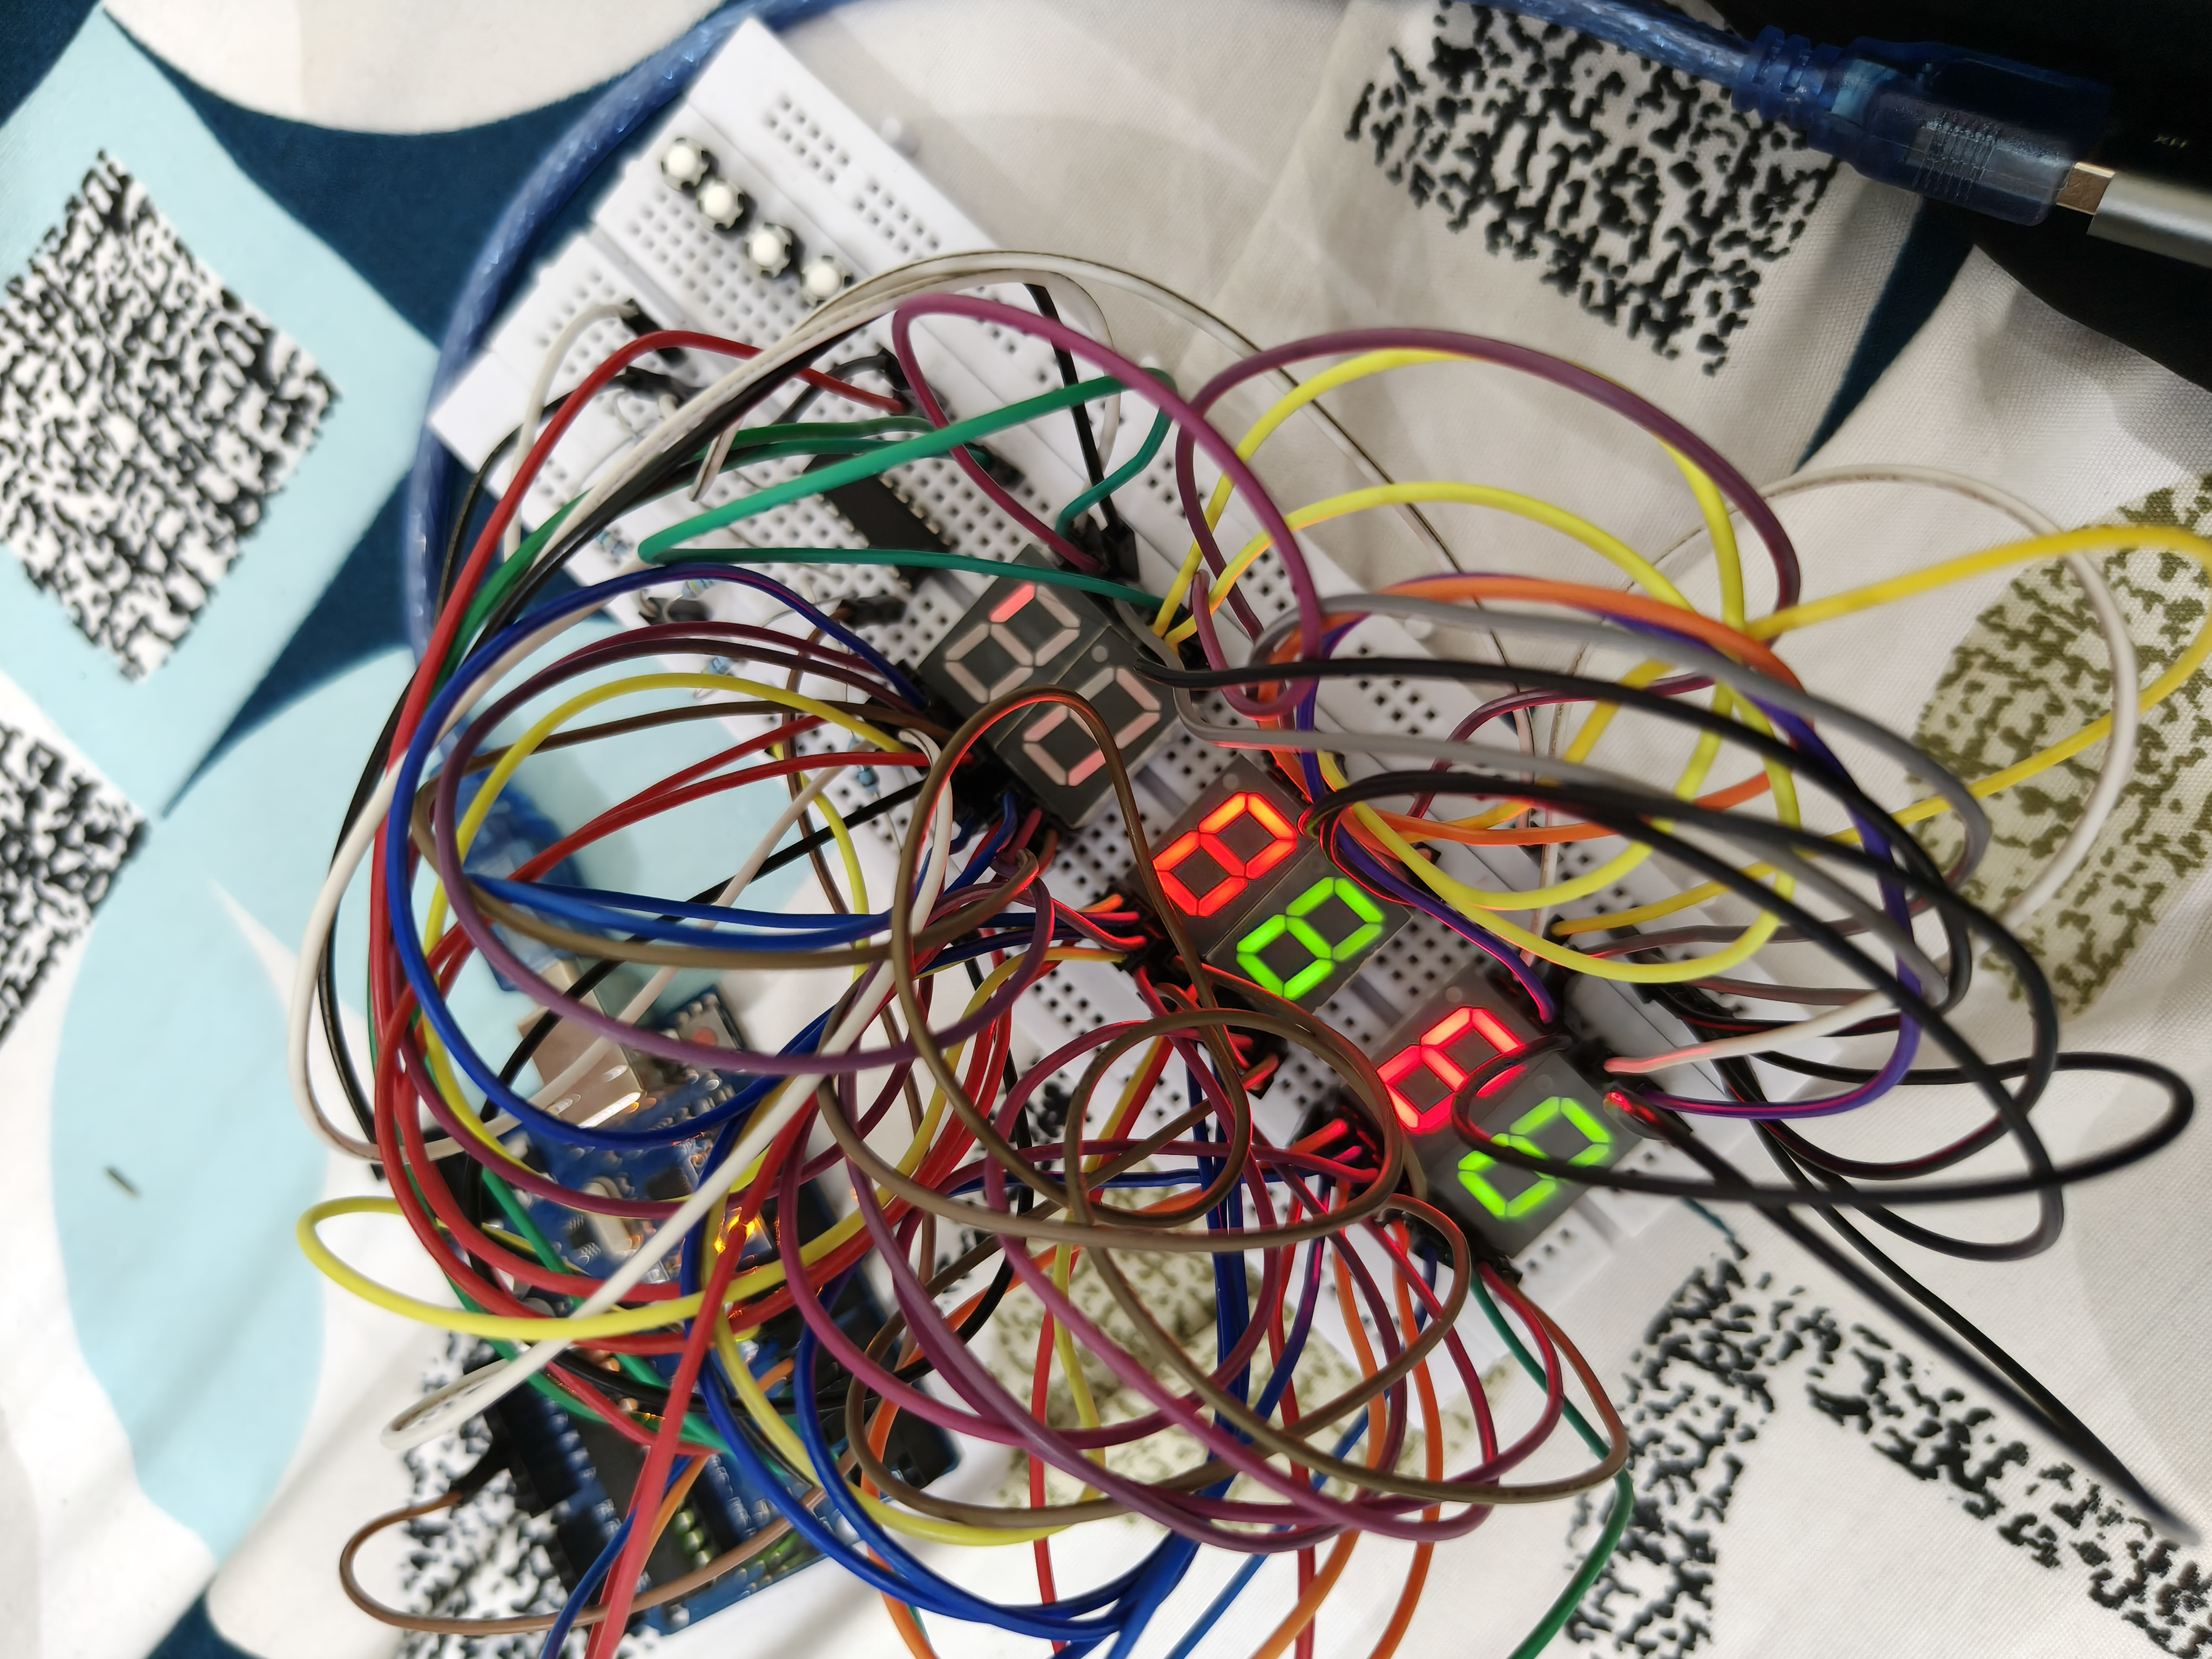
\includegraphics[width=0.88\textwidth,height=0.68\textheight,keepaspectratio]{images/1.jpg}
    \caption{Non-working single breadboard prototype due to malfunctioning displays.}
    \label{fig:visual-progress-1}
\end{figure}

\begin{figure}[H]
    \centering
    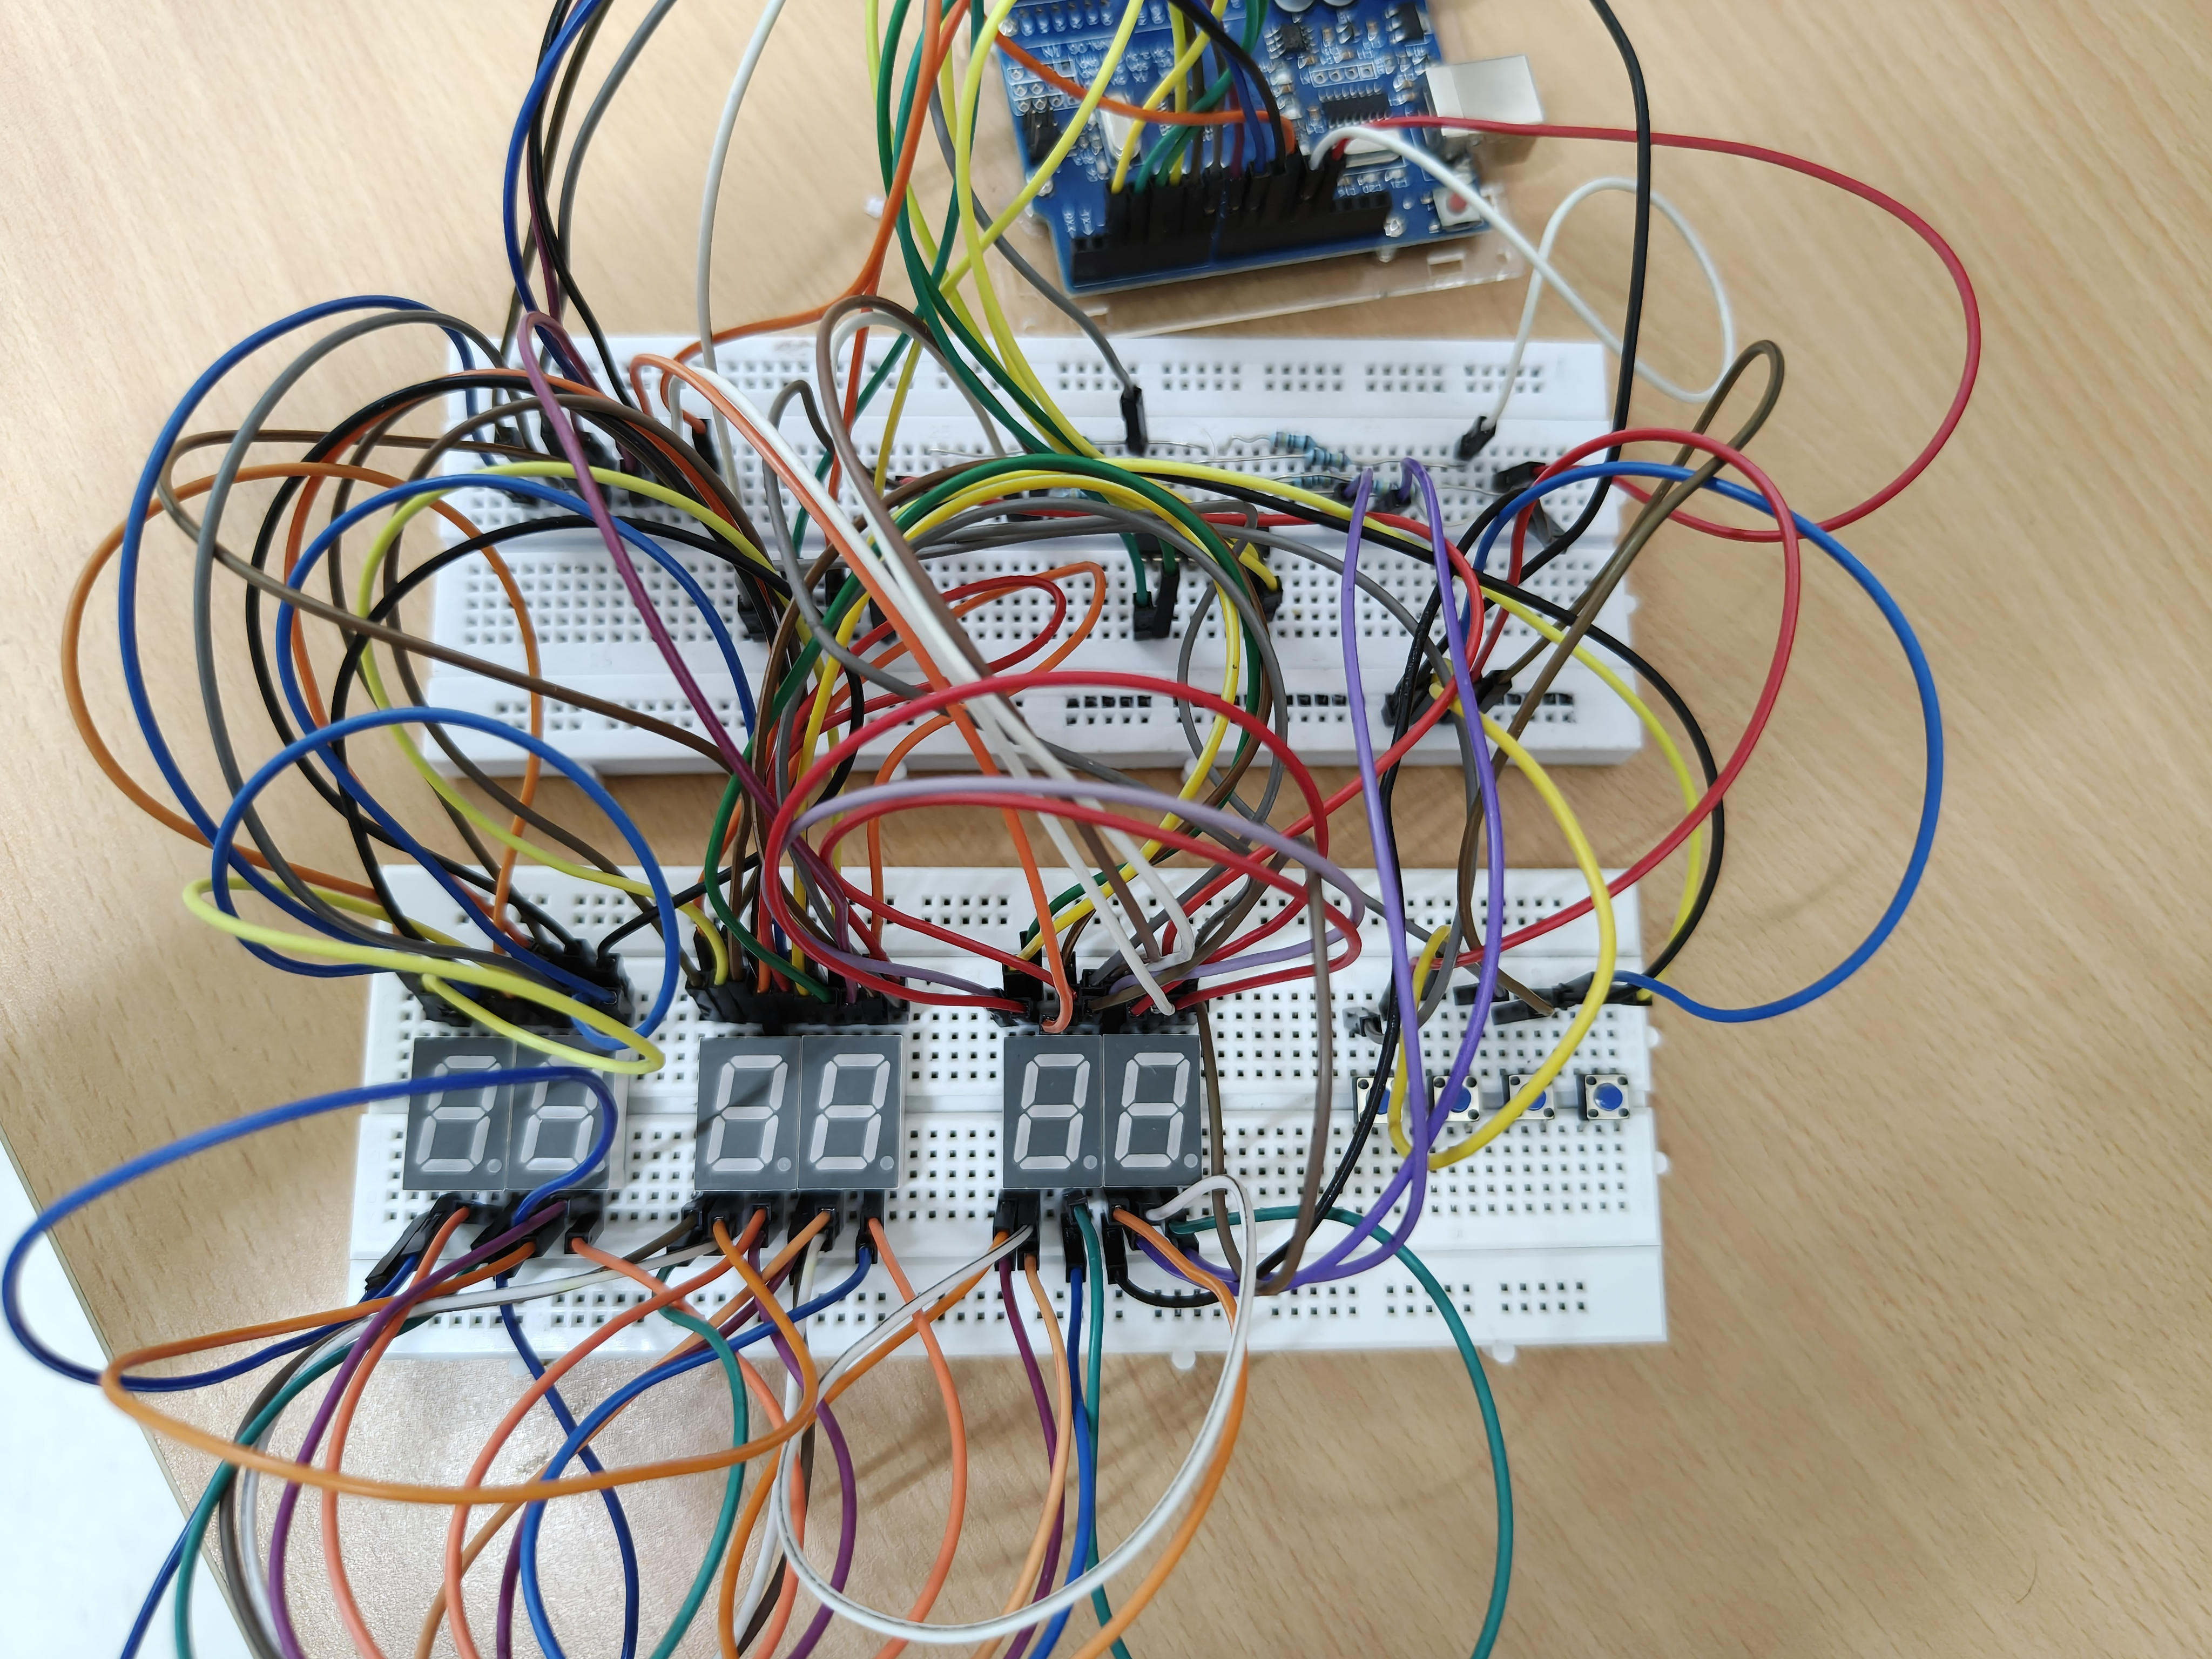
\includegraphics[width=0.88\textwidth,height=0.68\textheight,keepaspectratio]{images/2.jpg}
    \caption{Working Prototype 1 with two breadboards.}
    \label{fig:visual-progress-2}
\end{figure}

\begin{figure}[H]
    \centering
    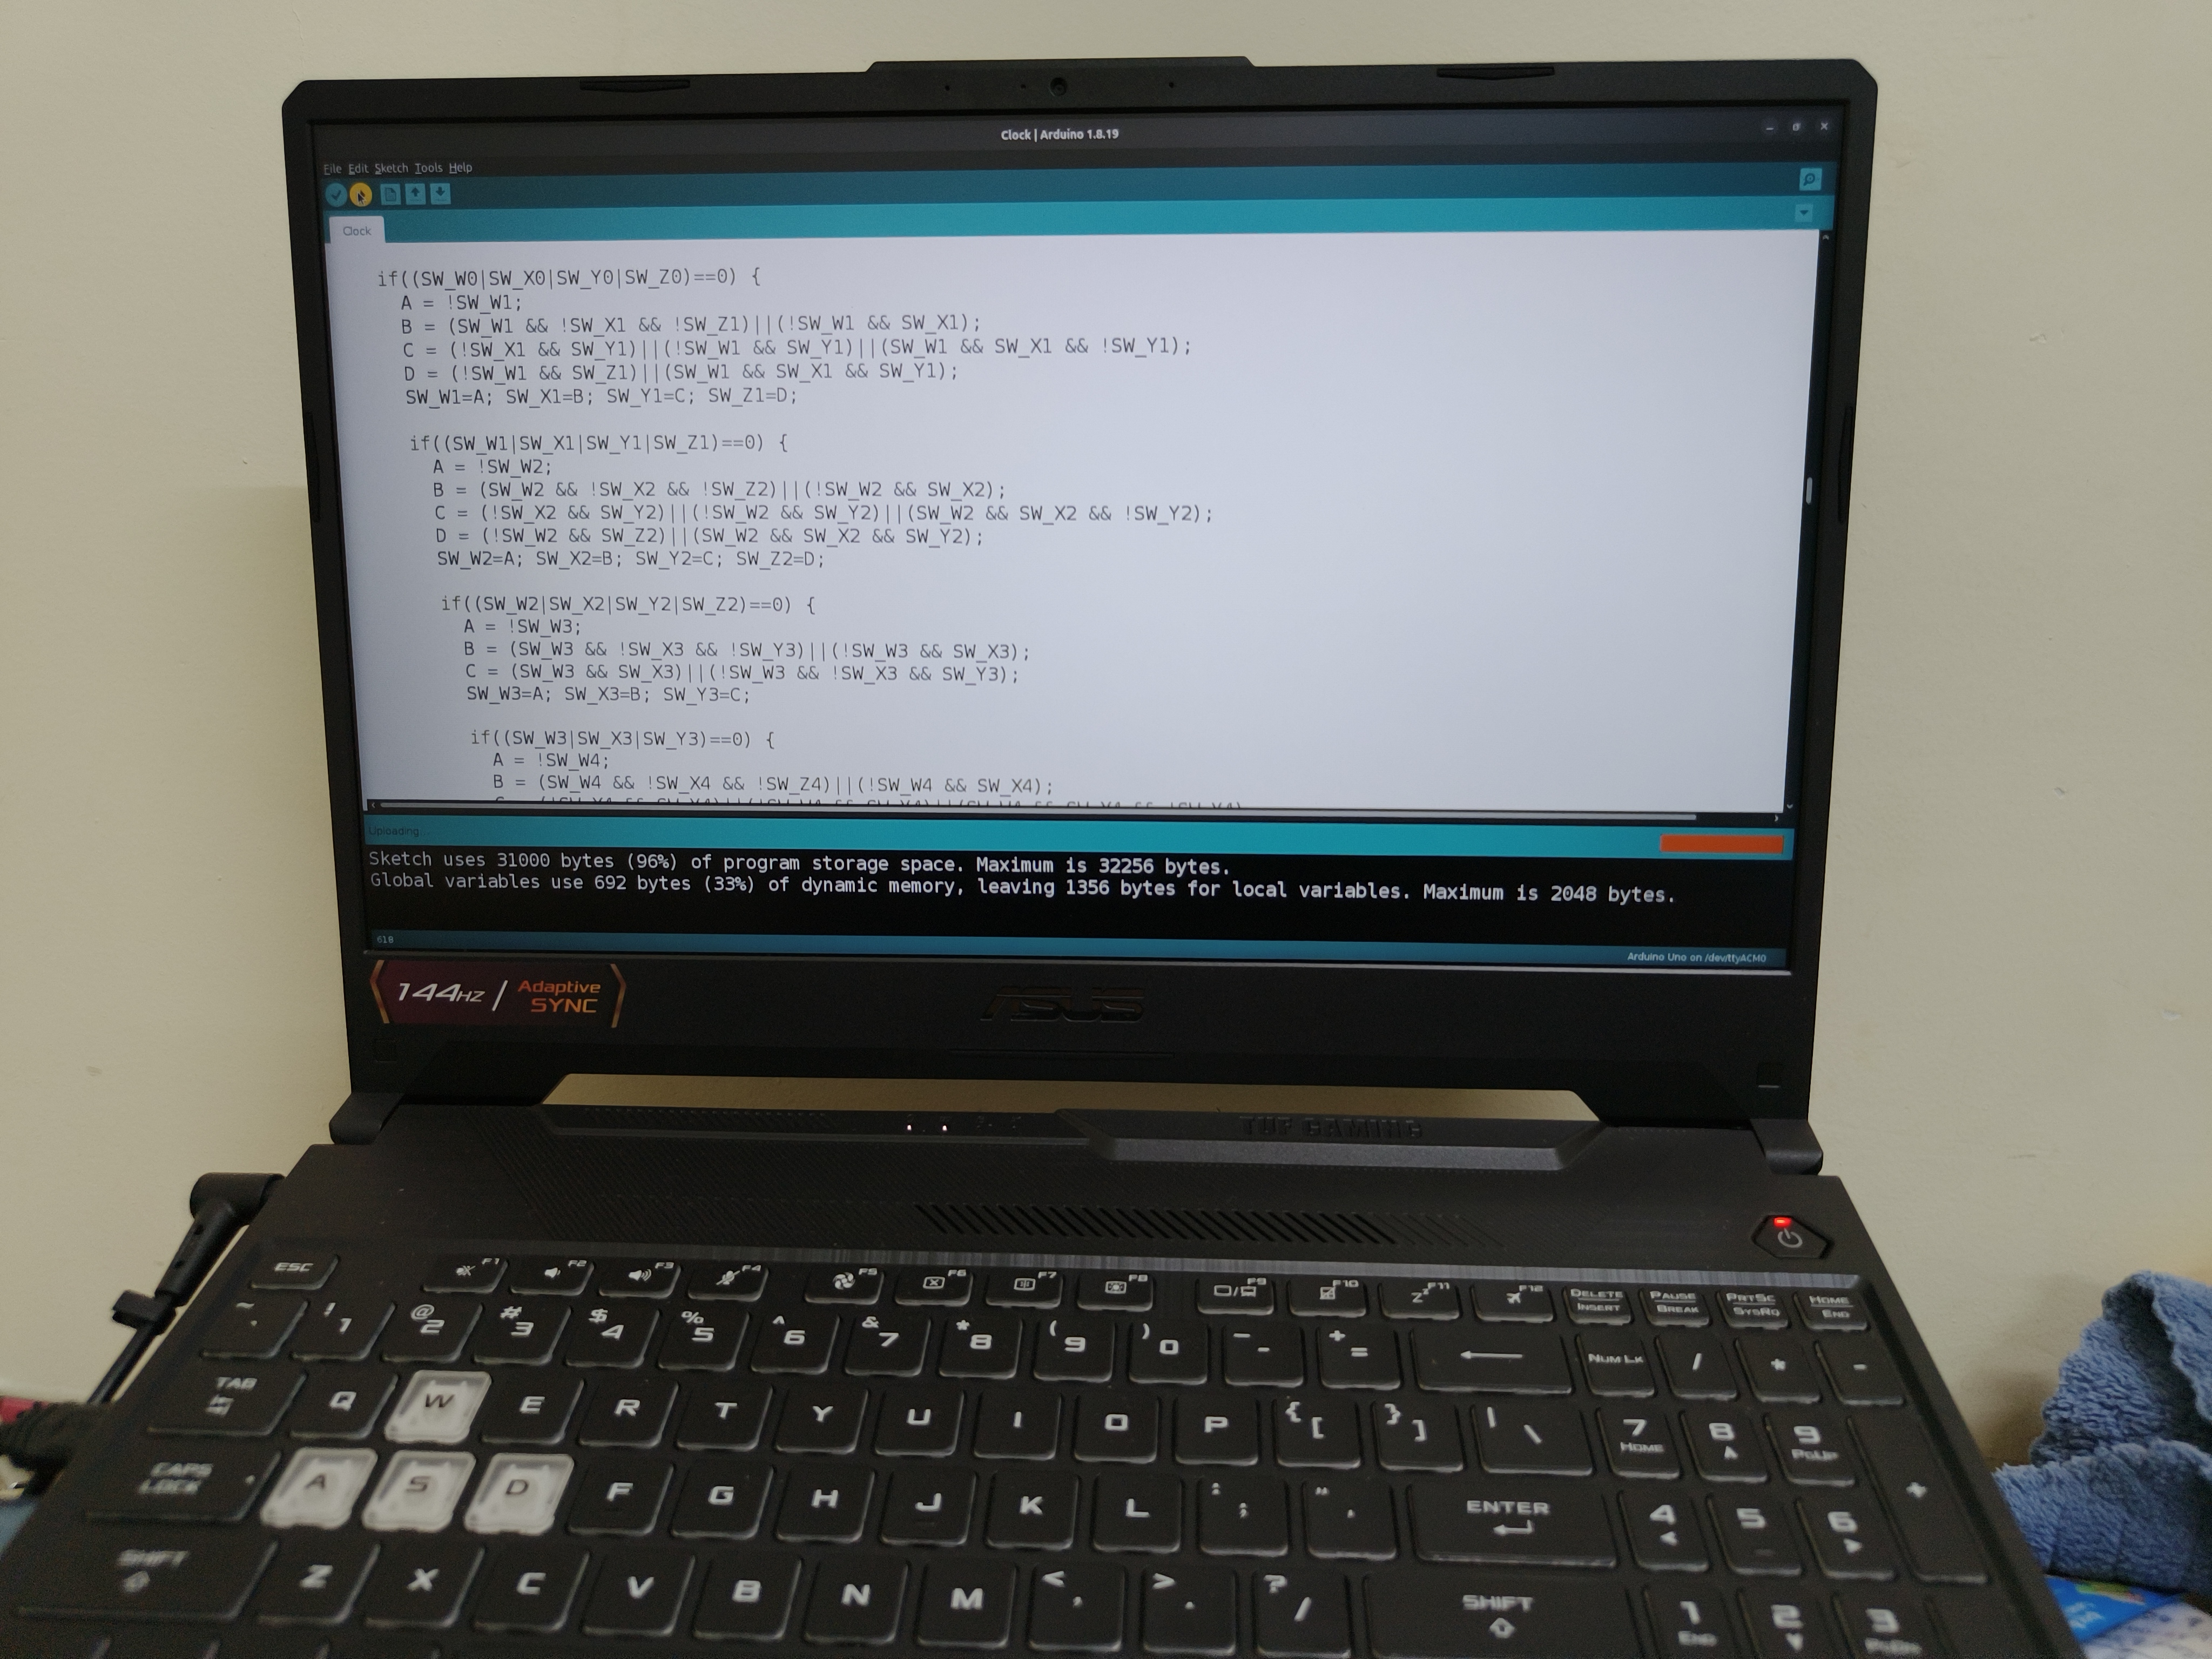
\includegraphics[width=0.88\textwidth,height=0.68\textheight,keepaspectratio]{images/3.jpg}
    \caption{Code uploading to the Arduino.}
    \label{fig:visual-progress-3}
\end{figure}

\begin{figure}[H]
    \centering
    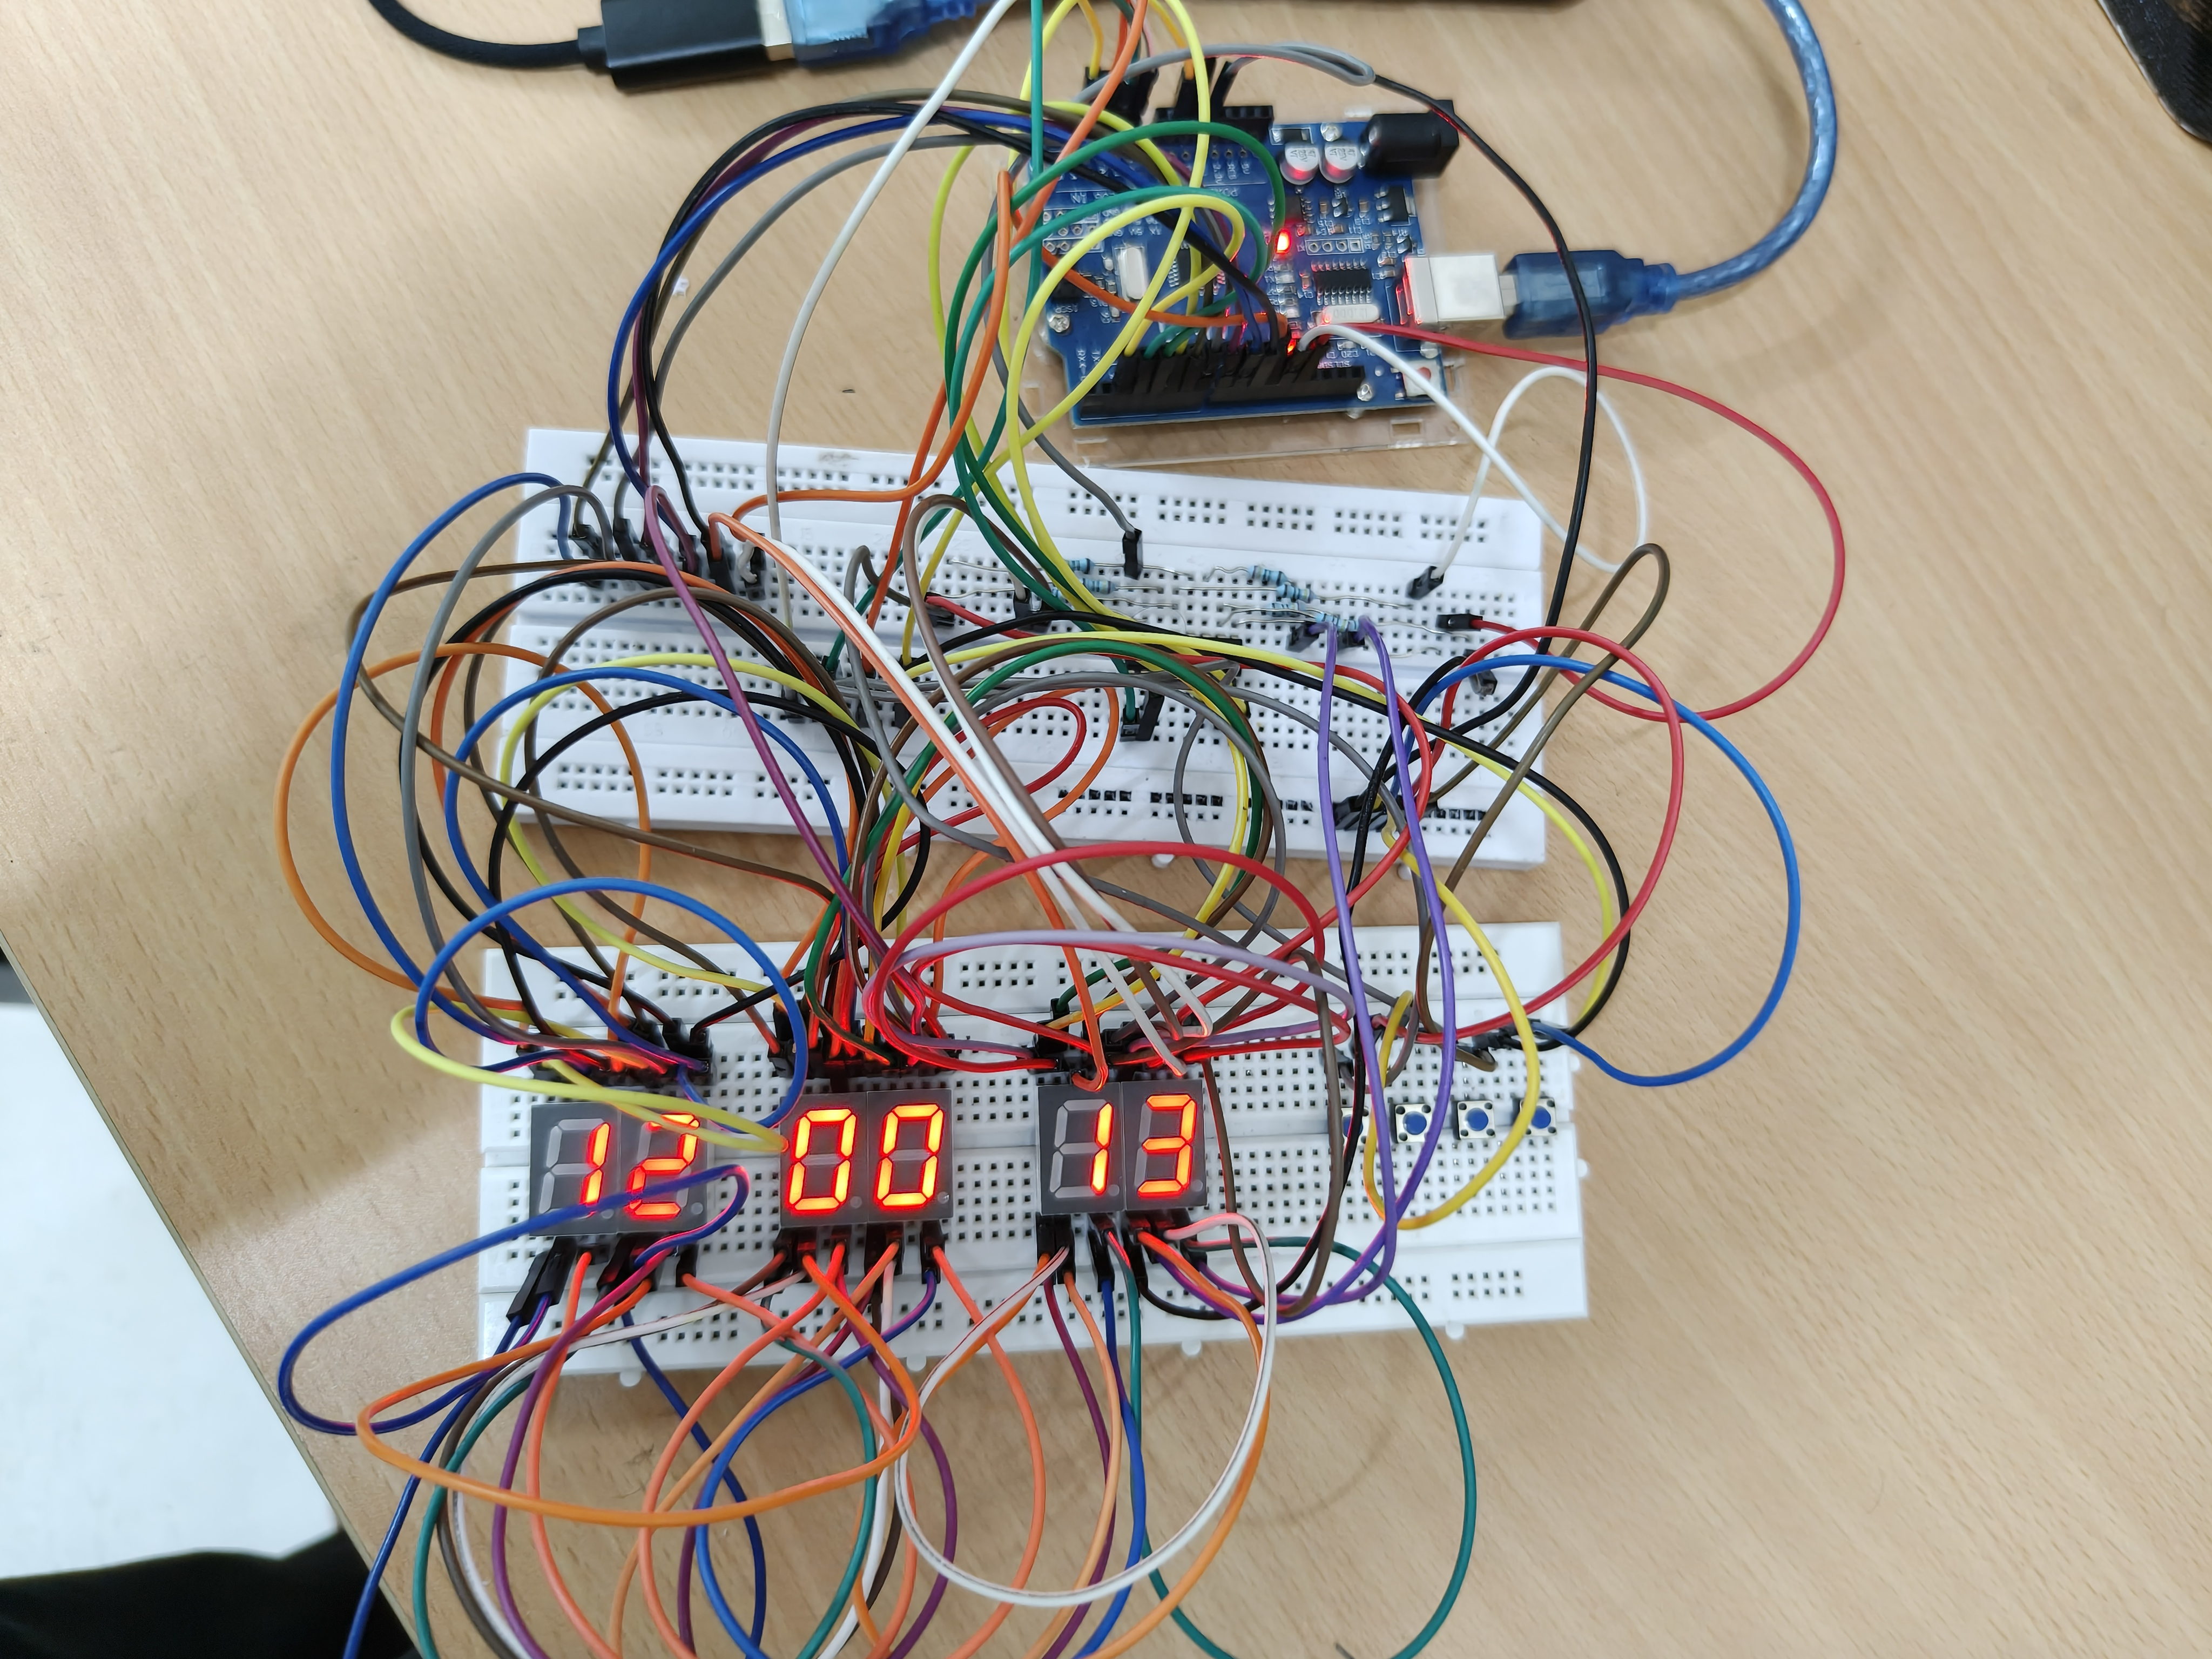
\includegraphics[width=0.88\textwidth,height=0.68\textheight,keepaspectratio]{images/4.jpg}
    \caption{Working Prototype 1 powered on.}
    \label{fig:visual-progress-4}
\end{figure}

\begin{figure}[H]
    \centering
    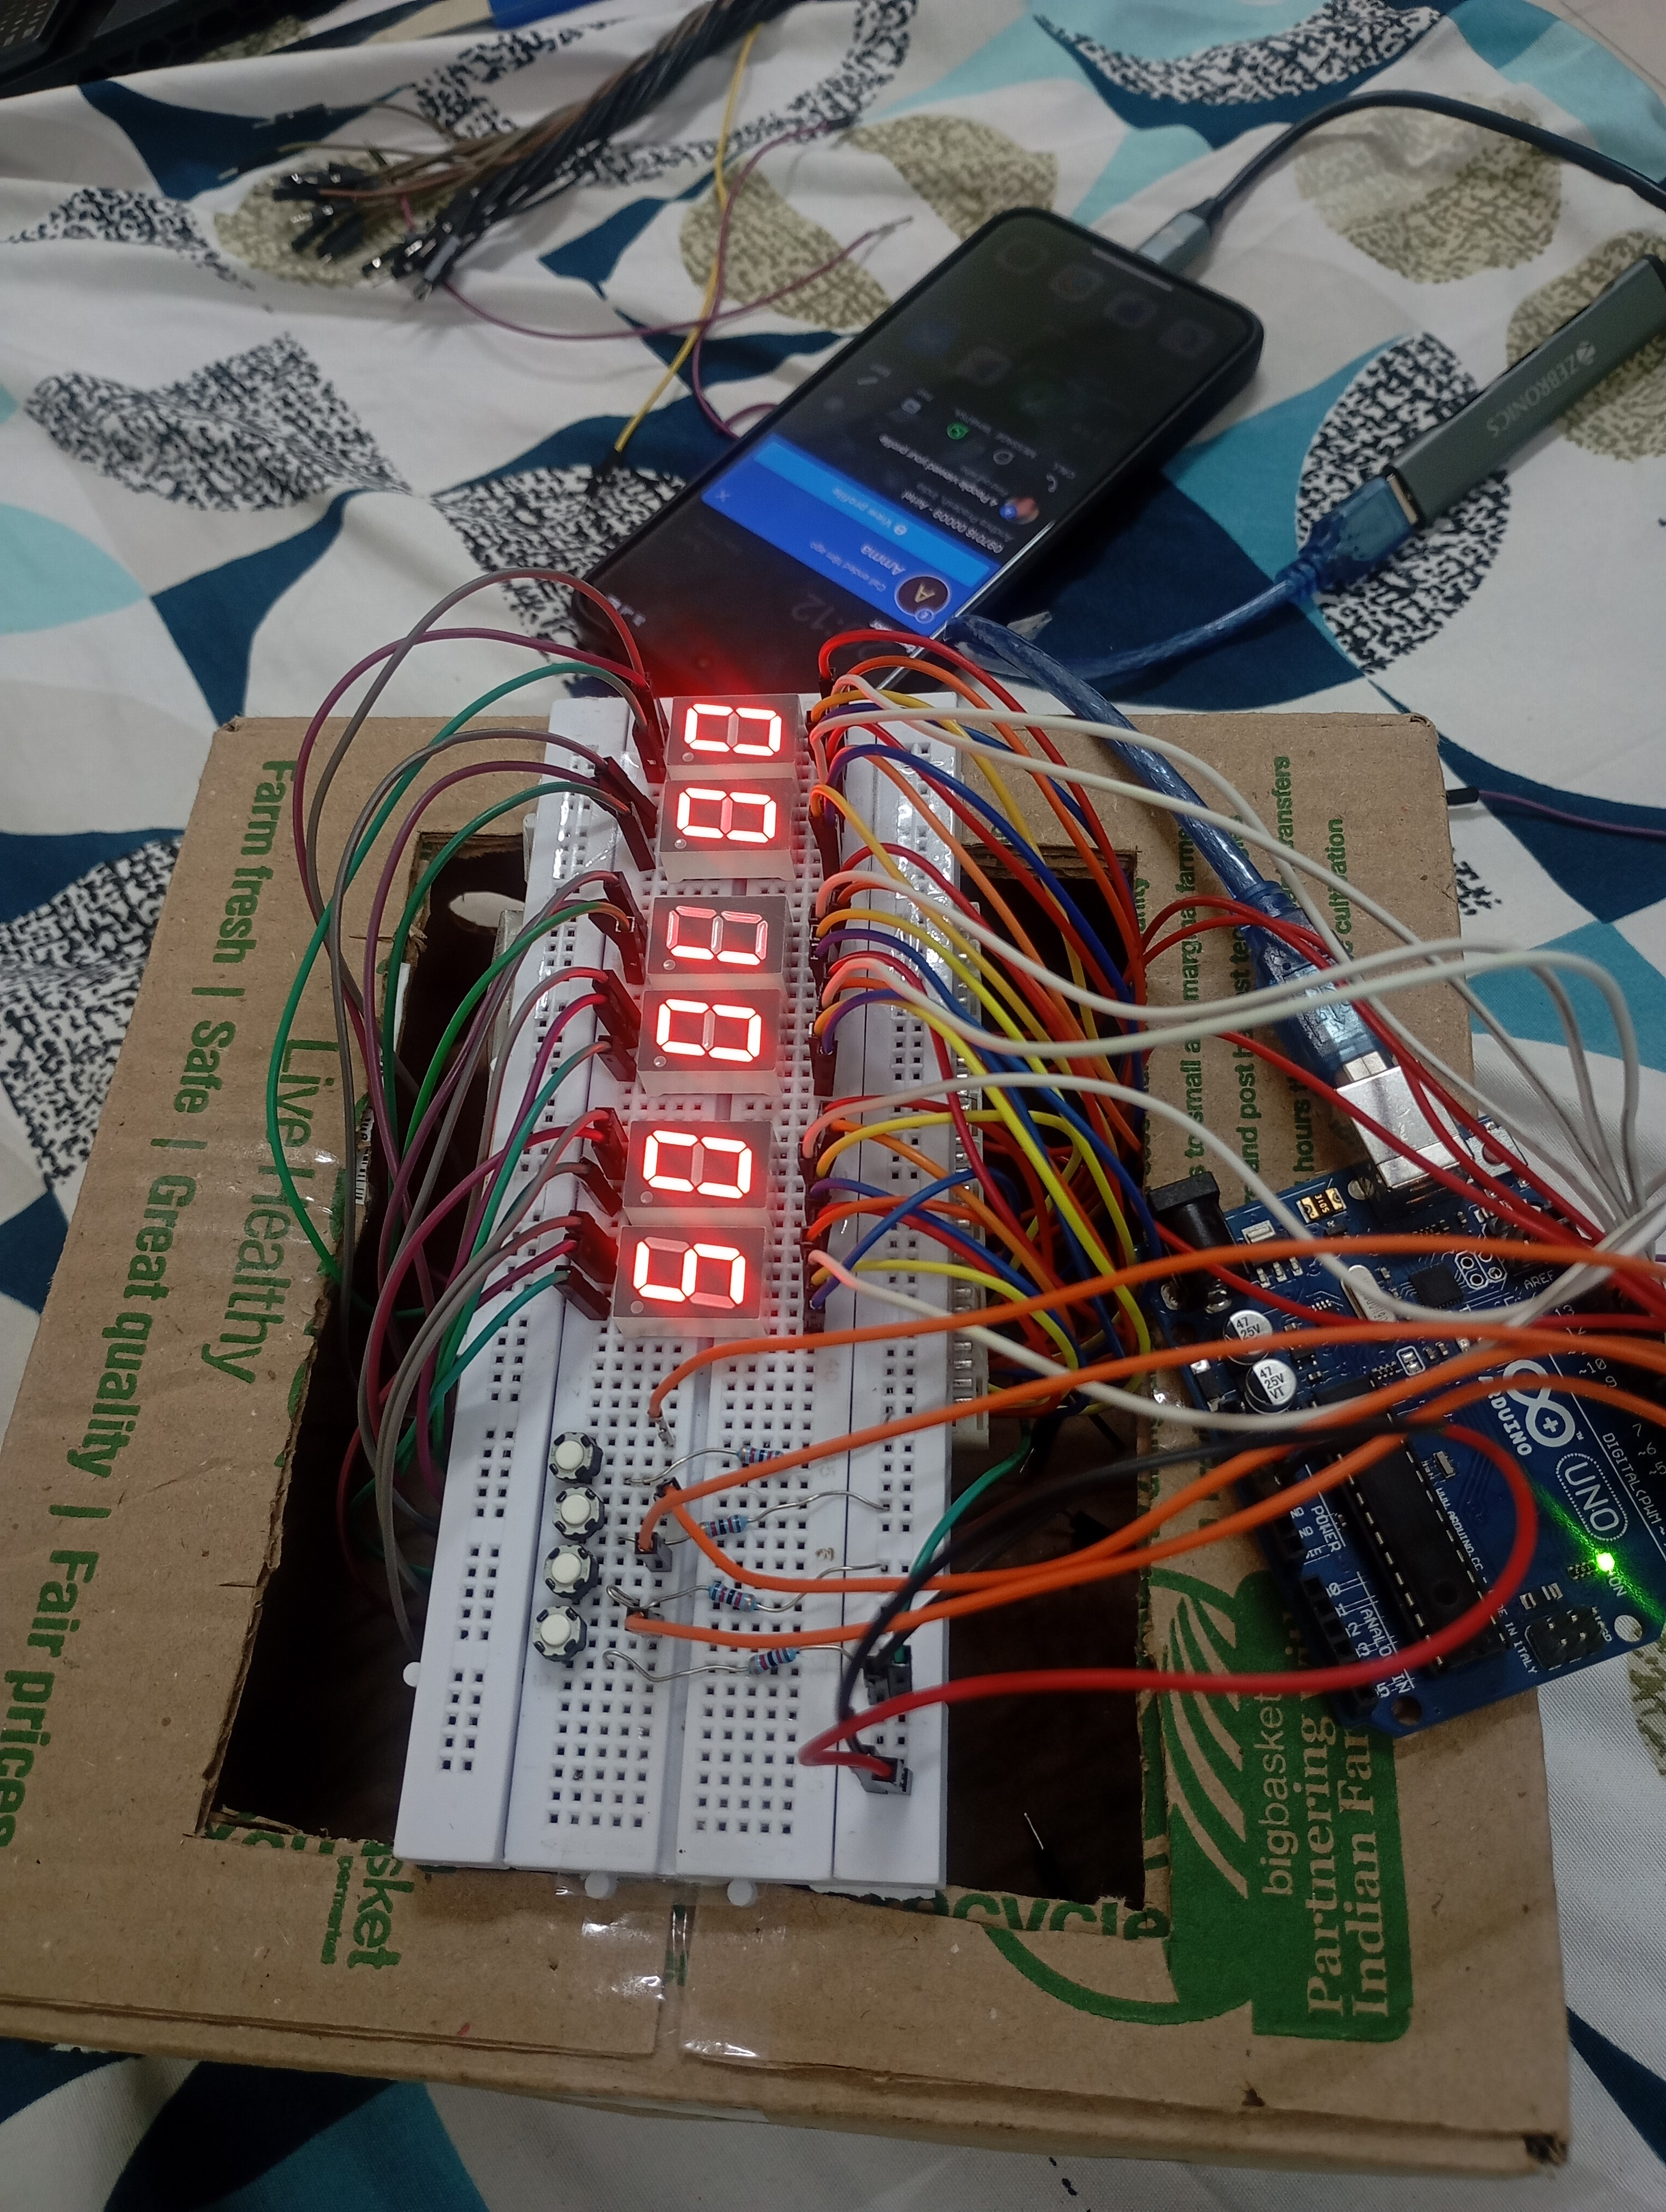
\includegraphics[width=0.88\textwidth,height=0.68\textheight,keepaspectratio]{images/5.jpg}
    \caption{Boxing thought and enclosure planning stage.}
    \label{fig:visual-progress-5}
\end{figure}

\begin{figure}[H]
    \centering
    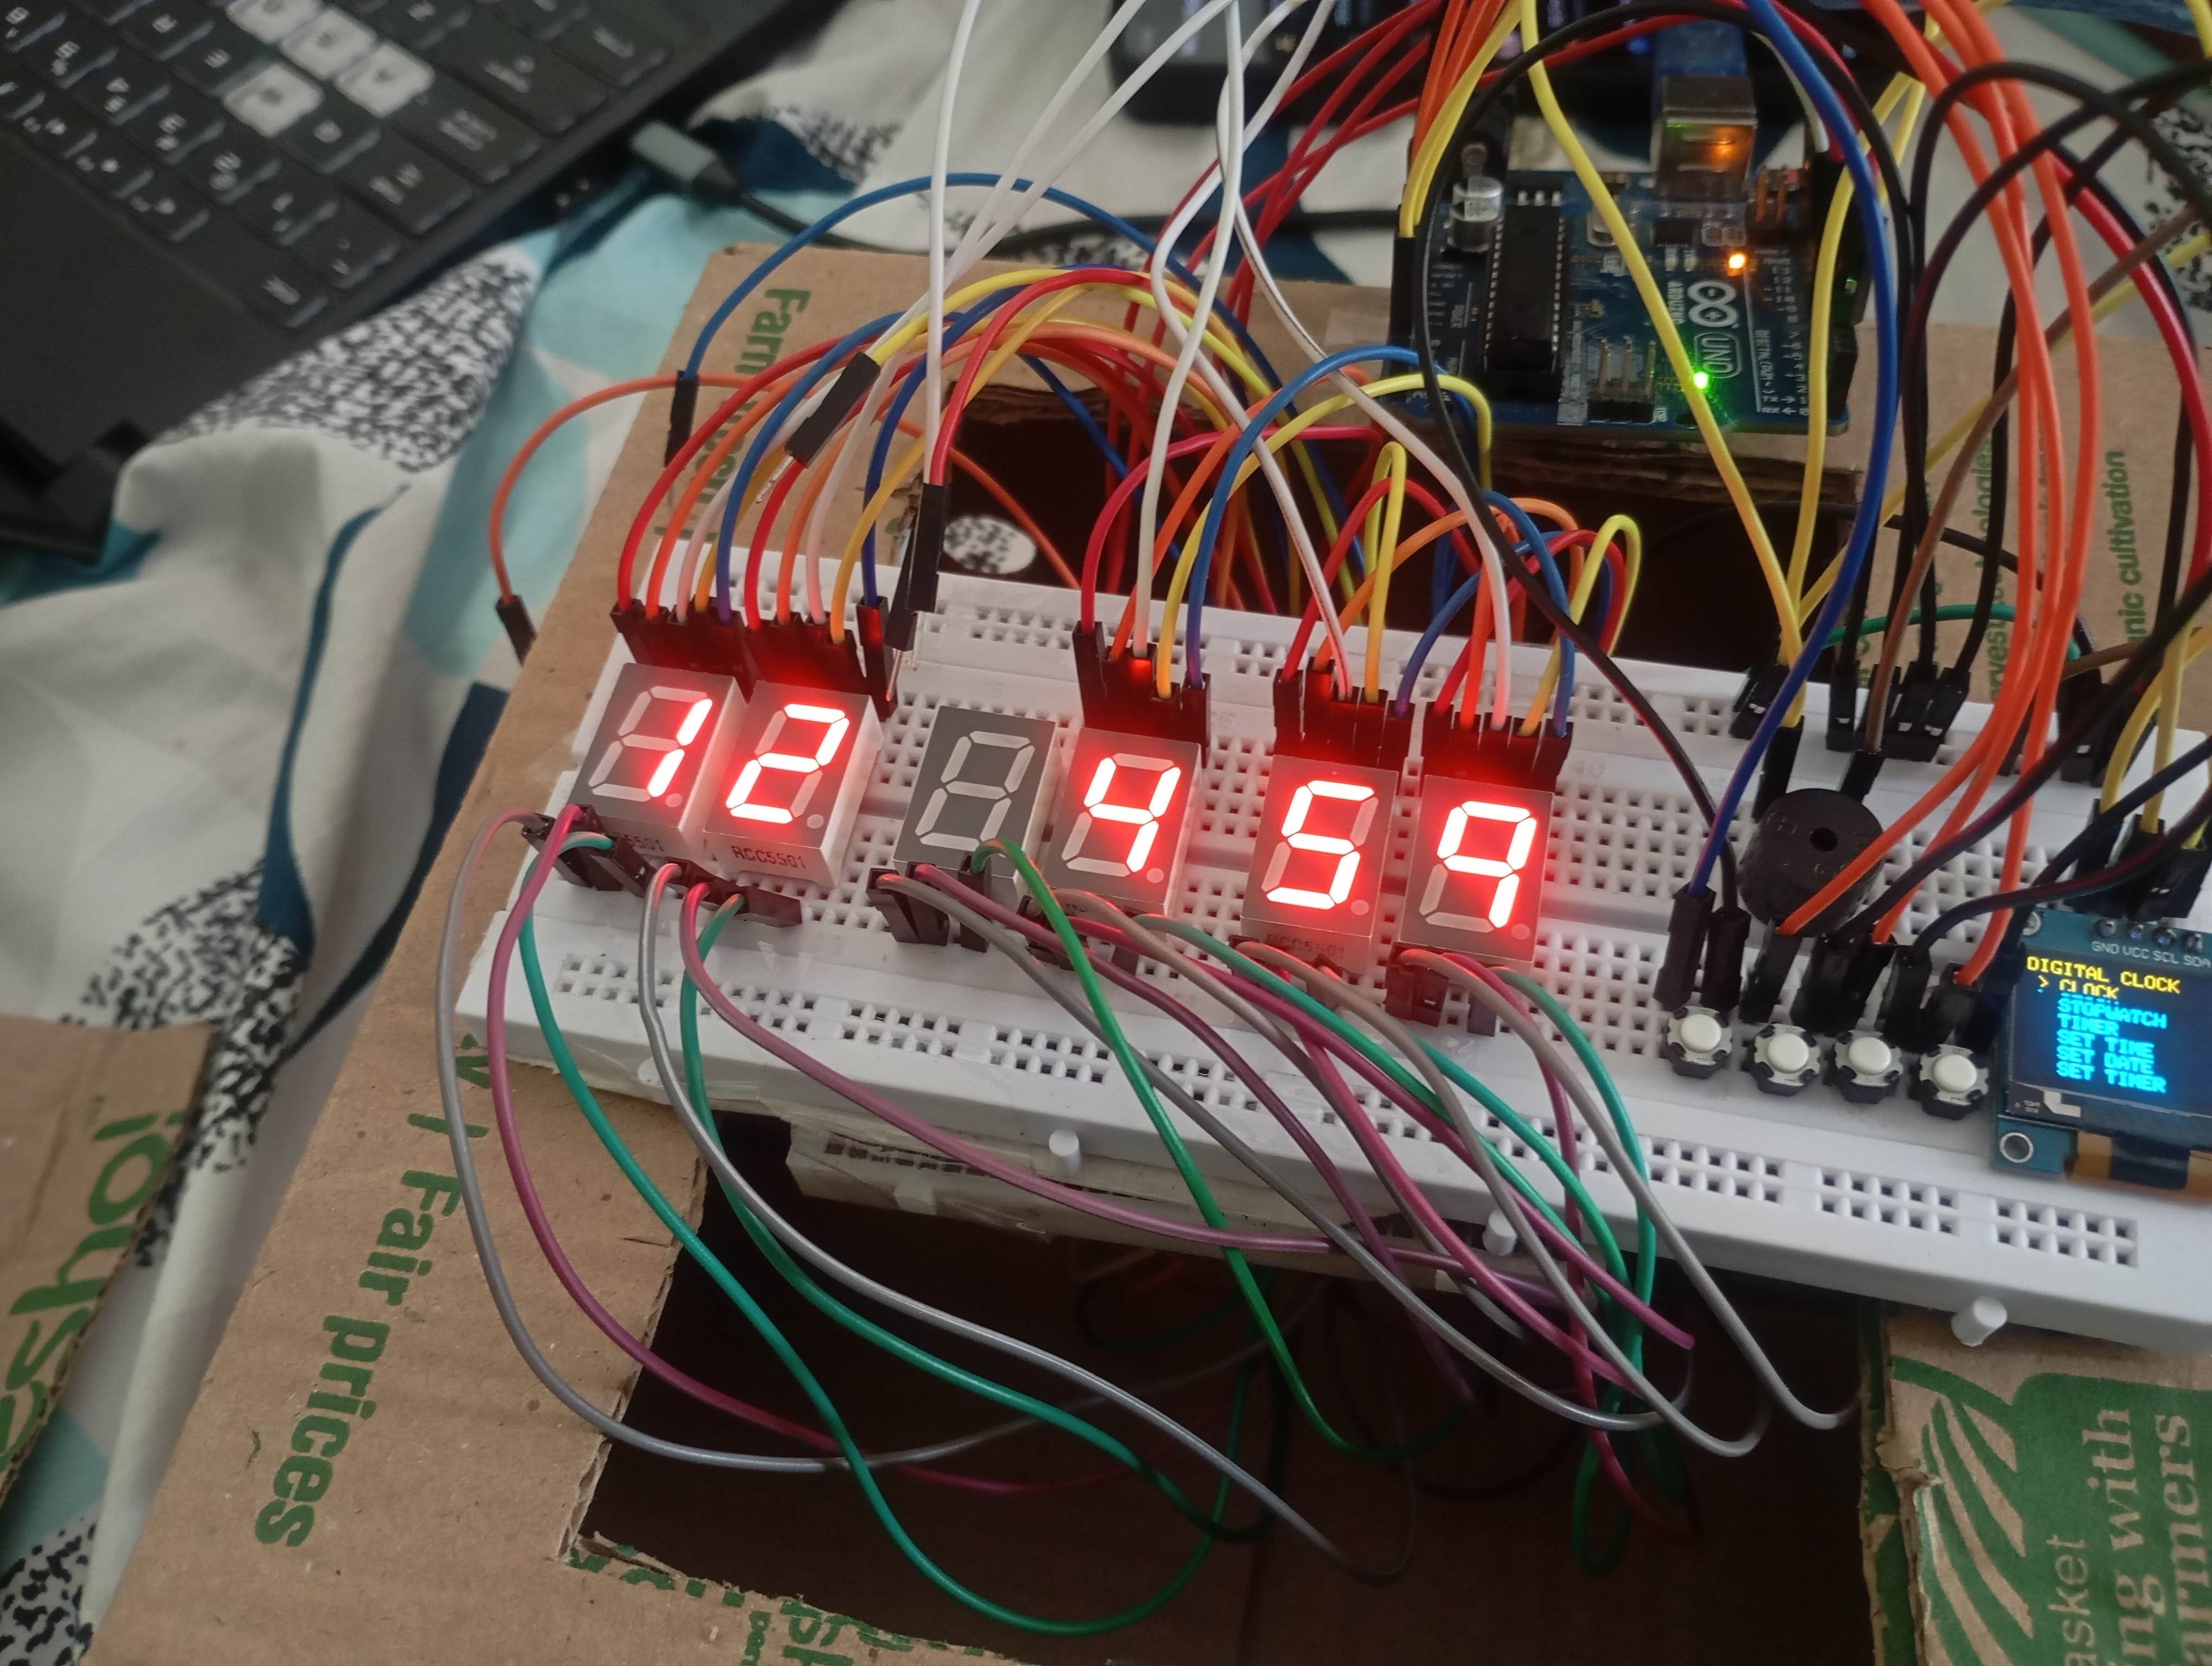
\includegraphics[width=0.88\textwidth,height=0.68\textheight,keepaspectratio]{images/6.jpg}
    \caption{Addition of the OLED secondary display.}
    \label{fig:visual-progress-6}
\end{figure}

\begin{figure}[H]
    \centering
    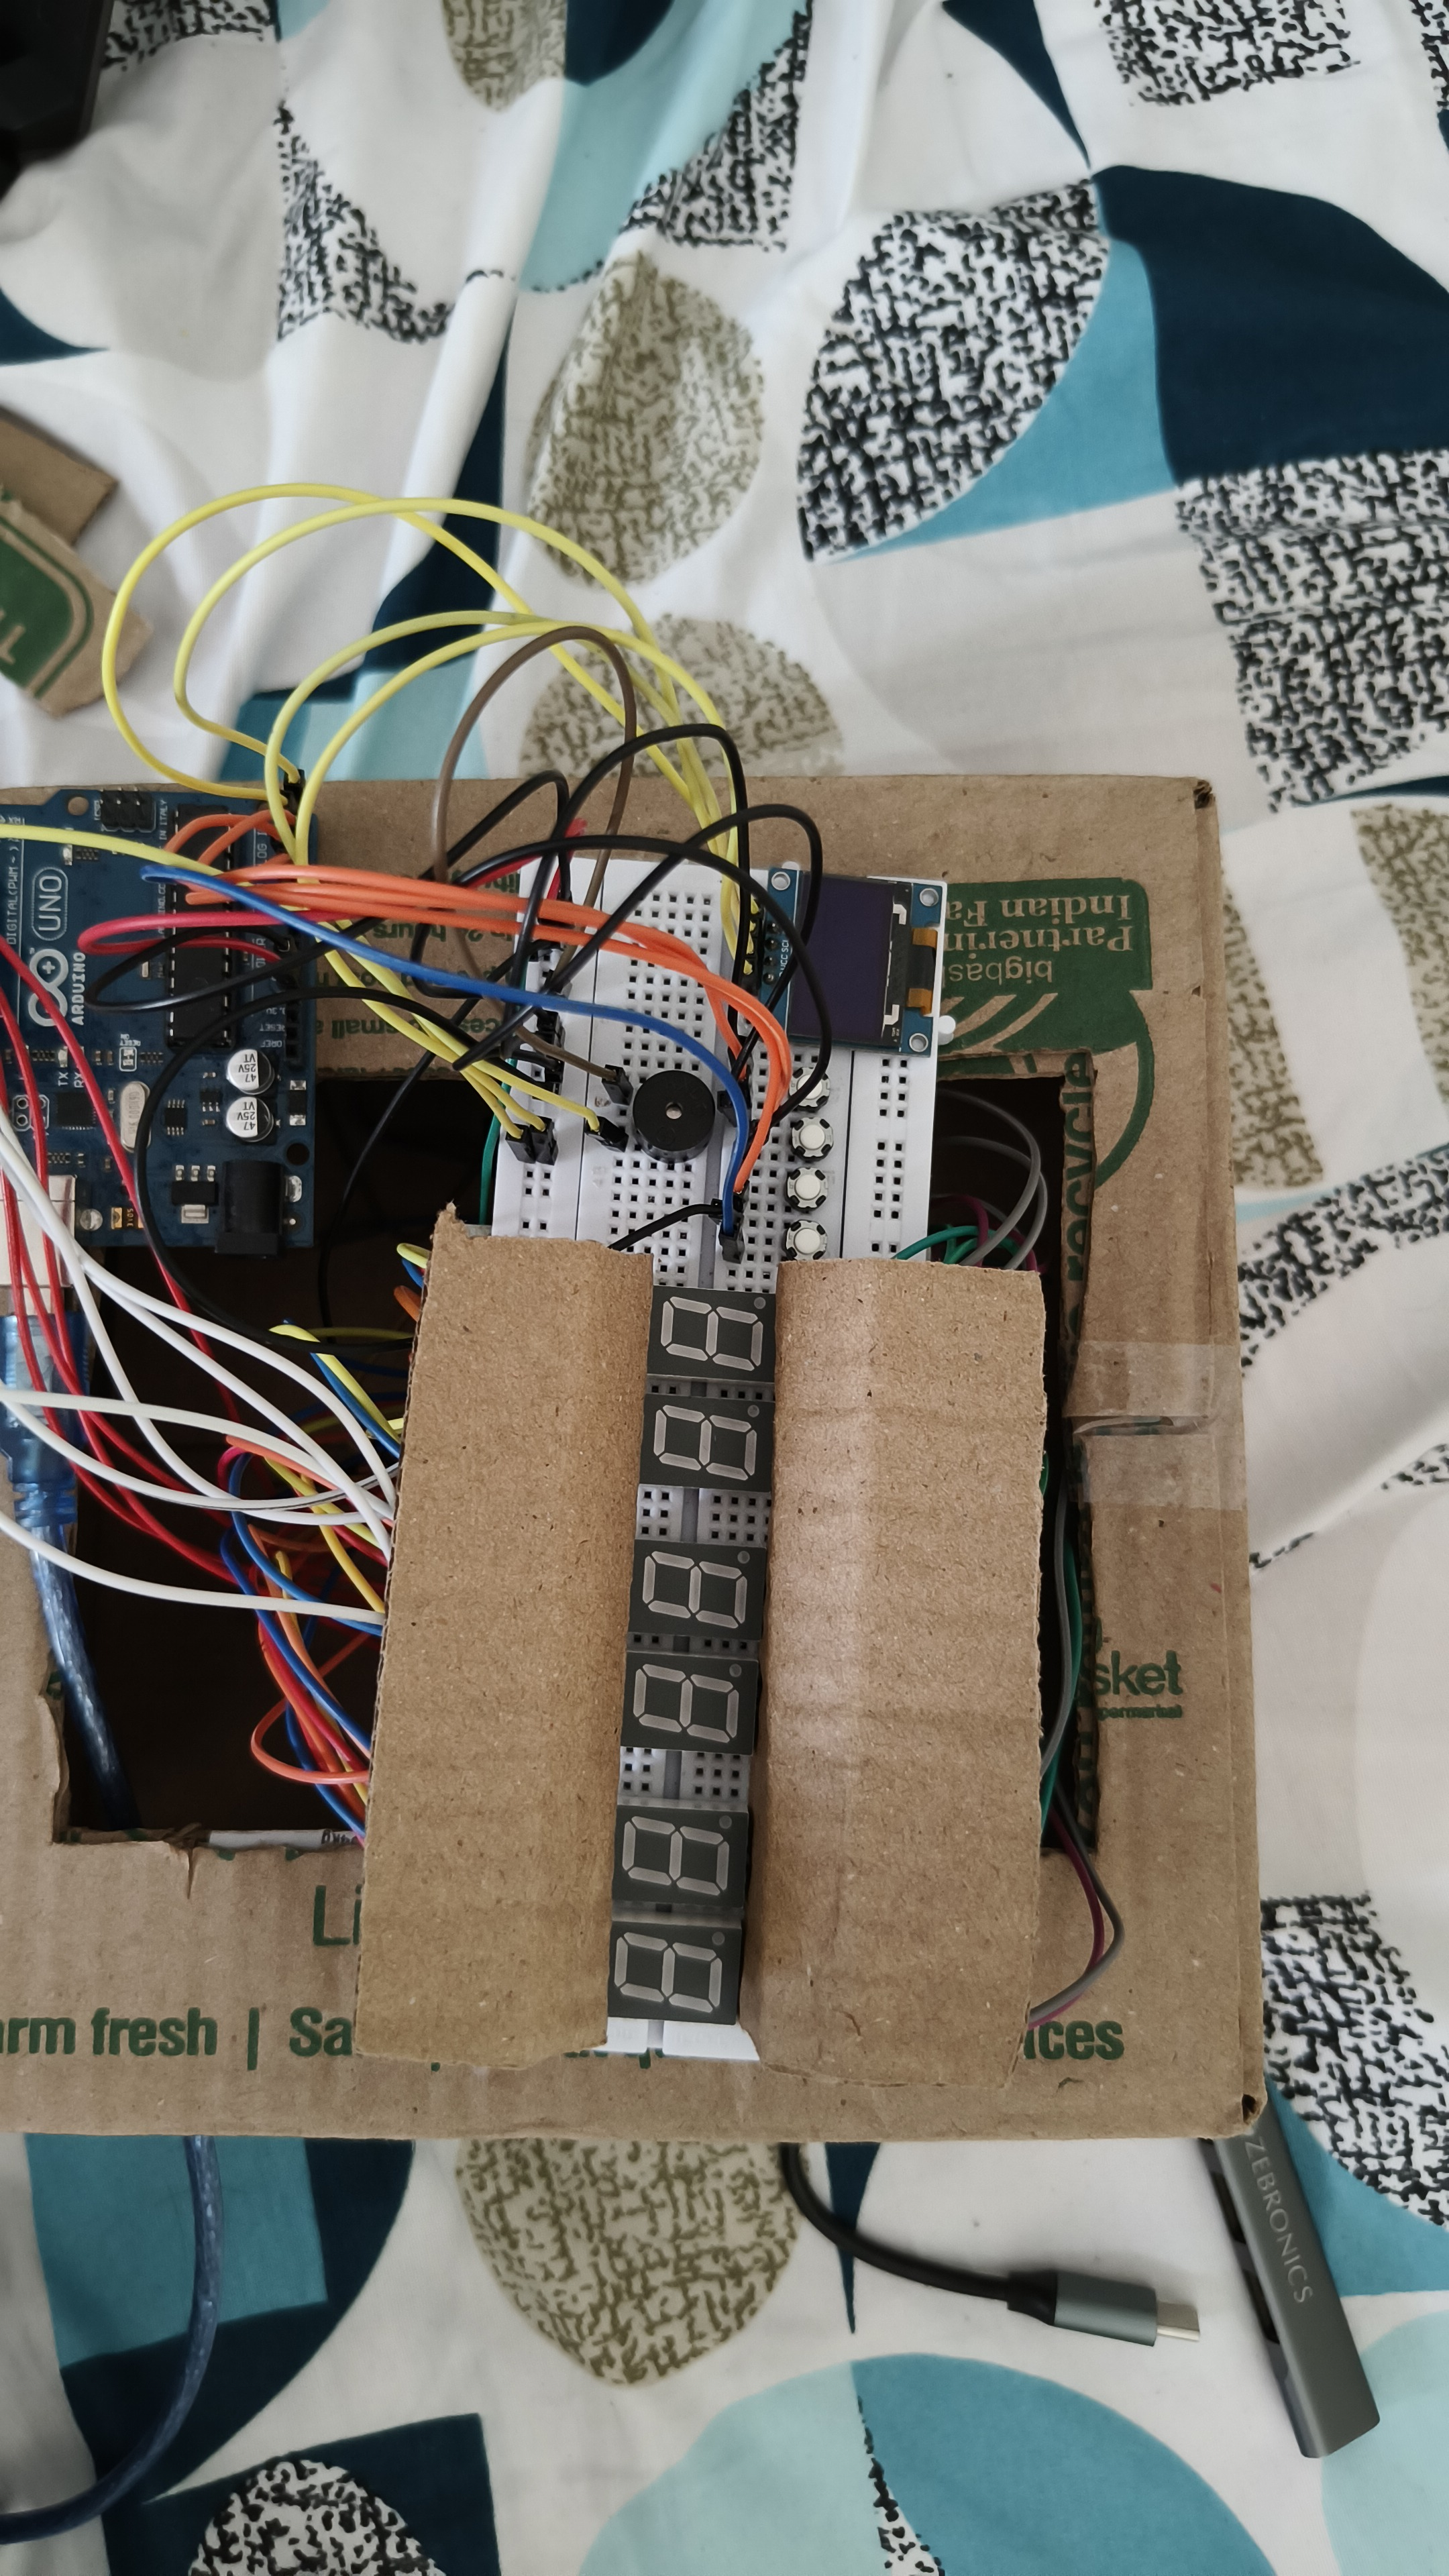
\includegraphics[width=0.88\textwidth,height=0.68\textheight,keepaspectratio]{images/7.jpg}
    \caption{Cardboard insulation of the digits along with the buzzer.}
    \label{fig:visual-progress-7}
\end{figure}

\begin{figure}[H]
    \centering
    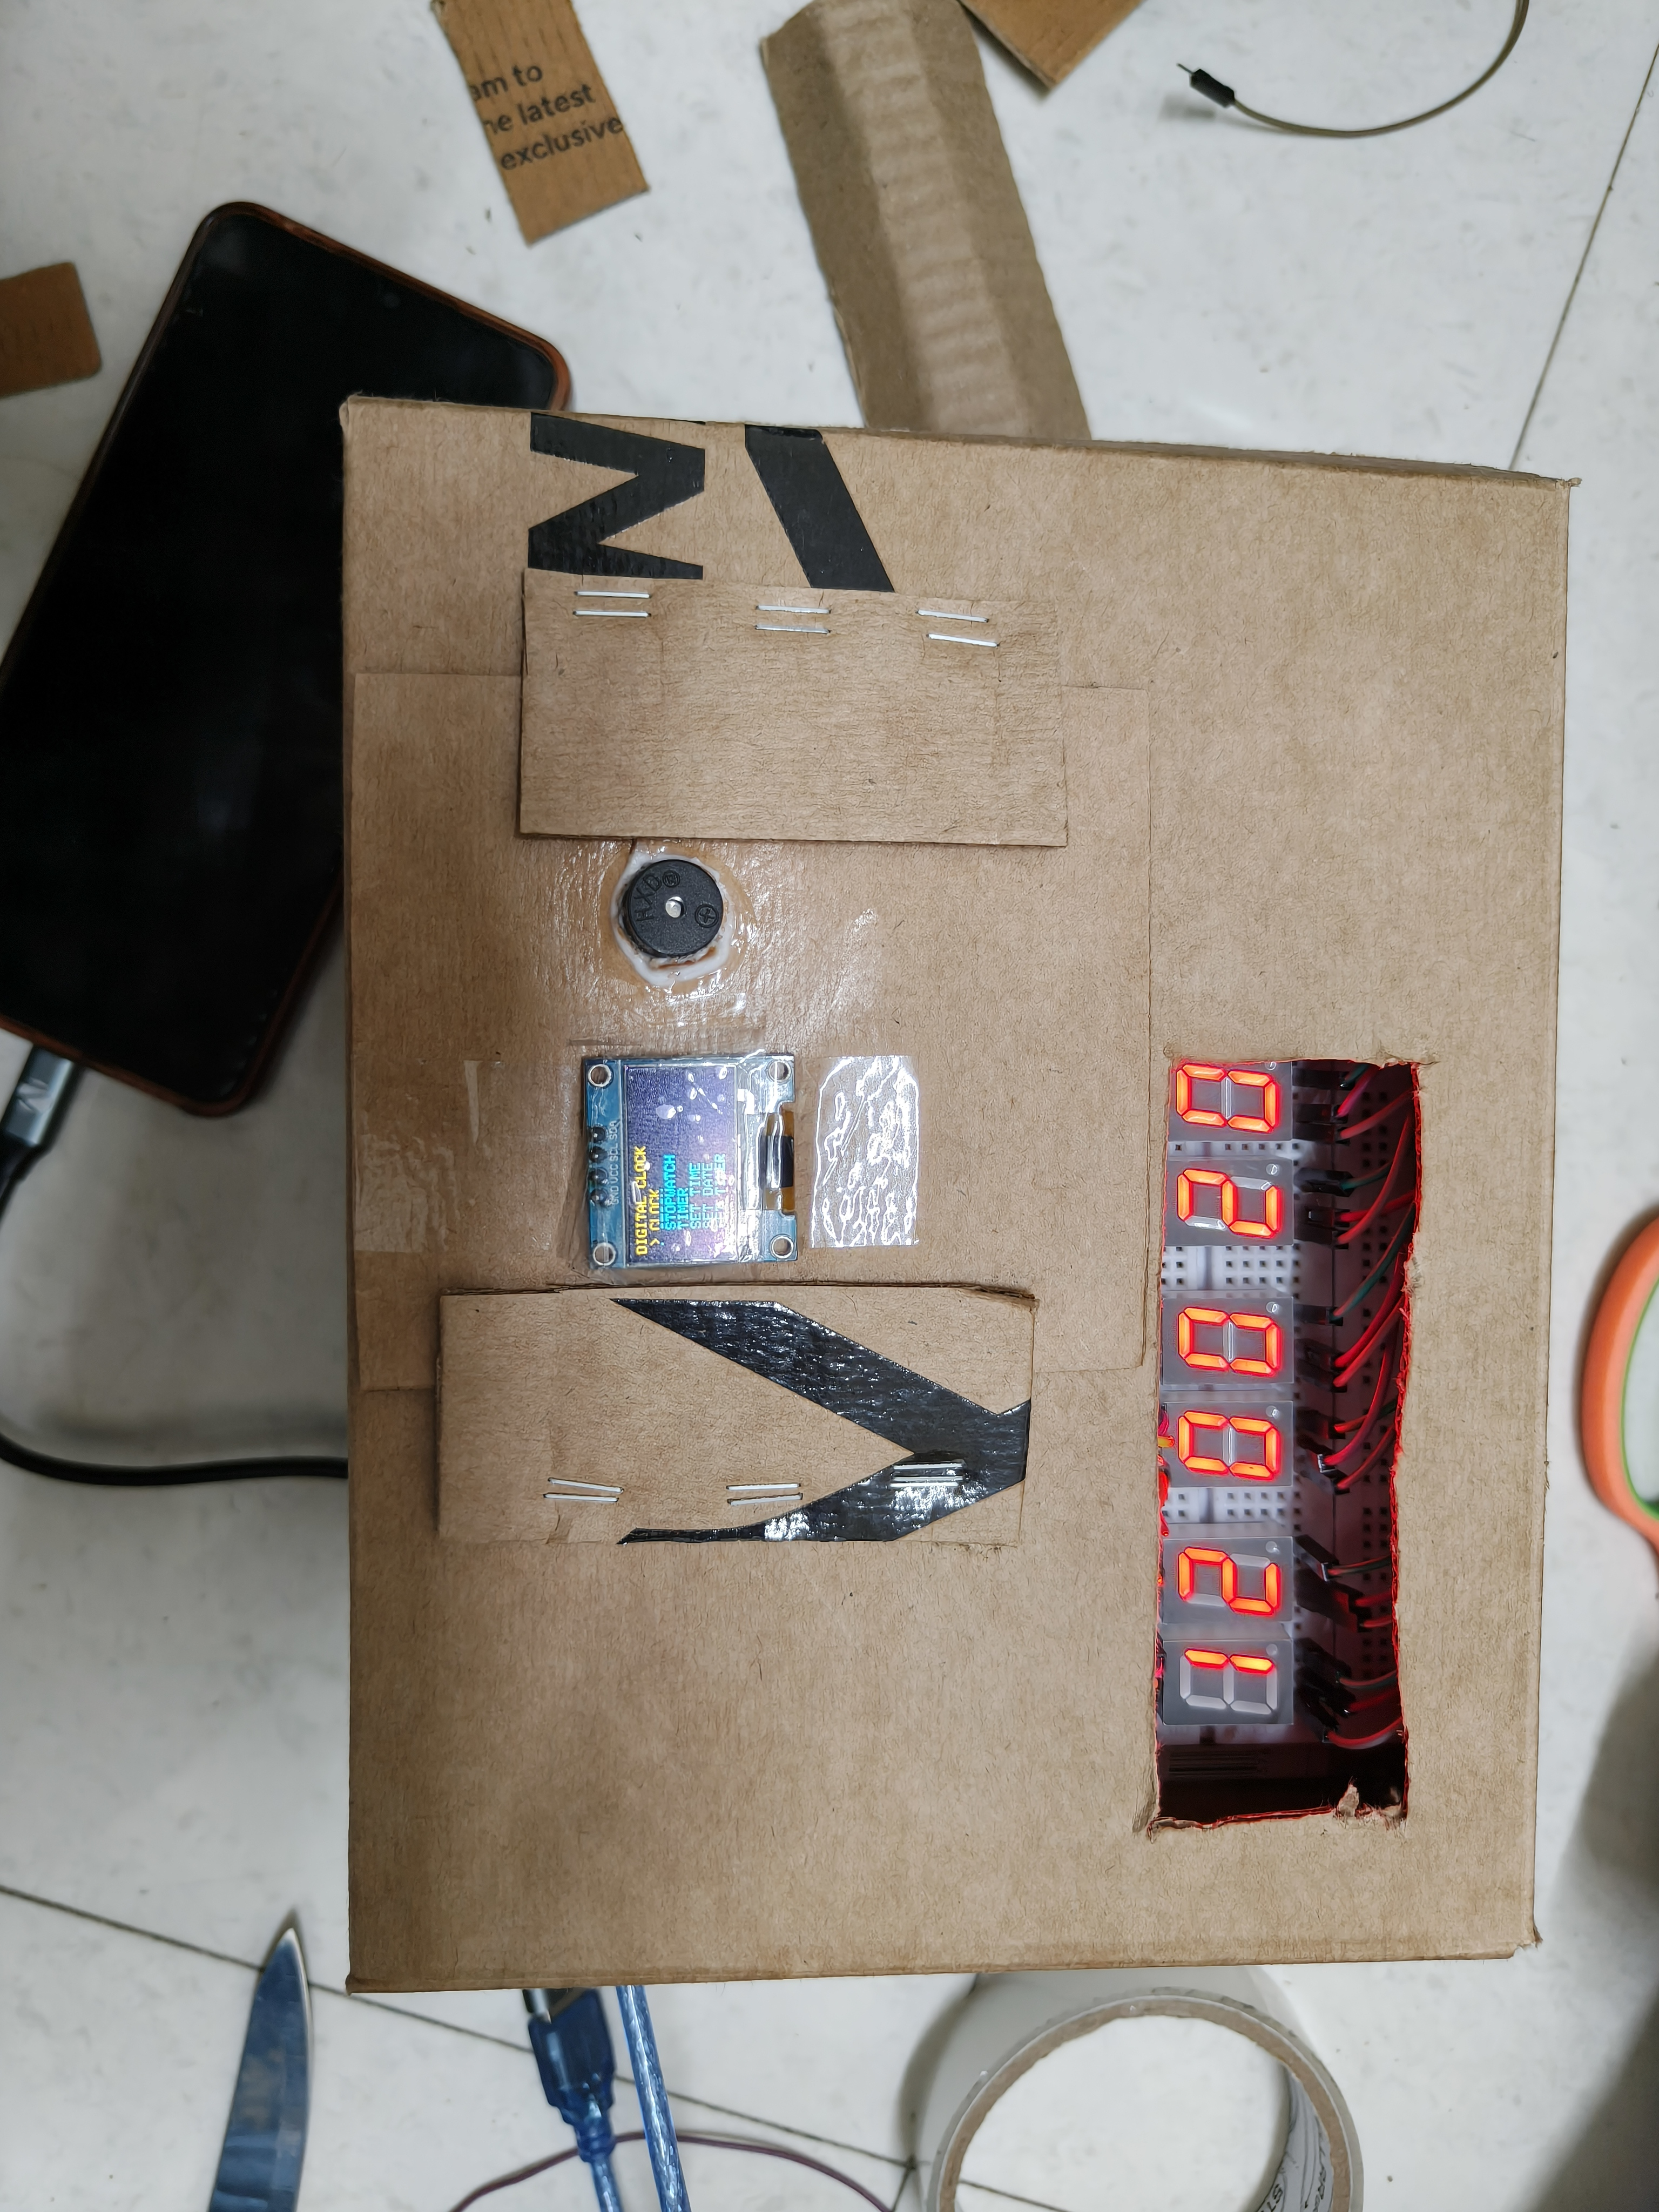
\includegraphics[width=0.88\textwidth,height=0.68\textheight,keepaspectratio]{images/8.jpg}
    \caption{No-touch-sensor model.}
    \label{fig:visual-progress-8}
\end{figure}

\begin{figure}[H]
    \centering
    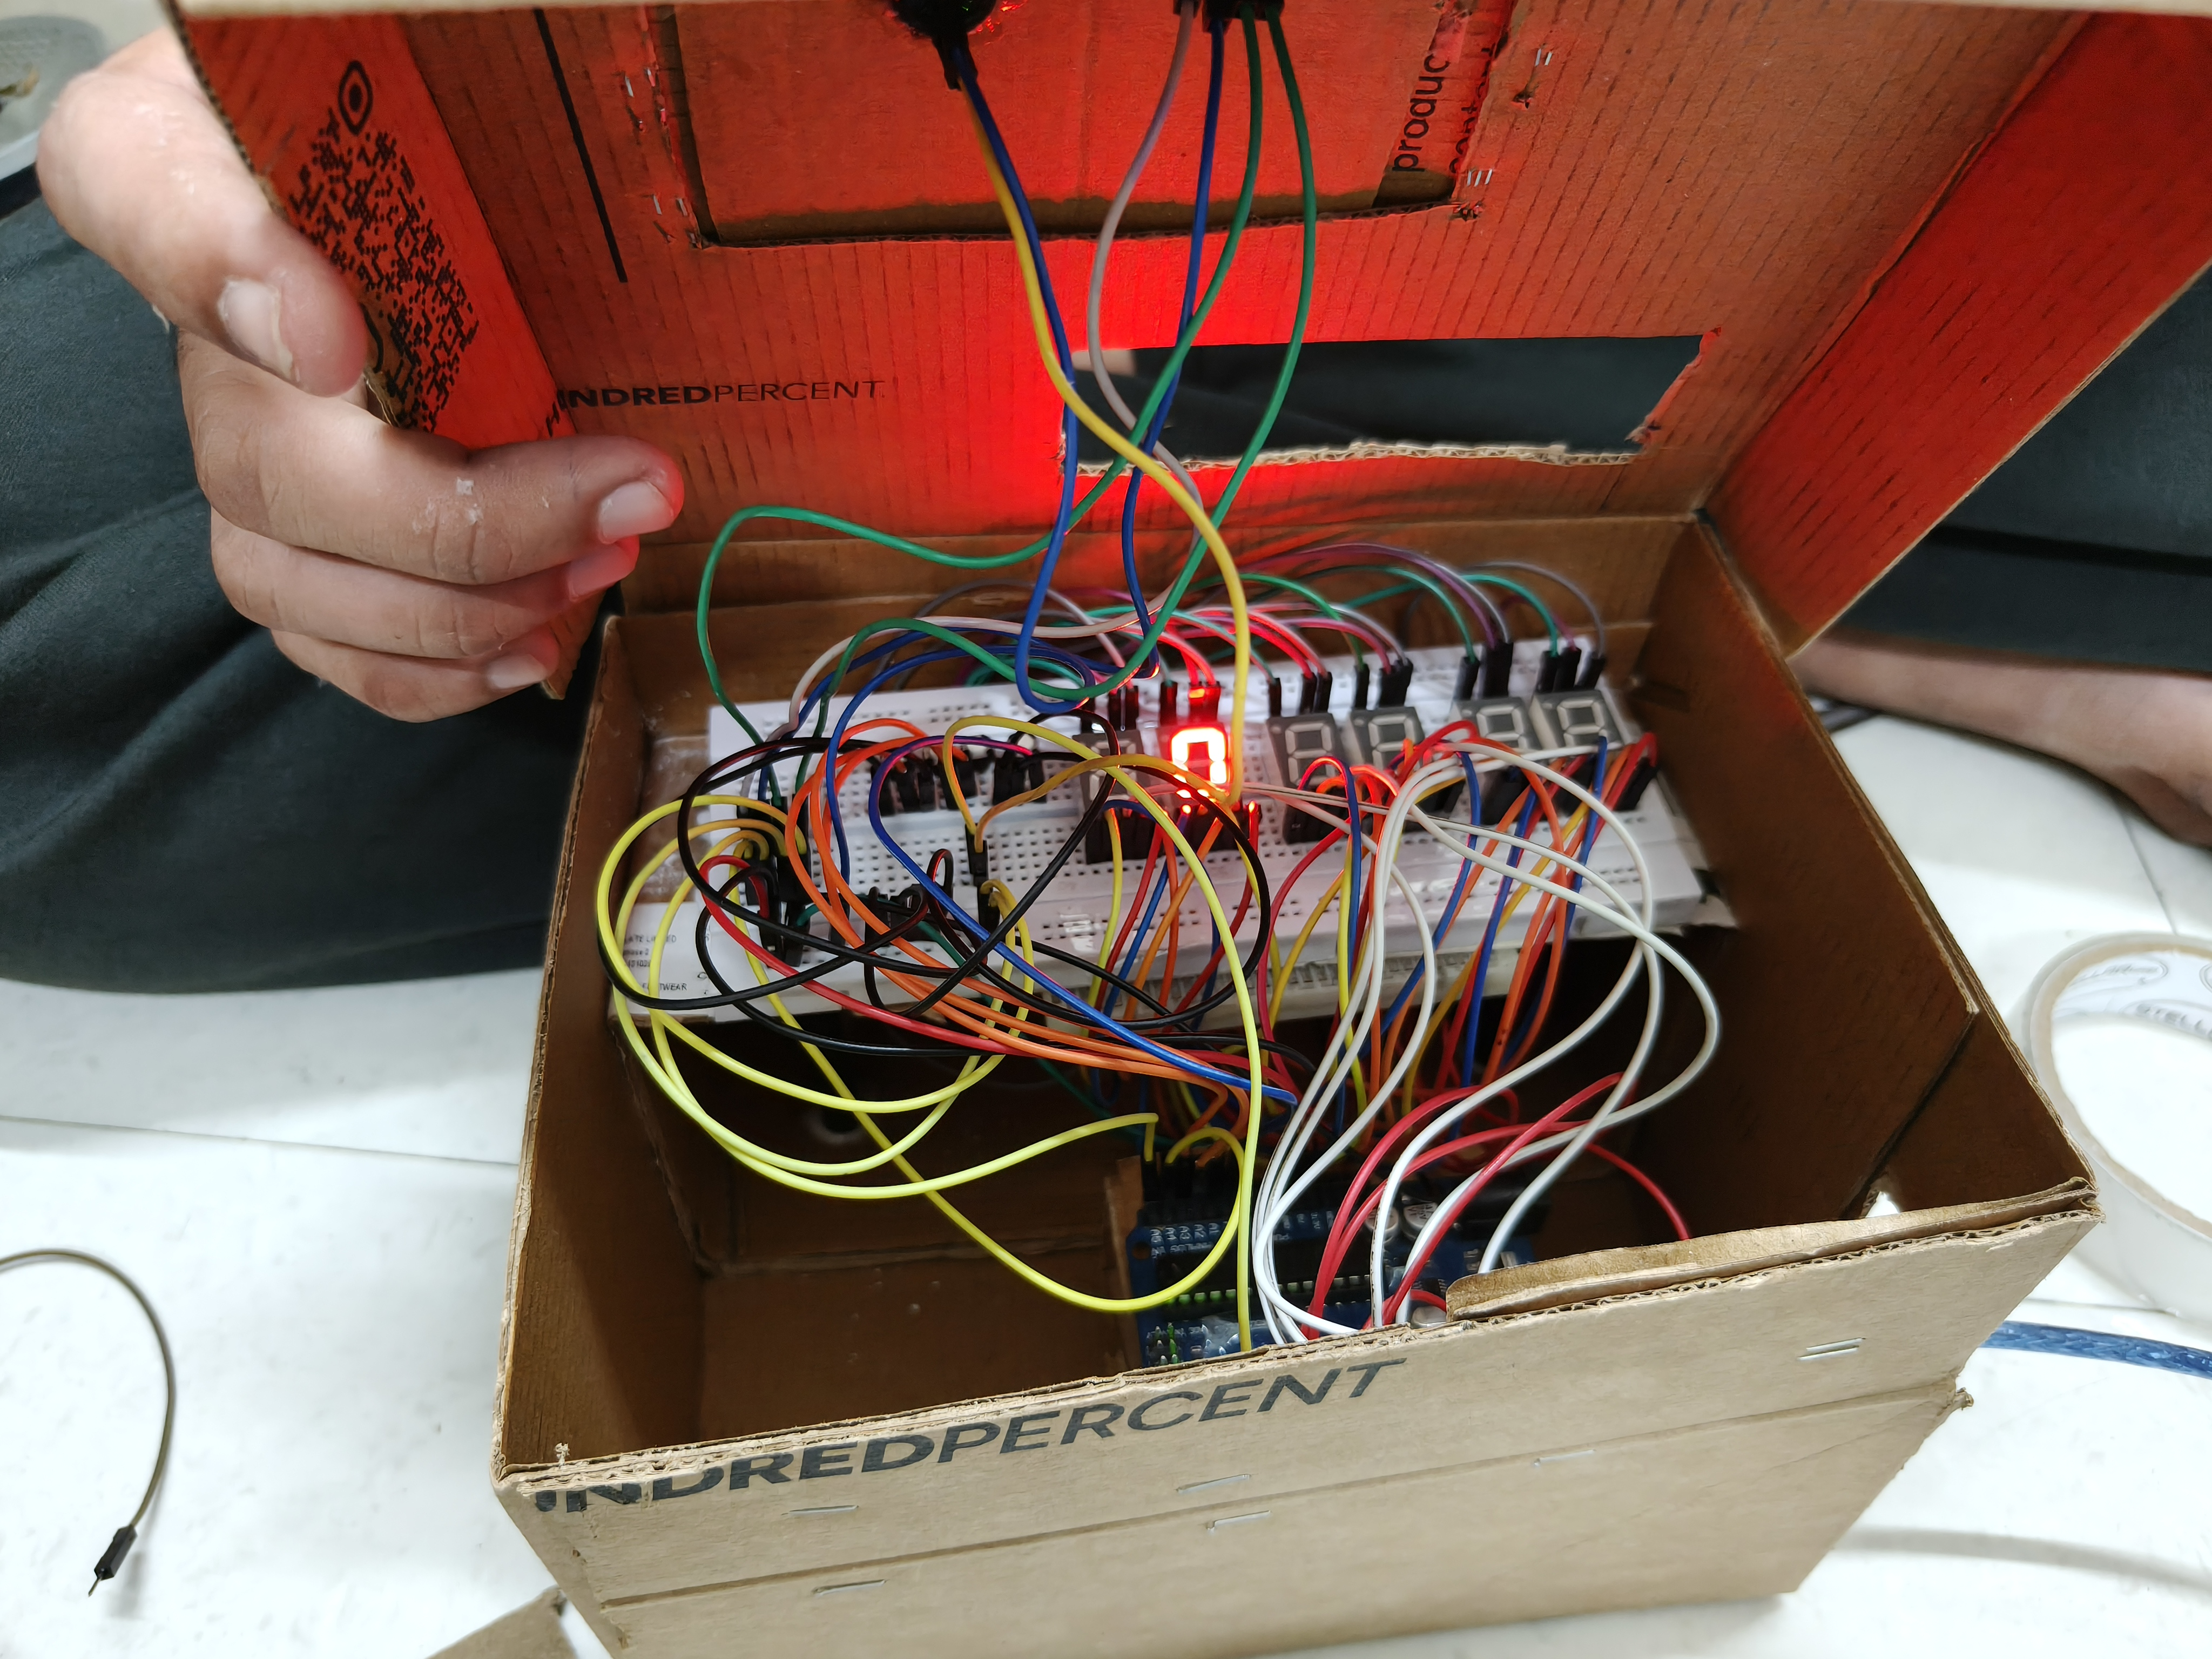
\includegraphics[width=0.88\textwidth,height=0.68\textheight,keepaspectratio]{images/9.jpg}
    \caption{No-touch OLED boxing.}
    \label{fig:visual-progress-9}
\end{figure}

\begin{figure}[H]
    \centering
    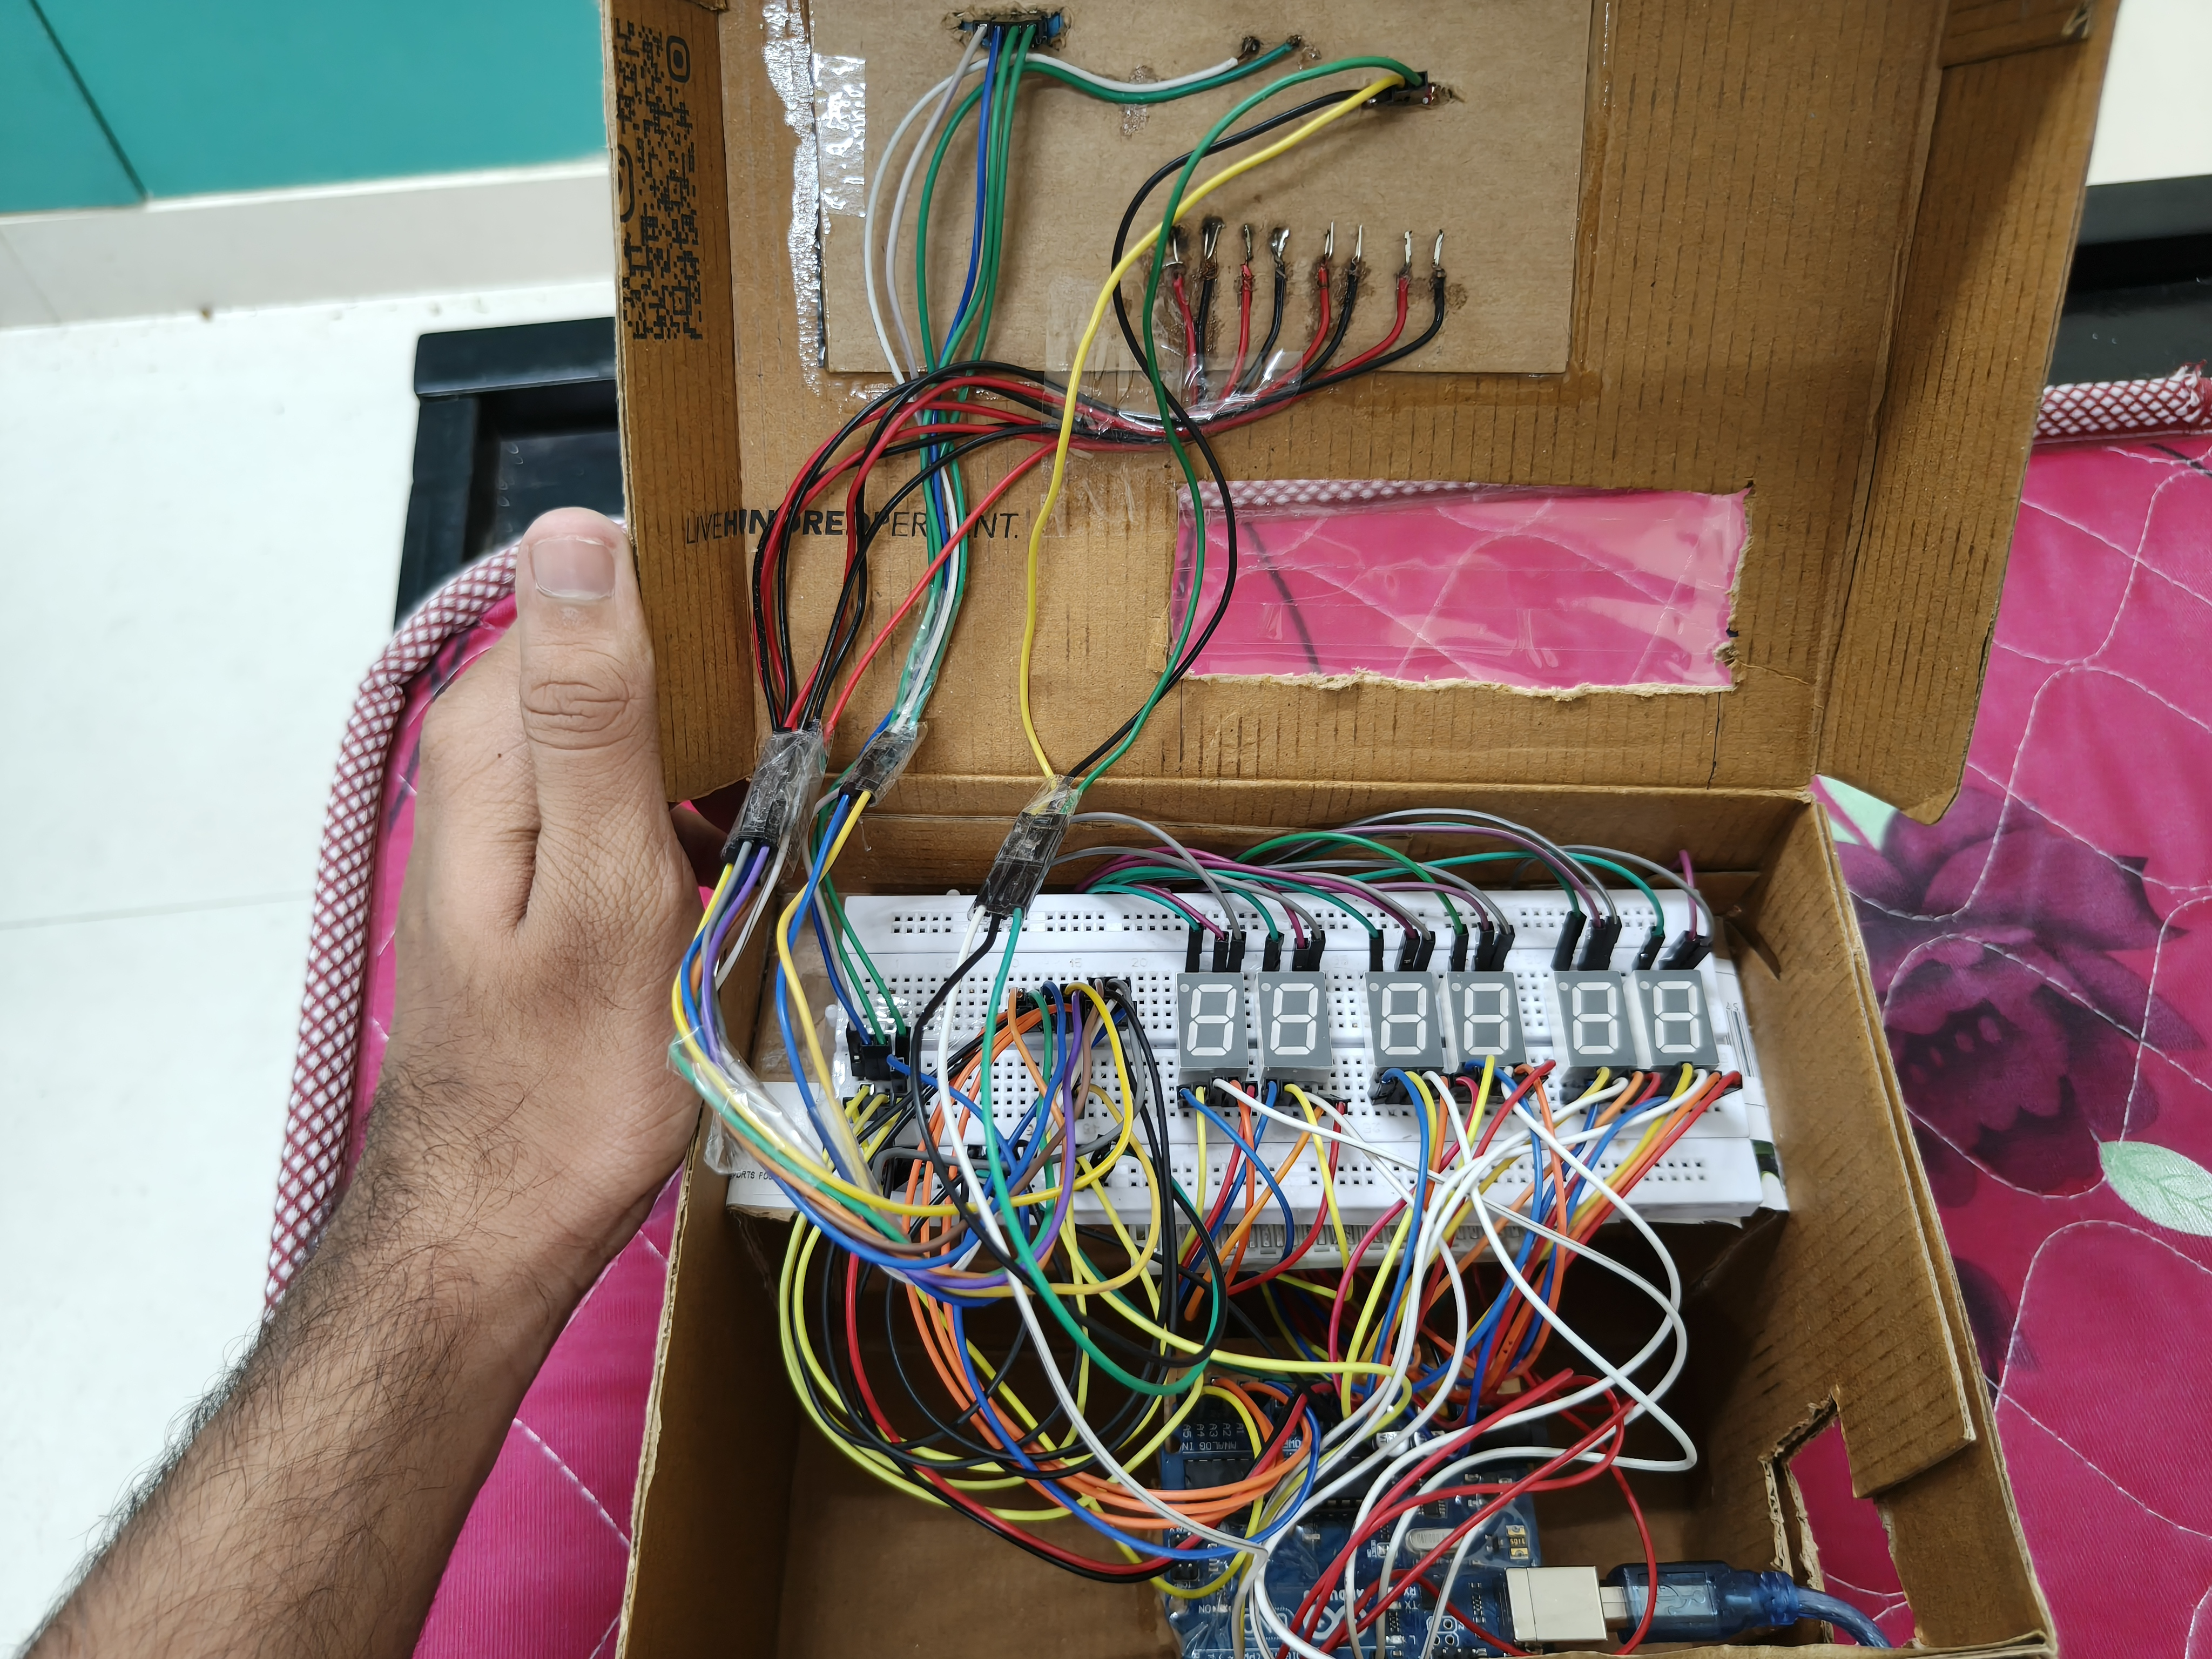
\includegraphics[width=0.88\textwidth,height=0.68\textheight,keepaspectratio]{images/10.jpg}
    \caption{Final wiring arrangement.}
    \label{fig:visual-progress-10}
\end{figure}

\begin{figure}[H]
    \centering
    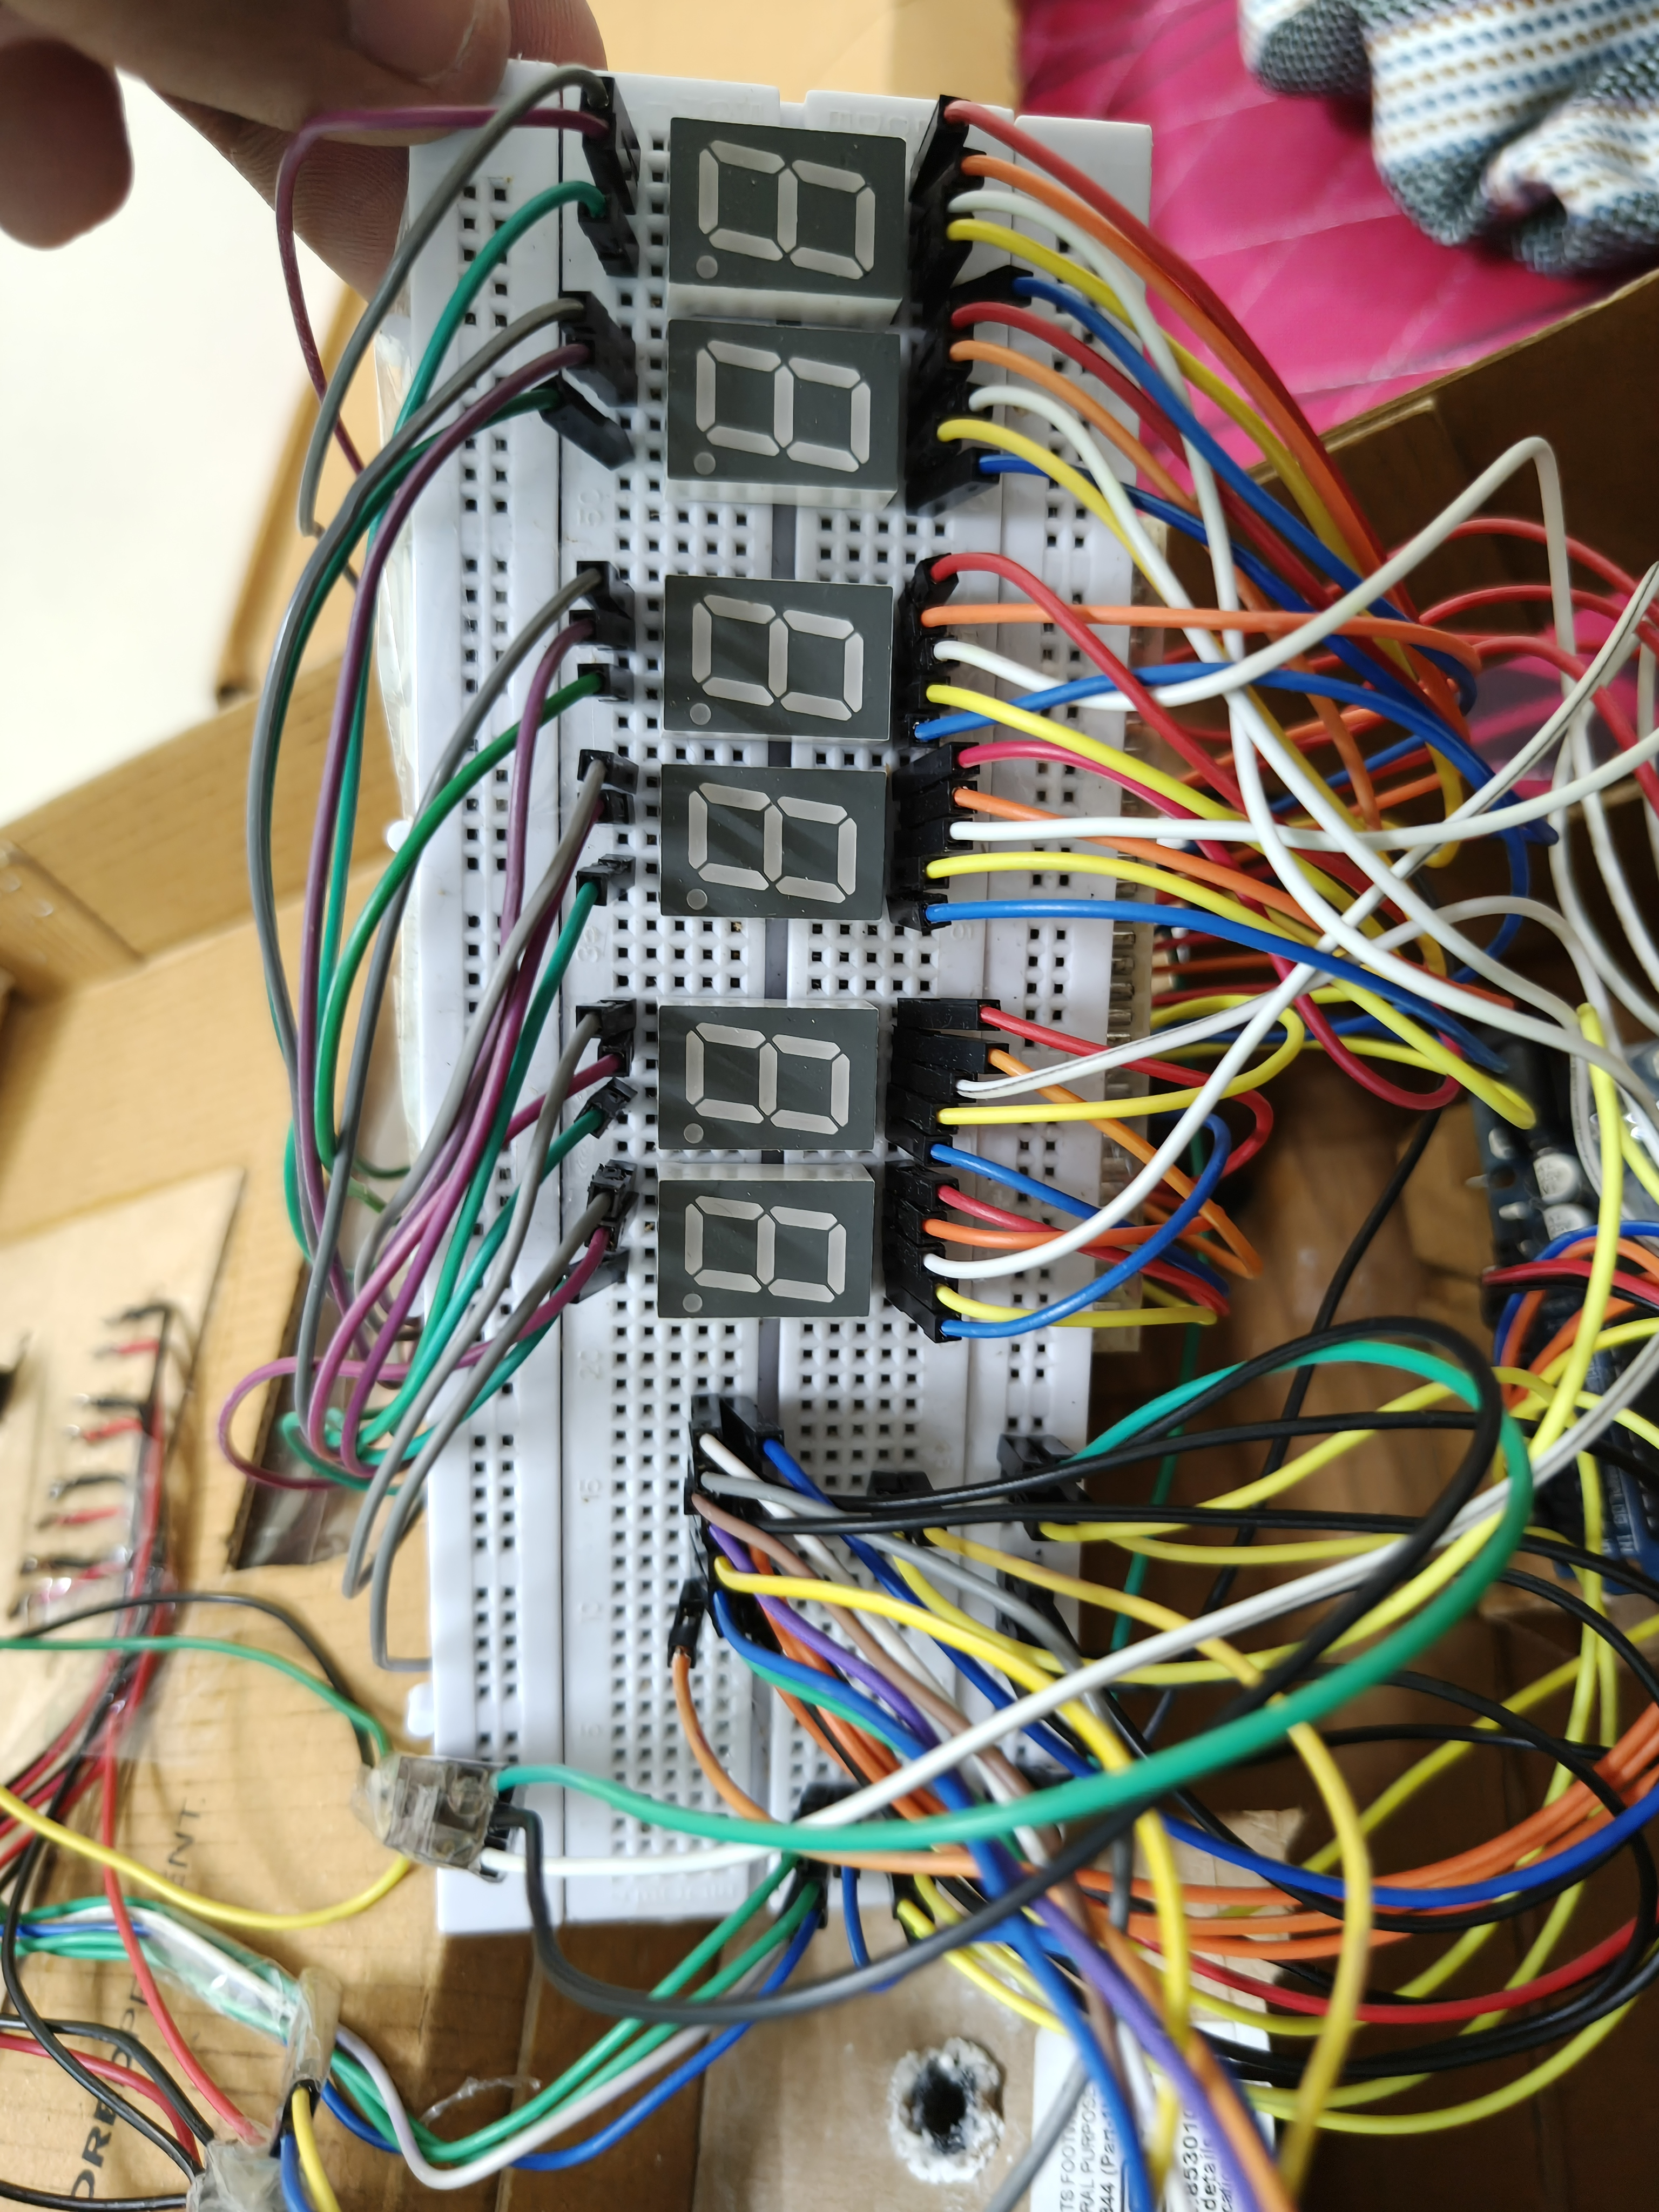
\includegraphics[width=0.88\textwidth,height=0.68\textheight,keepaspectratio]{images/11.jpg}
    \caption{Final front breadboard.}
    \label{fig:visual-progress-11}
\end{figure}

\begin{figure}[H]
    \centering
    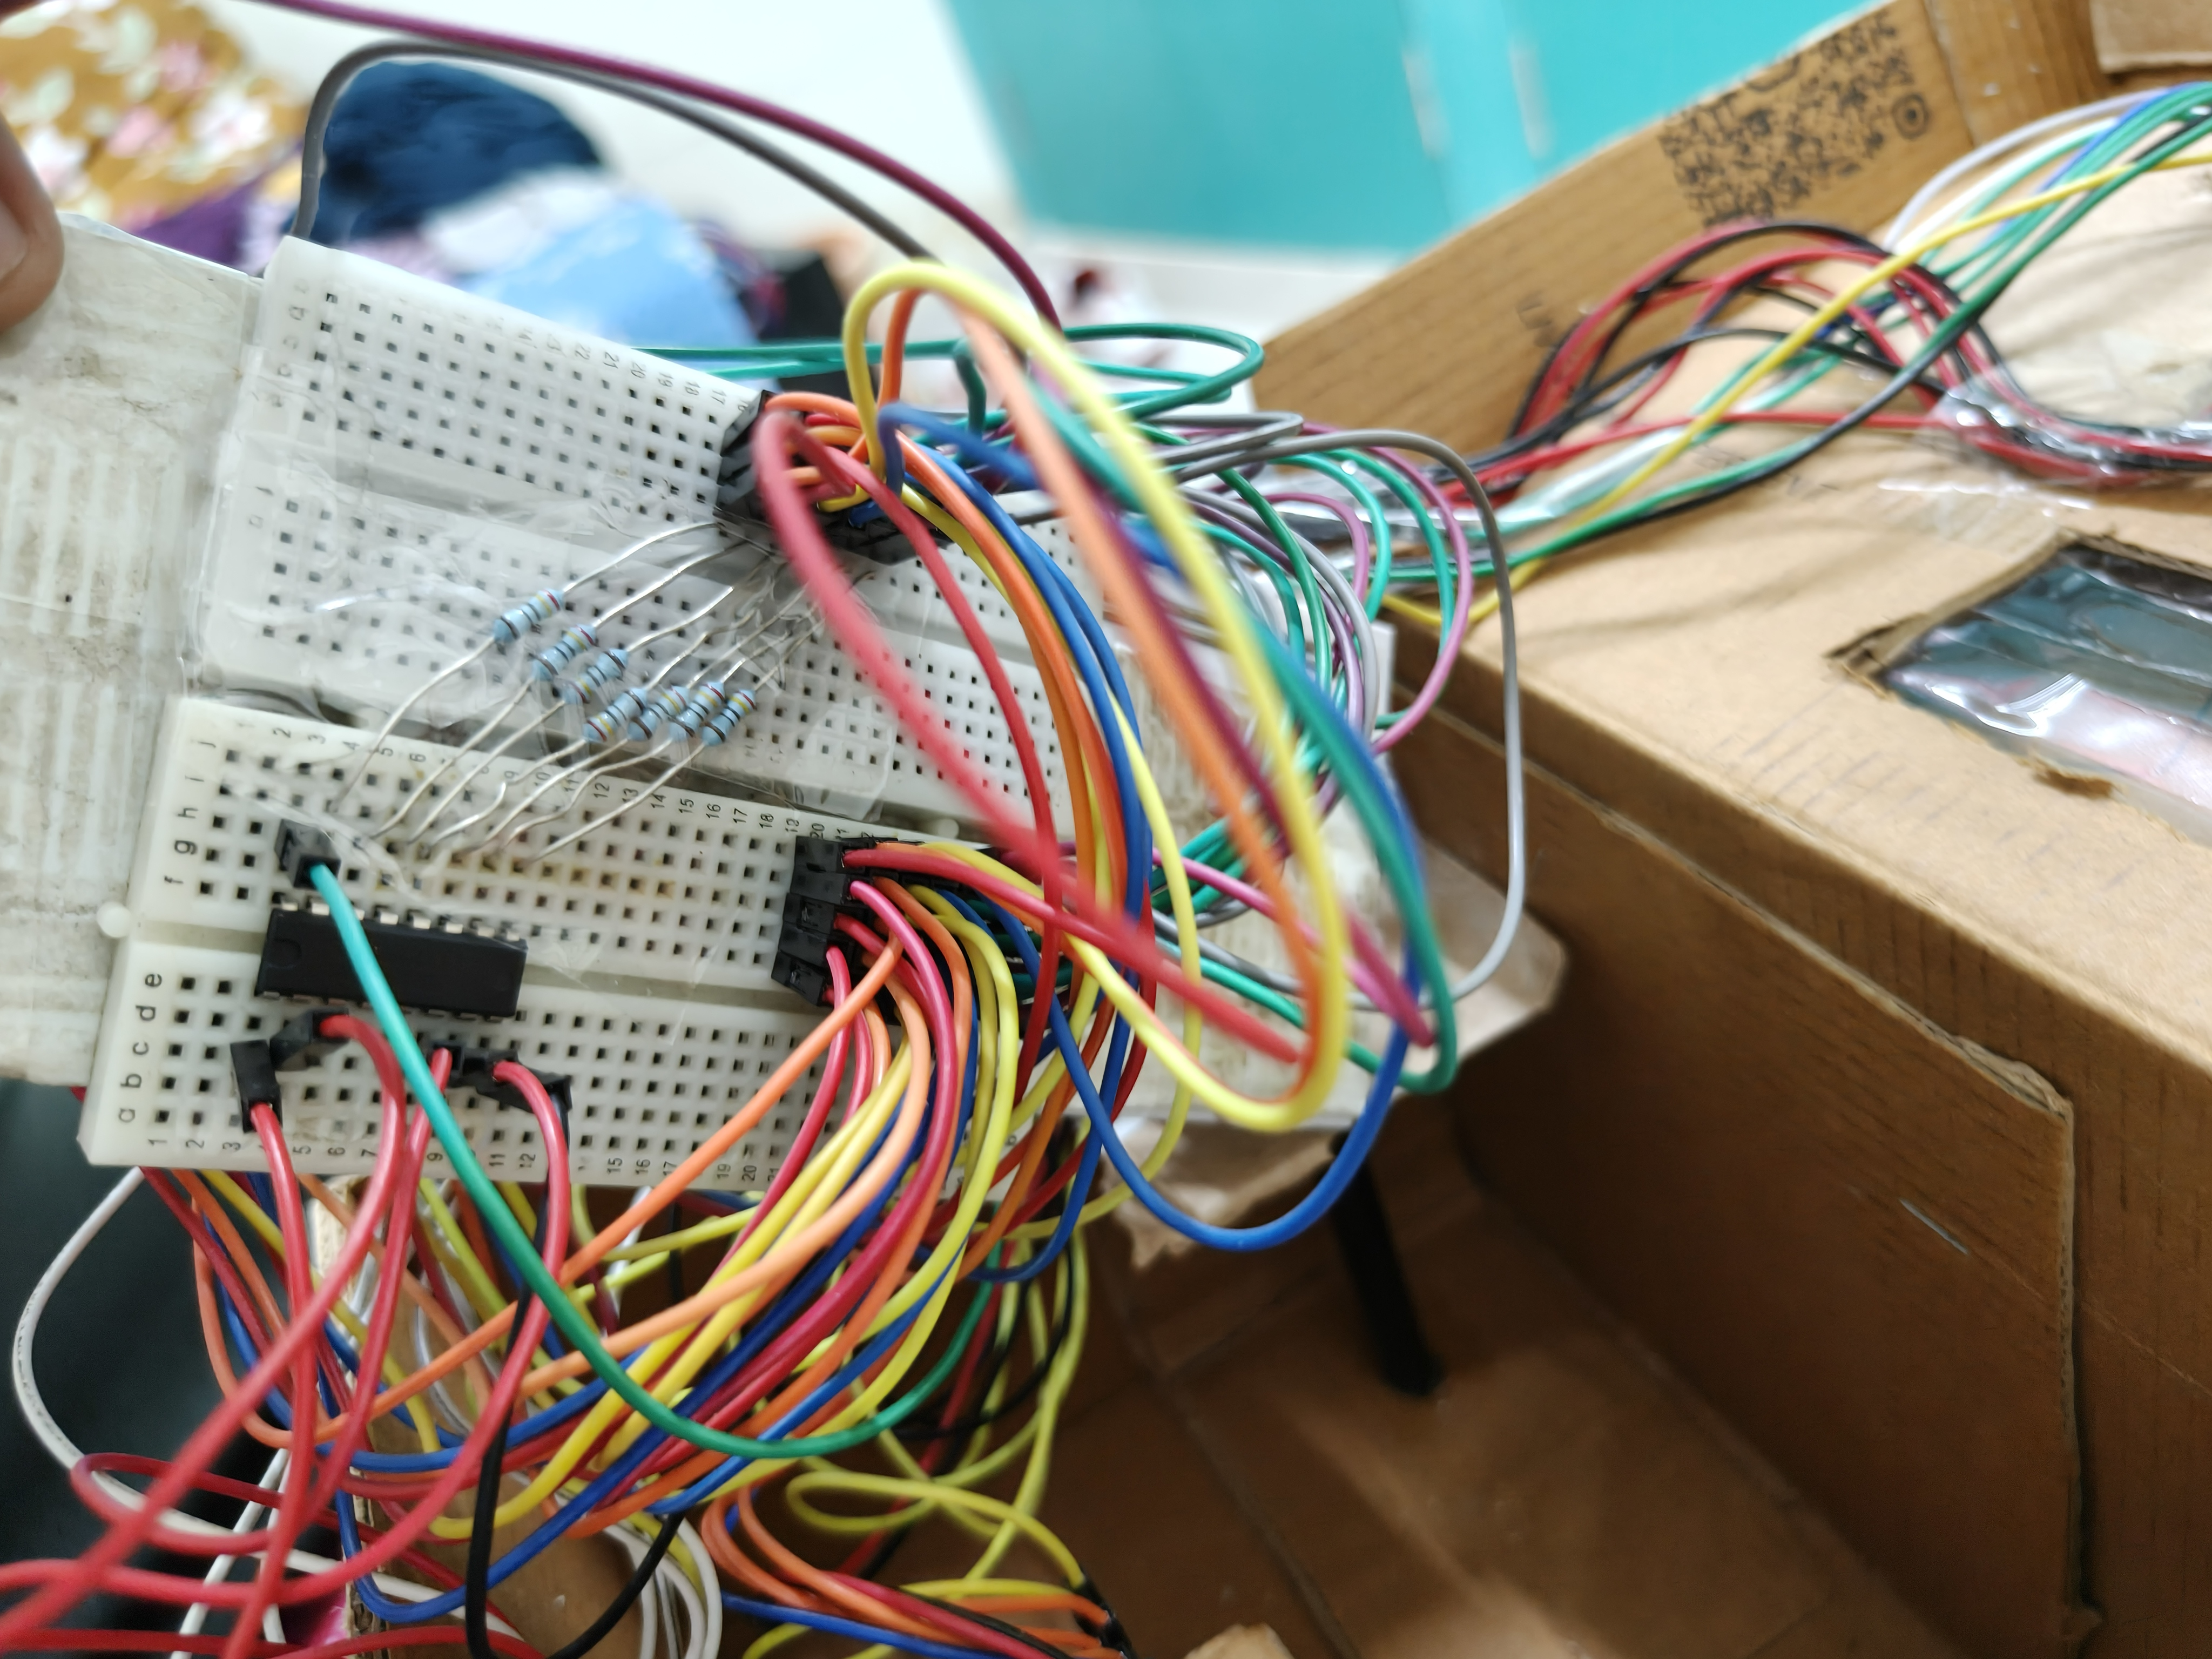
\includegraphics[width=0.88\textwidth,height=0.68\textheight,keepaspectratio]{images/12.jpg}
    \caption{Final second breadboard.}
    \label{fig:visual-progress-12}
\end{figure}

\begin{figure}[H]
    \centering
    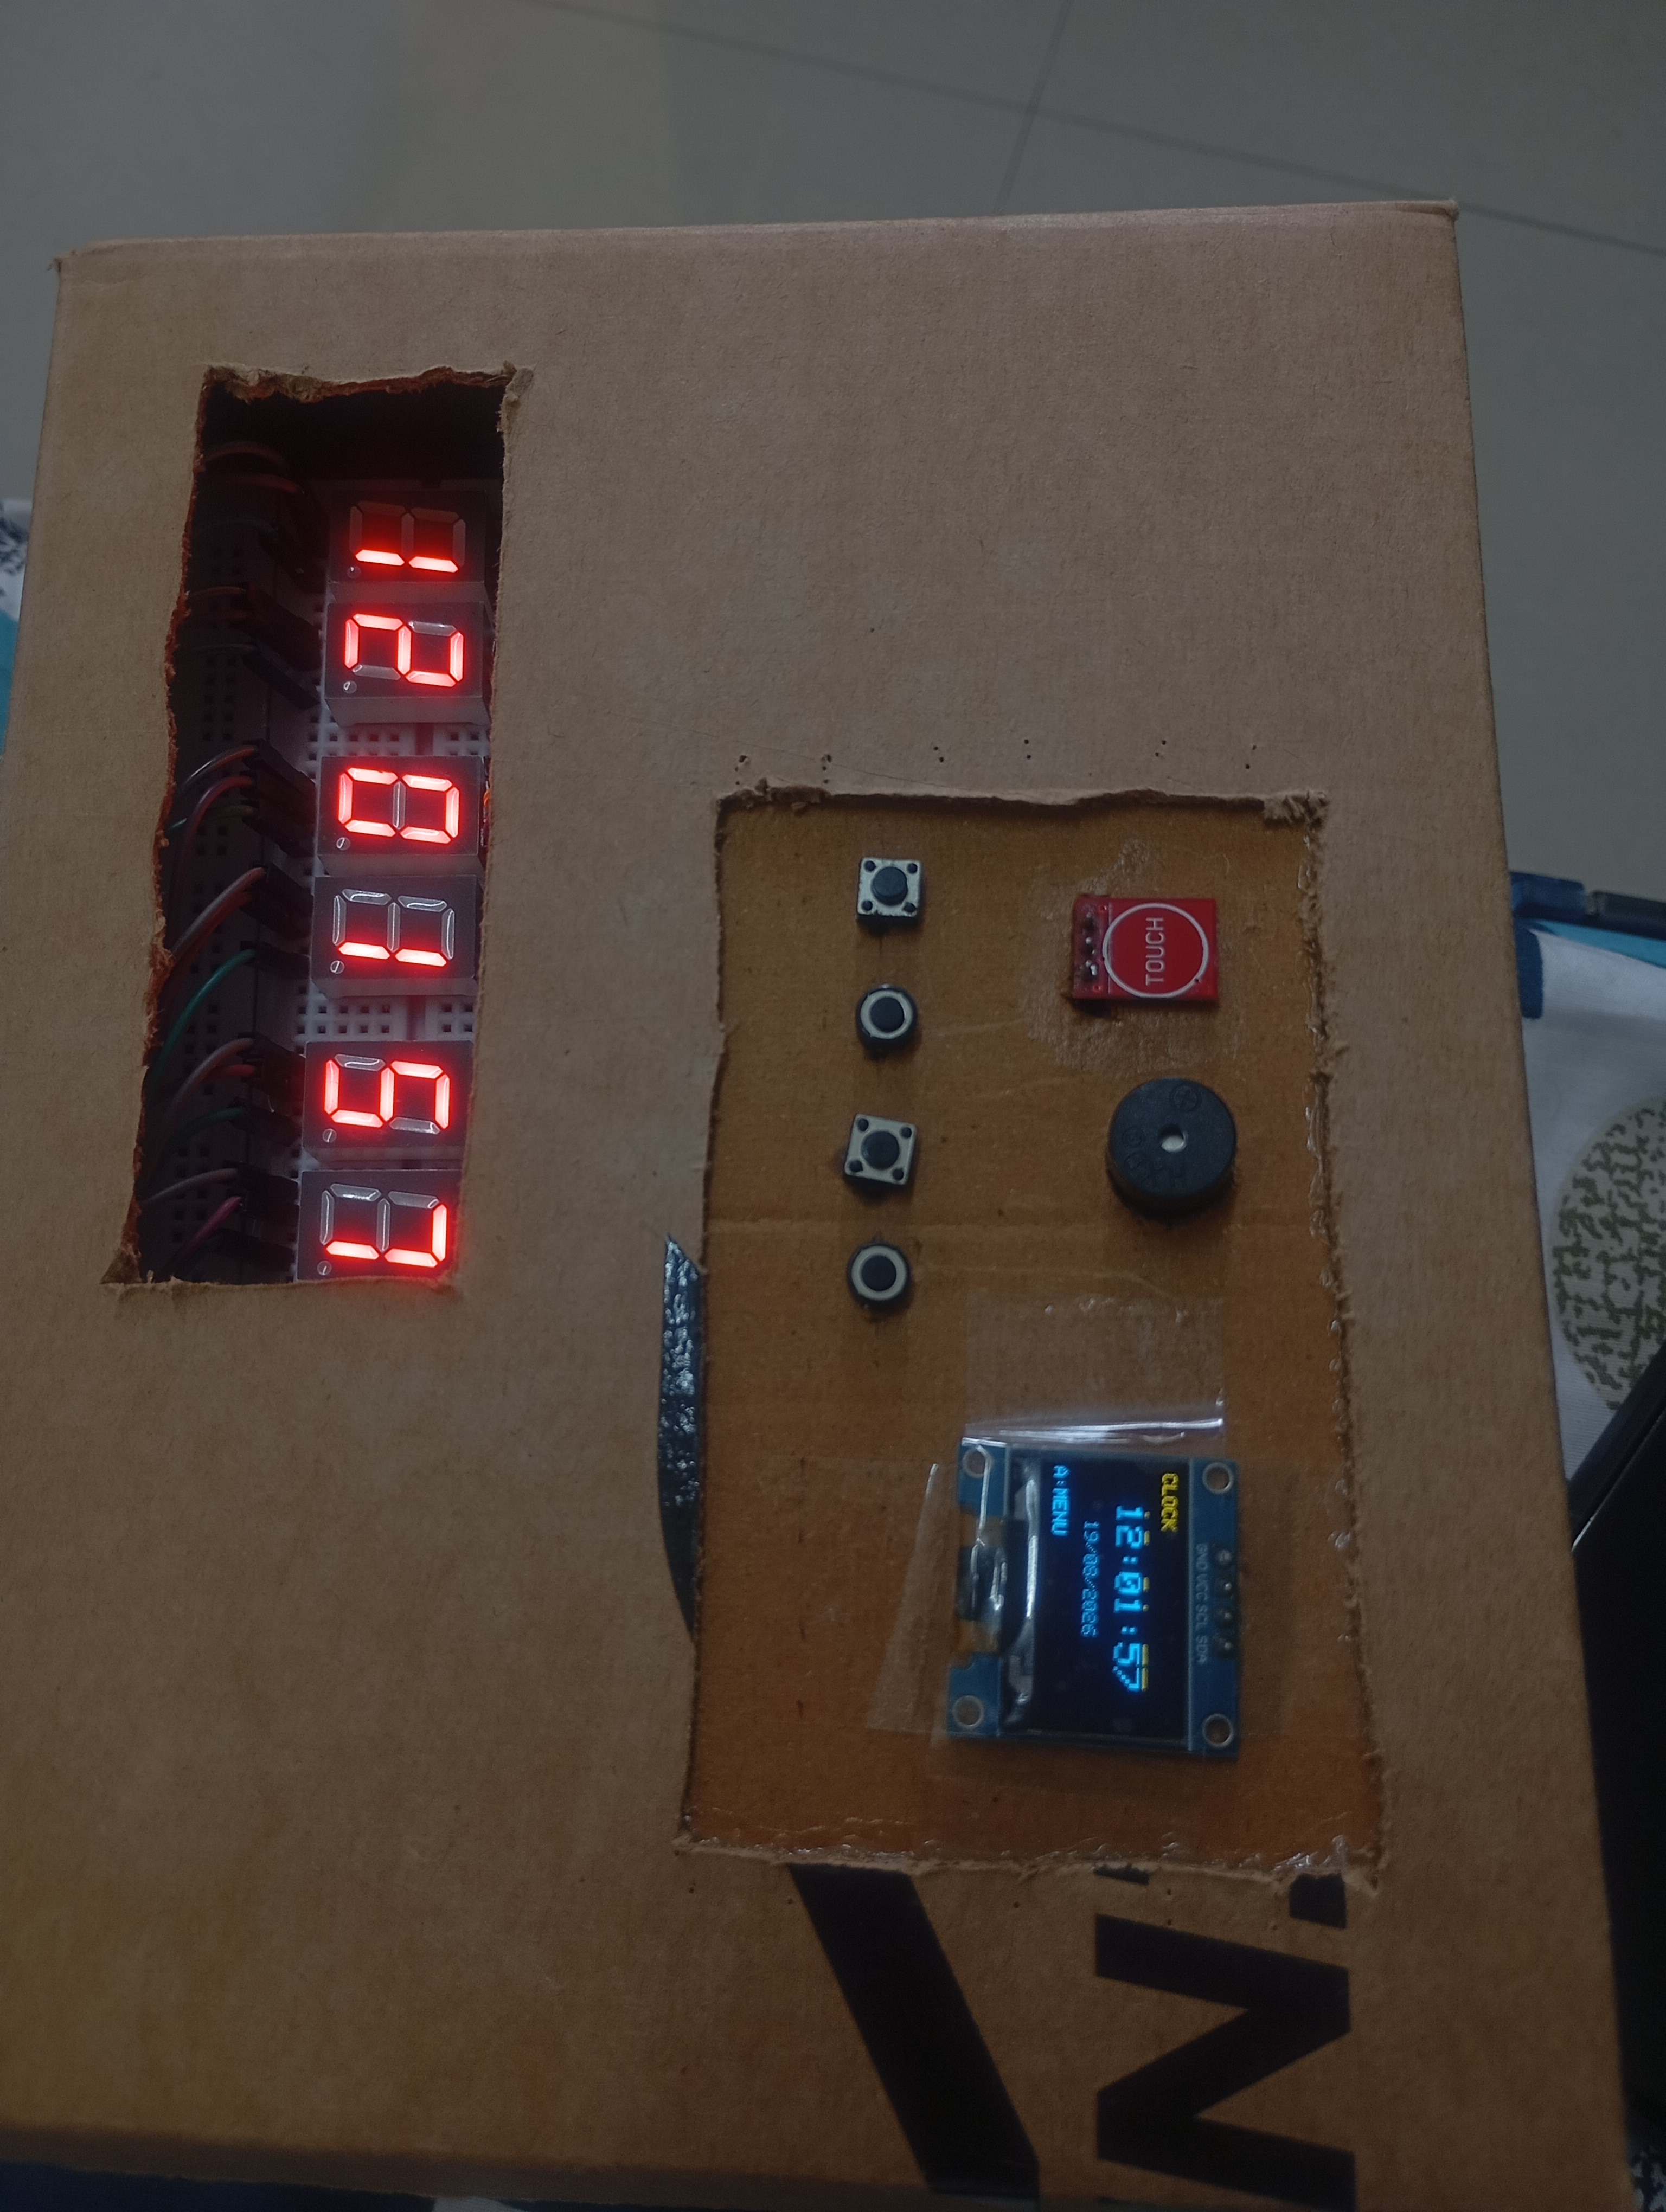
\includegraphics[width=0.88\textwidth,height=0.68\textheight,keepaspectratio]{images/13.jpg}
    \caption{Final working boxed prototype.}
    \label{fig:visual-progress-13}
\end{figure}

\subsection{Basic Engineering Applications}


\begin{figure}[H]
    \centering
    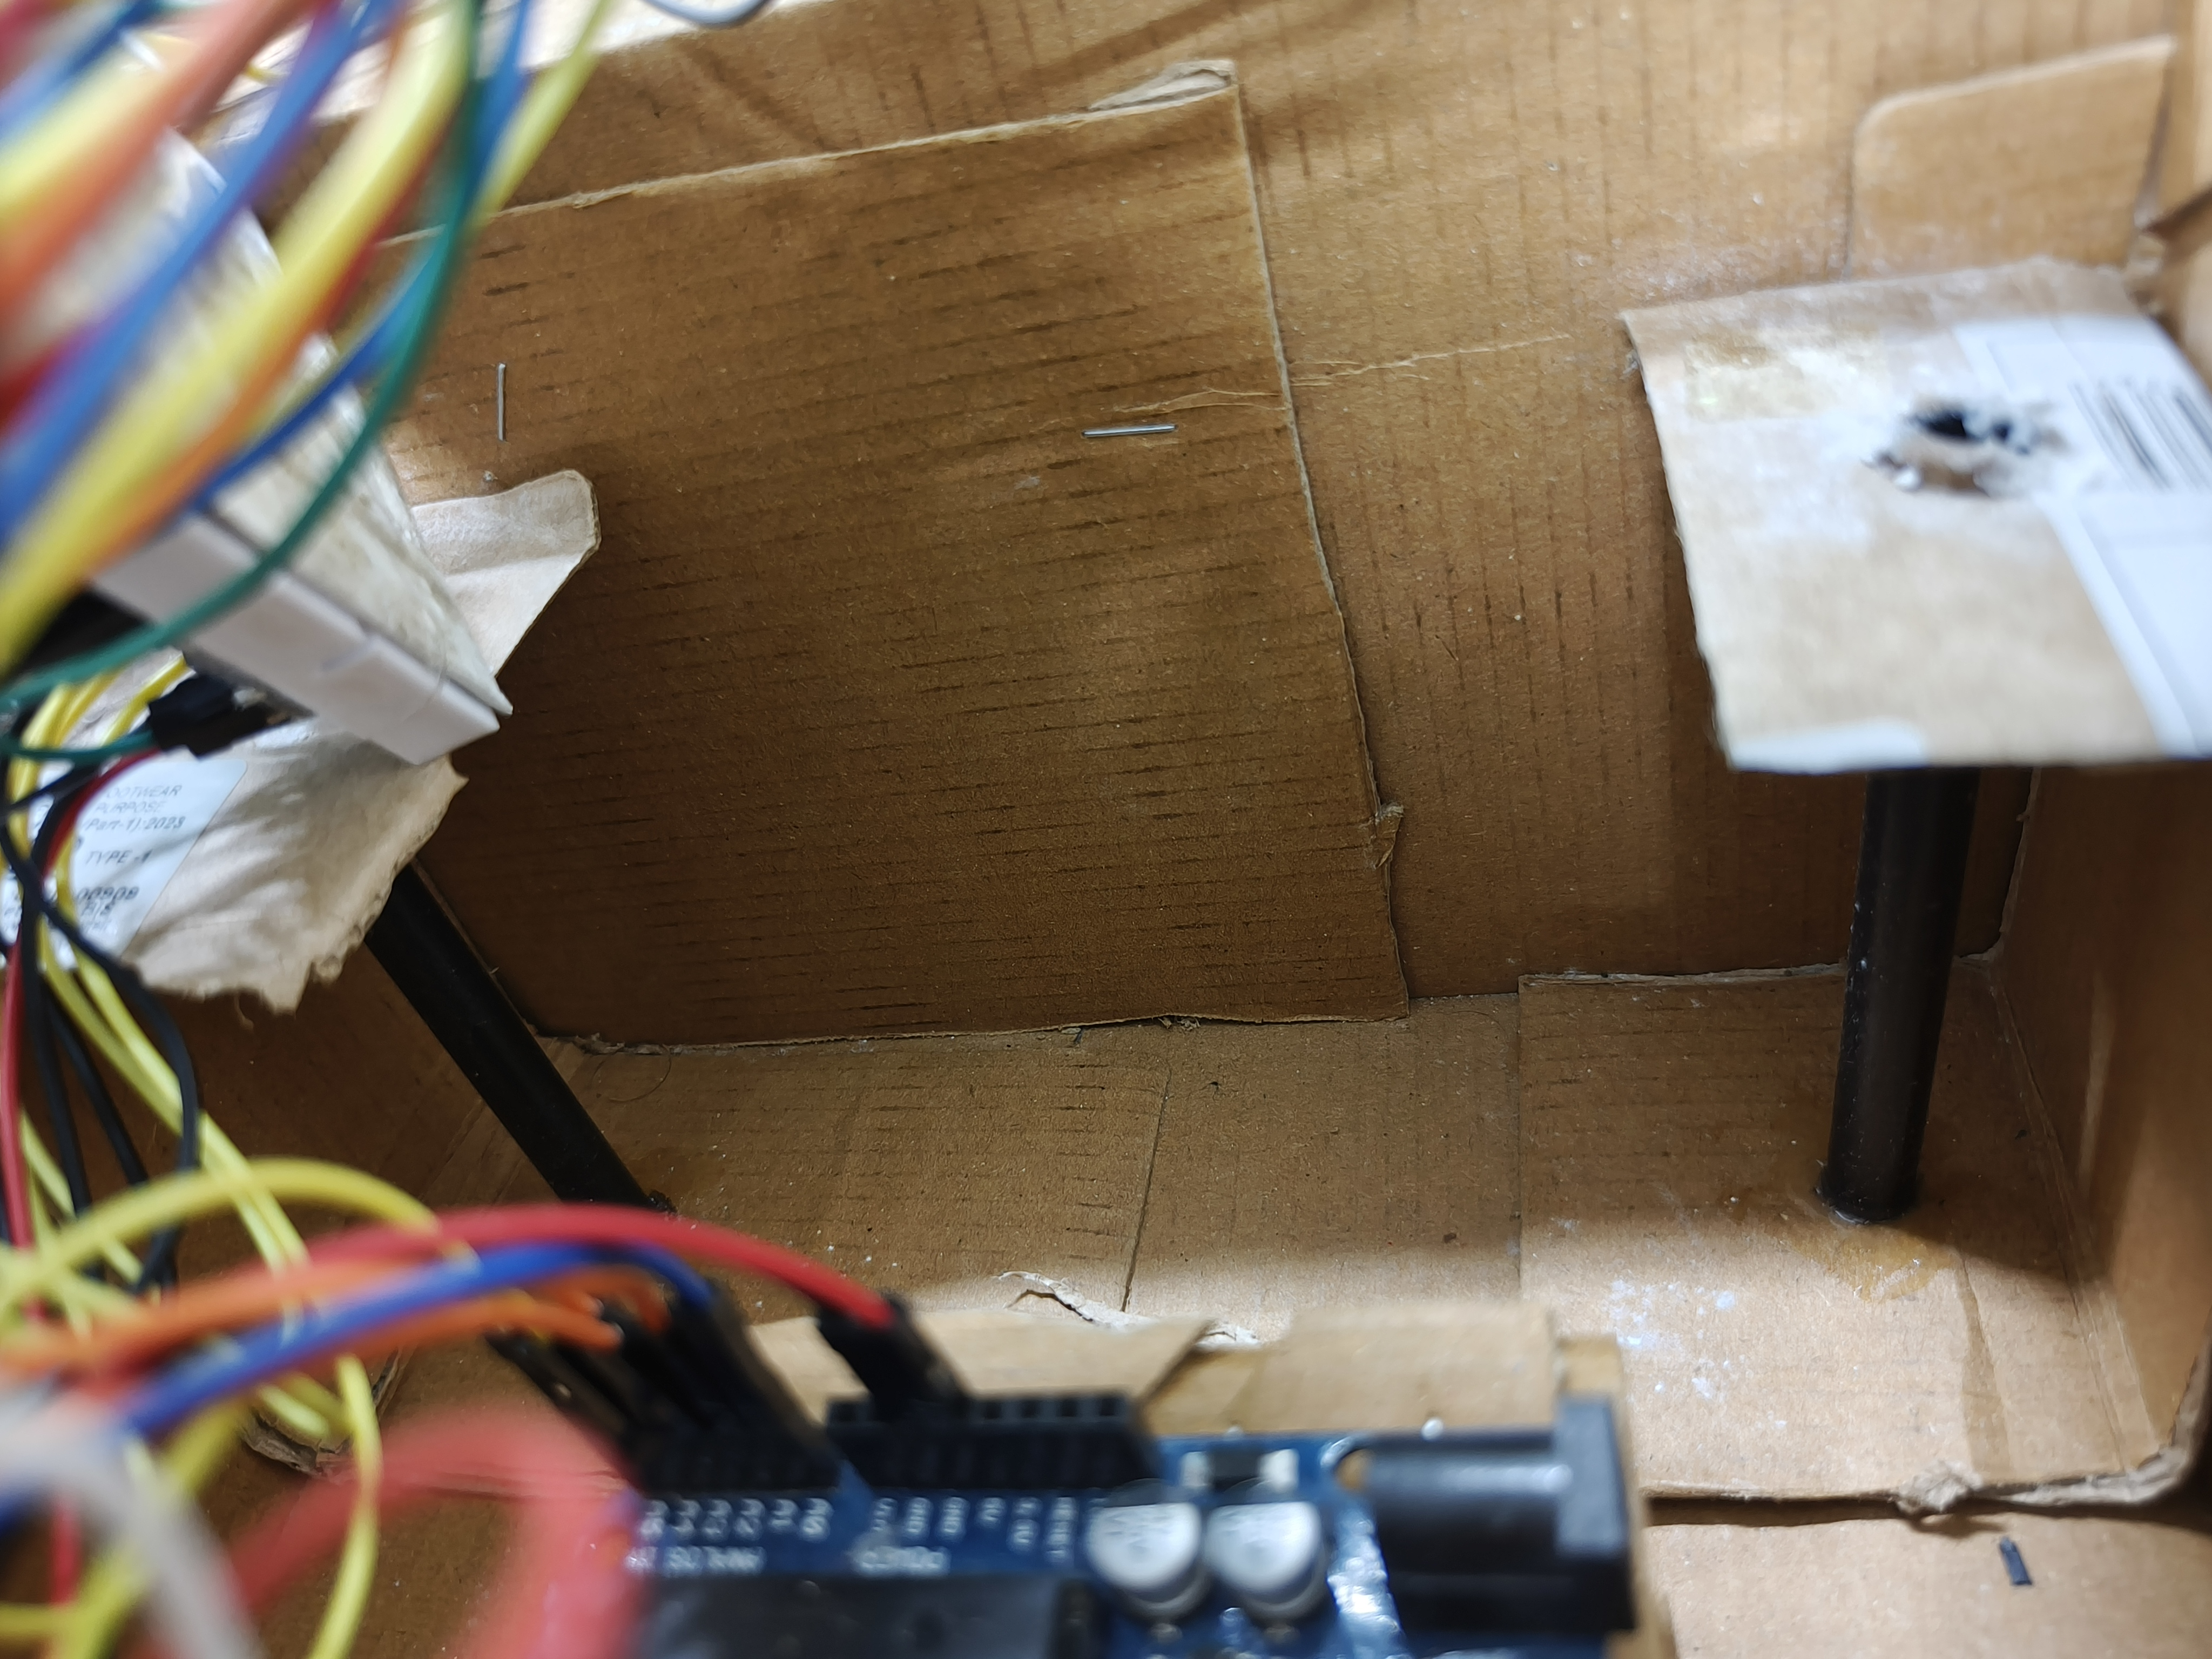
\includegraphics[width=0.88\textwidth,height=0.68\textheight,keepaspectratio]{images/14.jpg}
    \caption{Final breadboard support.}
    \label{fig:visual-progress-14}
\end{figure}

\begin{figure}[H]
    \centering
    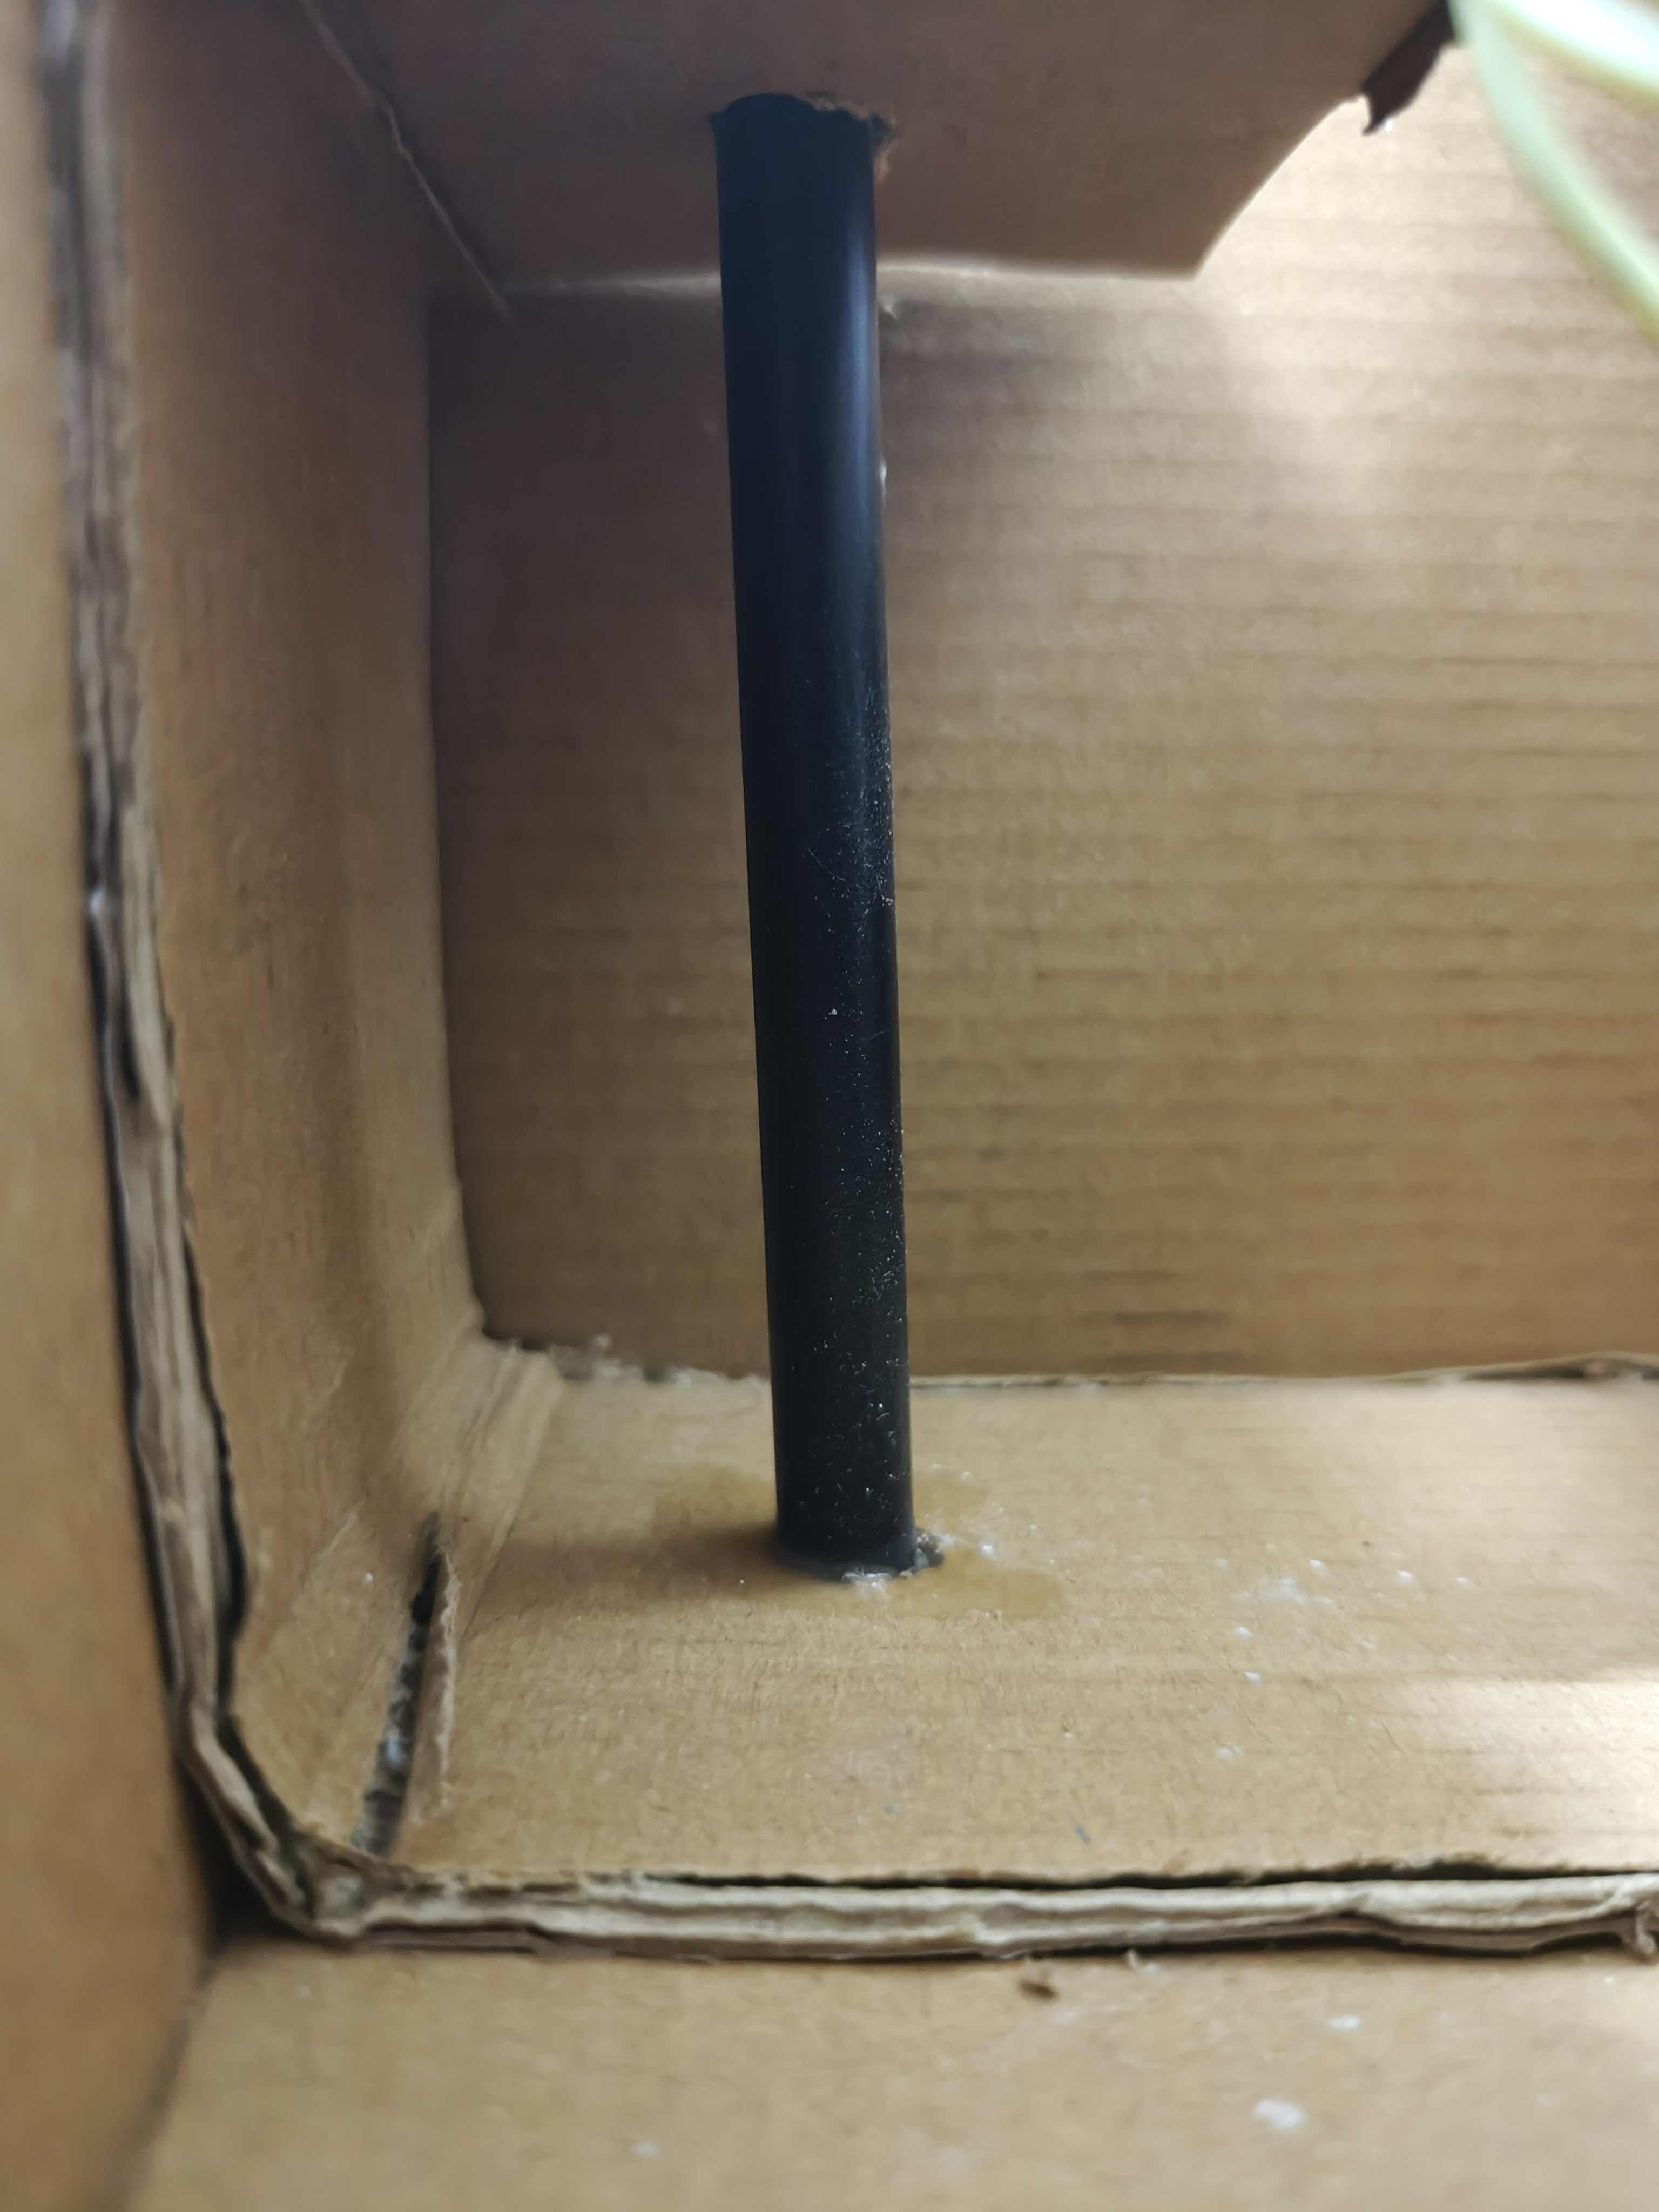
\includegraphics[width=0.88\textwidth,height=0.68\textheight,keepaspectratio]{images/15.jpg}
    \caption{Support pillars.}
    \label{fig:visual-progress-15}
\end{figure}

\begin{figure}[H]
    \centering
    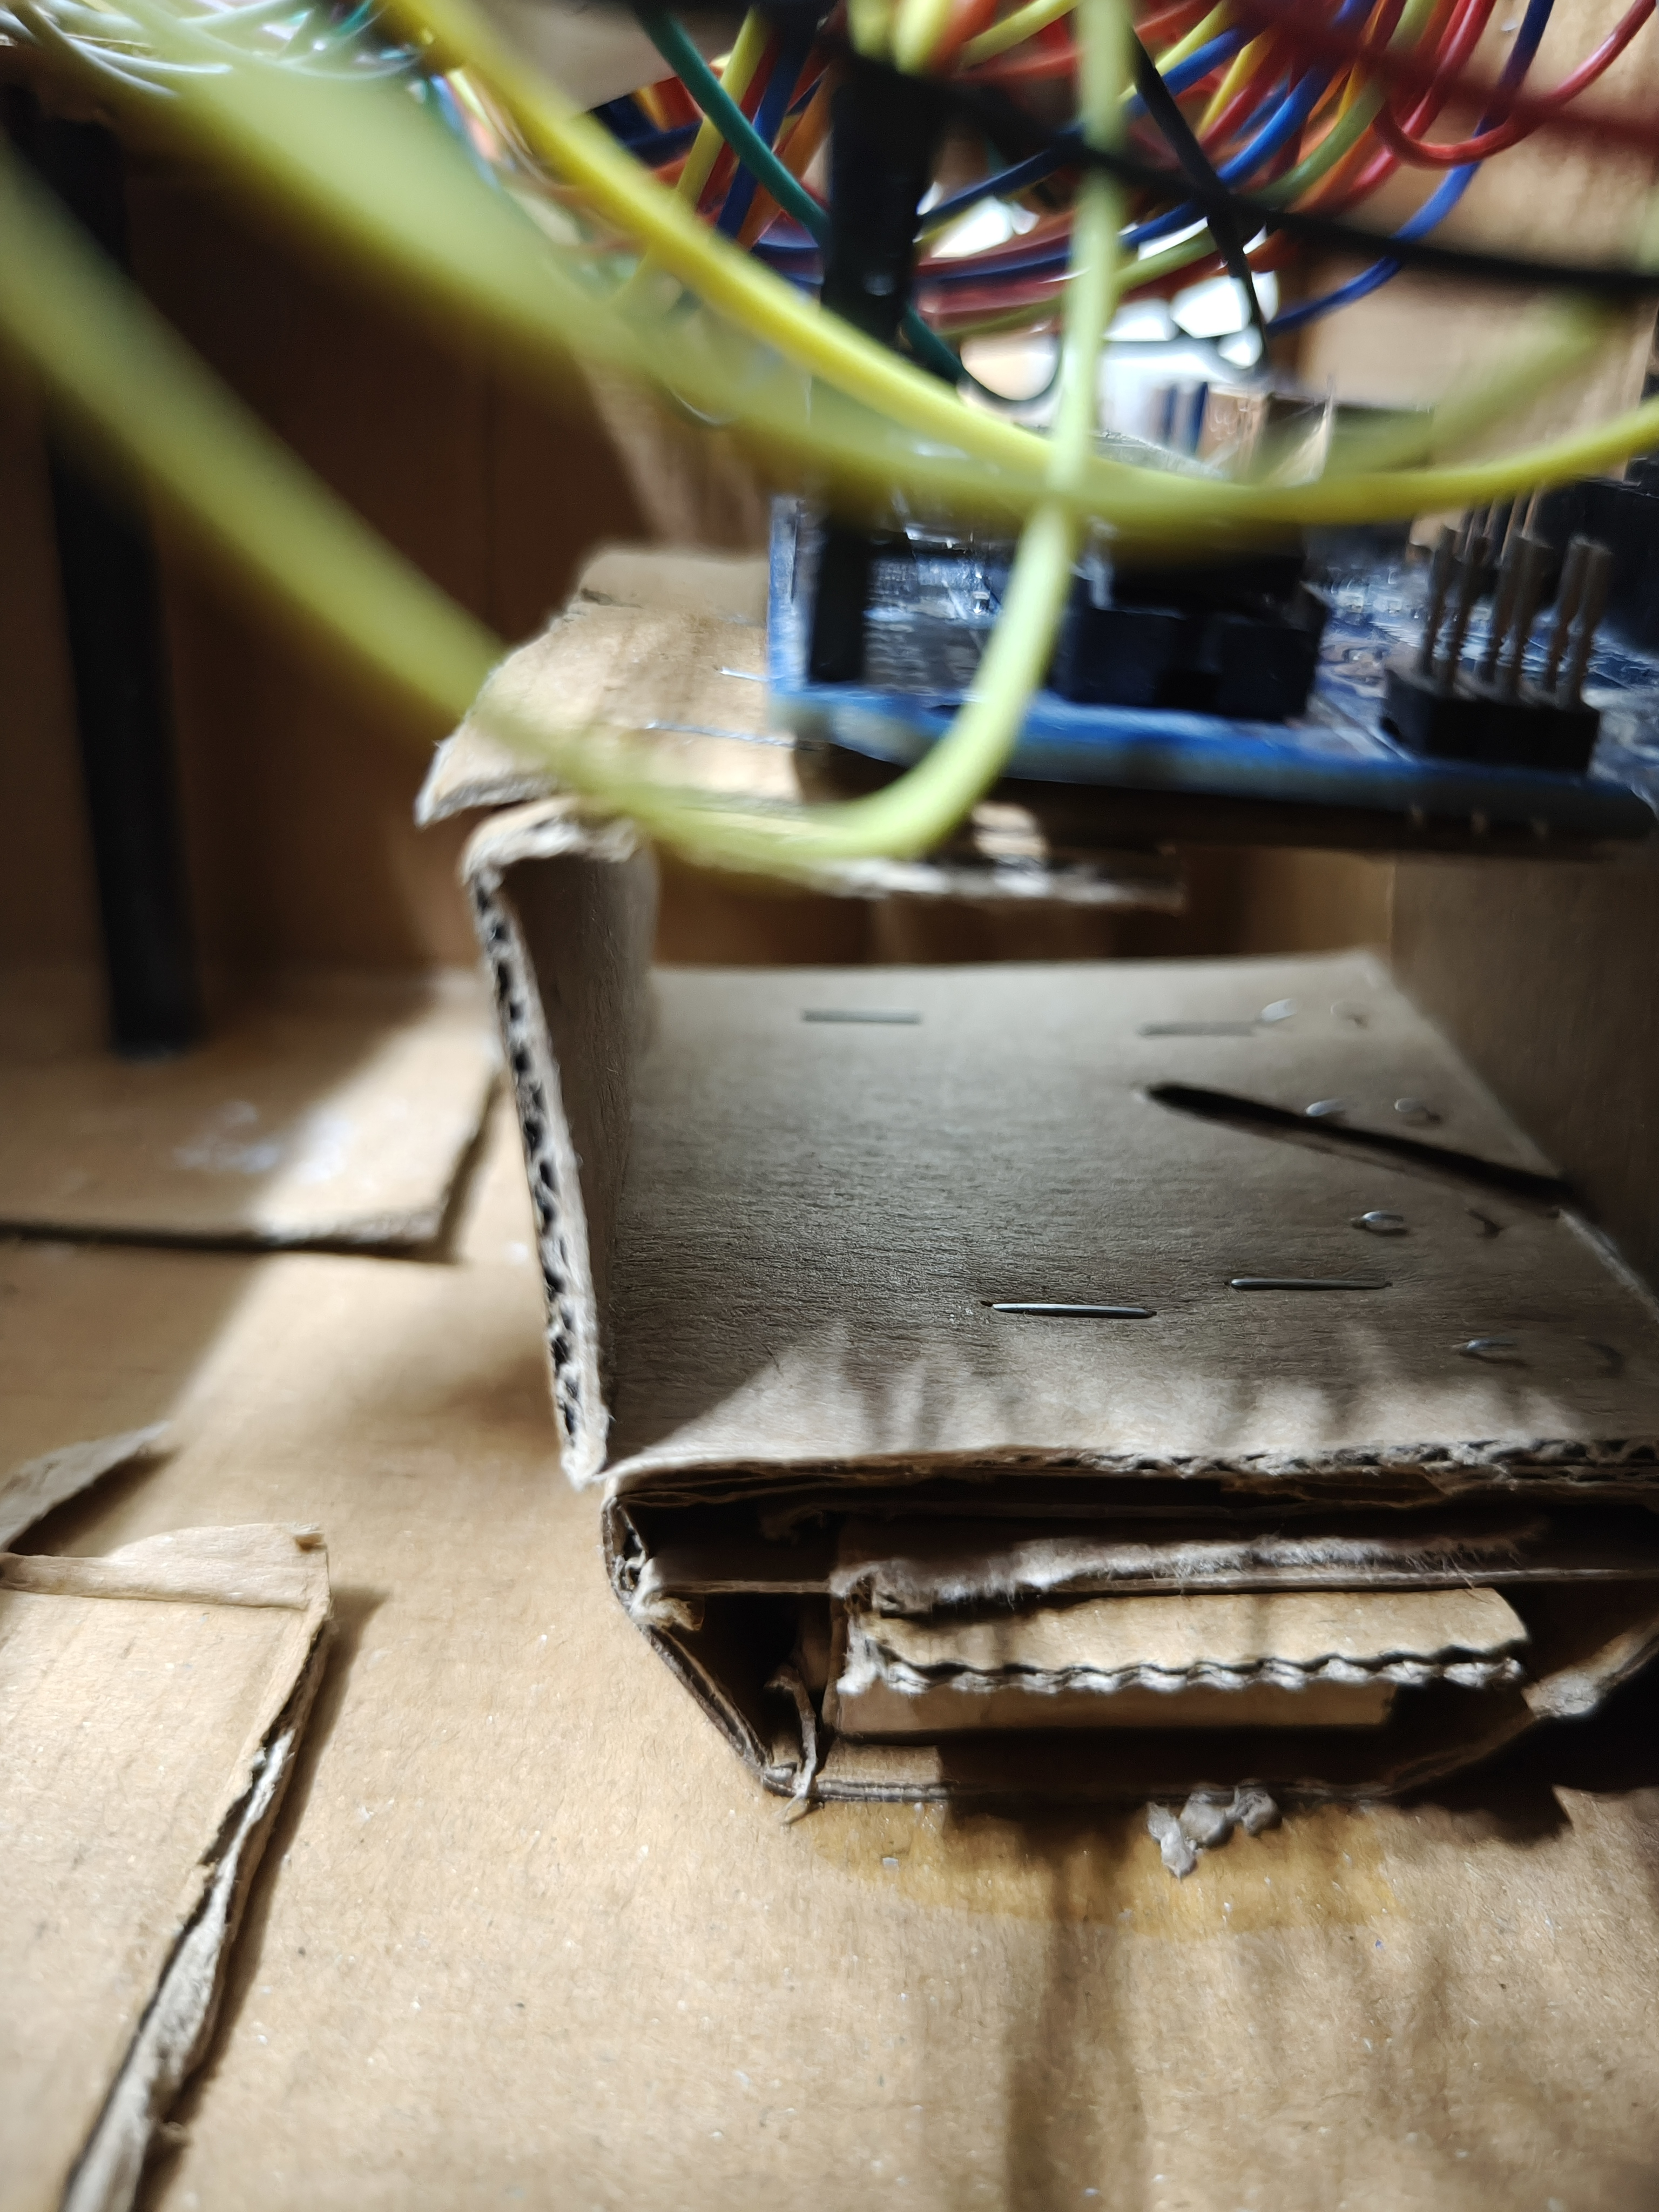
\includegraphics[width=0.88\textwidth,height=0.68\textheight,keepaspectratio]{images/16.jpg}
    \caption{Arduino holding stand.}
    \label{fig:visual-progress-16}
\end{figure}

\section{Video Development Journey}

A supplementary video record of the project development and demonstrations is
available in the following playlist:

\begin{center}
\url{https://www.youtube.com/playlist?list=PLJr6fgl30GfY}
\end{center}

\end{document}